\documentclass{article}
\RequirePackage[utf8]{inputenc}
\RequirePackage[T1]{fontenc}
\RequirePackage{amsmath}
\RequirePackage{bytefield}
\RequirePackage{graphicx}
\RequirePackage{newtxmath}
\RequirePackage{mathtools}
\RequirePackage{xspace}
\RequirePackage{url}
\RequirePackage{changepage}
\RequirePackage{enumitem}
\RequirePackage{tabularx}
\RequirePackage{hhline}
\RequirePackage[usestackEOL]{stackengine}
\RequirePackage{comment}
\RequirePackage{needspace}
\RequirePackage[nobottomtitles]{titlesec}
\RequirePackage[hang]{footmisc}
\RequirePackage{xstring}
\RequirePackage[unicode,bookmarksnumbered,bookmarksopen]{hyperref}
\RequirePackage{cleveref}
\RequirePackage{nameref}
\RequirePackage{etoolbox}
\RequirePackage{subdepth}

\RequirePackage[style=alphabetic,maxbibnames=99,dateabbrev=false,urldate=iso8601,backref=true,backrefstyle=none,backend=biber]{biblatex}
\addbibresource{zcash.bib}

% Fonts
\RequirePackage{lmodern}
\RequirePackage{quattrocento}
\RequirePackage[bb=ams]{mathalfa}

% Quattrocento is beautiful but doesn't have an italic face. So we scale
% New Century Schoolbook italic to fit in with slanted Quattrocento and
% match its x height.
\renewcommand{\emph}[1]{\hspace{0.15em}{\fontfamily{pnc}\selectfont\scalebox{1.02}[0.999]{\textit{#1}}}\hspace{0.02em}}

% While we're at it, let's match the tt x height to Quattrocento as well.
\let\oldtexttt\texttt
\let\oldmathtt\mathtt
\renewcommand{\texttt}[1]{\scalebox{1.02}[1.07]{\oldtexttt{#1}}}
\renewcommand{\mathtt}[1]{\scalebox{1.02}[1.07]{$\oldmathtt{#1}$}}

% bold but not extended
\newcommand{\textbnx}[1]{{\fontseries{b}\selectfont #1}}


\crefformat{footnote}{#2\footnotemark[#1]#3}

\DeclareLabelalphaTemplate{
  \labelelement{\field{citekey}}
}

\DefineBibliographyStrings{english}{
  page  = {page},
  pages = {pages},
  backrefpage = {\mbox{$\uparrow$ p\!}},
  backrefpages = {\mbox{$\uparrow$ p\!}}
}

\setlength{\oddsidemargin}{-0.25in}
\setlength{\textwidth}{7in}
\setlength{\topmargin}{-0.75in}
\setlength{\textheight}{9.2in}
\setlength{\parindent}{0ex}
\renewcommand{\arraystretch}{1.4}
\overfullrule=2cm

\setlength{\footnotemargin}{0.6em}
\setlength{\footnotesep}{2ex}
\addtolength{\skip\footins}{3ex}

\renewcommand{\bottomtitlespace}{8ex}

% Use rubber lengths between paragraphs to improve default pagination.
% https://tex.stackexchange.com/questions/17178/vertical-spacing-pagination-and-ideal-results
\setlength{\parskip}{1.5ex plus 1pt minus 1pt}

\setlist[enumerate]{before=\vspace{-1ex}}
\setlist[itemize]{itemsep=0.5ex,topsep=0.2ex,before=\vspace{-1ex},after=\vspace{1.5ex}}

\newlist{formulae}{itemize}{3}
\setlist[formulae]{itemsep=0.2ex,topsep=0ex,leftmargin=1.5em,label=,after=\vspace{1.5ex}}

\newlist{lines}{itemize}{3}
\setlist[lines]{itemsep=-0.5ex,topsep=0ex,before=\vspace{1ex},leftmargin=1.5em,label=,after=\vspace{1ex}}

\newcommand{\docversion}{Version unavailable (check protocol.ver)}
\newtoggle{issapling}
\togglefalse{issapling}
\InputIfFileExists{protocol.ver}{}{}

\newcommand{\doctitle}{Zcash Protocol Specification}
\newcommand{\leadauthor}{Daira Hopwood}
\newcommand{\coauthora}{Sean Bowe}
\newcommand{\coauthorb}{Taylor Hornby}
\newcommand{\coauthorc}{Nathan Wilcox}

\newcommand{\keywords}{anonymity, applications, cryptographic protocols,\
electronic commerce and payment, financial privacy, proof of work, zero knowledge}

\hypersetup{
  pdfborderstyle={/S/U/W 0.7},
  pdfinfo={
    Title={\doctitle, \docversion},
    Author={\leadauthor, \coauthora, \coauthorb, \coauthorc},
    Keywords={\keywords}
  }
}

\makeatletter
\renewcommand*{\@fnsymbol}[1]{\ensuremath{\ifcase#1\or \dagger\or \ddagger\or
    \mathsection\or \mathparagraph\else\@ctrerr\fi}}
\makeatother

\renewcommand{\sectionautorefname}{\S\!}
\renewcommand{\subsectionautorefname}{\S\!}
\renewcommand{\subsubsectionautorefname}{\S\!}
\renewcommand{\paragraphautorefname}{\S\!}
\renewcommand{\subparagraphautorefname}{\S\!}
\newcommand{\crossref}[1]{\autoref{#1}\, \emph{`\nameref*{#1}\kern -0.05em'} on p.\,\pageref*{#1}}

% https://tex.stackexchange.com/a/60212/78411
\newcommand{\subsubsubsection}[1]{\paragraph{#1}\mbox{}\\}
\setcounter{secnumdepth}{4}
\setcounter{tocdepth}{4}

\newcommand{\nstrut}[1]{\texorpdfstring{#1\rule[-.2\baselineskip]{0pt}{\baselineskip}}{#1}}
\newcommand{\nsection}[1]{\section{\nstrut{#1}}}
\newcommand{\nsubsection}[1]{\subsection{\nstrut{#1}}}
\newcommand{\nsubsubsection}[1]{\subsubsection{\nstrut{#1}}}
\newcommand{\nsubsubsubsection}[1]{\subsubsubsection{\nstrut{#1}}}

\newcommand{\introlist}{\needspace{15ex}}
\newcommand{\introsection}{\needspace{30ex}}

\mathchardef\mhyphen="2D

% http://tex.stackexchange.com/a/309445/78411
\DeclareFontFamily{U}{FdSymbolA}{}
\DeclareFontShape{U}{FdSymbolA}{m}{n}{
    <-> s*[.4] FdSymbolA-Regular
}{}
\DeclareSymbolFont{fdsymbol}{U}{FdSymbolA}{m}{n}
\DeclareMathSymbol{\smallcirc}{\mathord}{fdsymbol}{"60}

\makeatletter
\newcommand{\hollowcolon}{\mathpalette\hollow@colon\relax}
\newcommand{\hollow@colon}[2]{
  \mspace{0.7mu}
  \vbox{\hbox{$\m@th#1\smallcirc$}\nointerlineskip\kern.45ex \hbox{$\m@th#1\smallcirc$}\kern-.06ex}
  \mspace{1mu}
}
\makeatother
\newcommand{\typecolon}{\;\hollowcolon\;}

% We just want one ampersand symbol from boisik.
\DeclareSymbolFont{bskadd}{U}{bskma}{m}{n}
\DeclareFontFamily{U}{bskma}{\skewchar\font130 }
\DeclareFontShape{U}{bskma}{m}{n}{<->bskma10}{}
\DeclareMathSymbol{\binampersand}{\mathbin}{bskadd}{"EE}

\newcommand{\hairspace}{~\!}
\newcommand{\hparen}{\hphantom{(}}

\newcommand{\hfrac}[2]{\scalebox{0.8}{$\genfrac{}{}{0.5pt}{0}{#1}{#2}$}}


\RequirePackage[usenames,dvipsnames]{xcolor}
% https://en.wikibooks.org/wiki/LaTeX/Colors#The_68_standard_colors_known_to_dvips

\newcommand{\todo}[1]{{\color{Sepia}\sf{TODO: #1}}}
\definecolor{green}{RGB}{0,120,0}

\newcommand{\changedcolor}{magenta}
\newcommand{\setchanged}{\color{\changedcolor}}
\newcommand{\changed}[1]{\texorpdfstring{{\setchanged{#1}}}{#1}}
\newcommand{\saplingcolor}{green}
\newcommand{\nuzerocolor}{blue}

\iftoggle{issapling}{
  \newcommand{\sprout}[1]{}
  \newcommand{\notsprout}[1]{#1}
  \newcommand{\setsapling}{\color{\saplingcolor}}
  \newcommand{\sapling}[1]{\texorpdfstring{{\setsapling{#1}}}{#1}}
  \newcommand{\setnuzero}{\color{\nuzerocolor}}
  \newcommand{\nuzero}[1]{\texorpdfstring{{\setnuzero{#1}}}{#1}}
  \pagecolor{yellow!8}
} {
  \newcommand{\sprout}[1]{#1}
  \newcommand{\notsprout}[1]{}
  \newcommand{\setsapling}{}
  \newcommand{\sapling}[1]{}
  \newcommand{\setnuzero}{}
  \newcommand{\nuzero}[1]{}
}


% terminology

\newcommand{\term}[1]{\textsl{#1}\kern 0.05em\xspace}
\newcommand{\titleterm}[1]{#1}
\newcommand{\termbf}[1]{\textbf{#1}\xspace}
\newcommand{\quotedterm}[1]{``~\!\!\term{#1}''}
\newcommand{\conformance}[1]{\textbnx{#1}\xspace}

\newcommand{\Zcash}{\termbf{Zcash}}
\newcommand{\Zerocash}{\termbf{Zerocash}}
\newcommand{\Sprout}{\notsprout{\termbf{Sprout}}}
\newcommand{\Sapling}{\termbf{Sapling}}
\newcommand{\NUZero}{\termbf{NU0}}
\newcommand{\Bitcoin}{\termbf{Bitcoin}}
\newcommand{\CryptoNote}{\termbf{CryptoNote}}
\newcommand{\ZEC}{\termbf{ZEC}}
\newcommand{\zatoshi}{\term{zatoshi}}
\newcommand{\zcashd}{\textsf{zcashd}\,}

\newcommand{\MUST}{\conformance{MUST}}
\newcommand{\MUSTNOT}{\conformance{MUST NOT}}
\newcommand{\SHOULD}{\conformance{SHOULD}}
\newcommand{\SHOULDNOT}{\conformance{SHOULD NOT}}
\newcommand{\ALLCAPS}{\conformance{ALL CAPS}}

\newcommand{\note}{\term{note}}
\newcommand{\notes}{\term{notes}}
\newcommand{\Note}{\titleterm{Note}}
\newcommand{\Notes}{\titleterm{Notes}}
\newcommand{\dummy}{\term{dummy}}
\newcommand{\dummyNotes}{\term{dummy notes}}
\newcommand{\DummyNotes}{\titleterm{Dummy Notes}}
\newcommand{\commitmentScheme}{\term{commitment scheme}}
\newcommand{\commitmentTrapdoor}{\term{commitment trapdoor}}
\newcommand{\commitmentTrapdoors}{\term{commitment trapdoors}}
\newcommand{\trapdoor}{\term{trapdoor}}
\newcommand{\noteCommitment}{\term{note commitment}}
\newcommand{\noteCommitments}{\term{note commitments}}
\newcommand{\NoteCommitment}{\titleterm{Note Commitment}}
\newcommand{\NoteCommitments}{\titleterm{Note Commitments}}
\newcommand{\noteCommitmentTree}{\term{note commitment tree}}
\newcommand{\noteCommitmentTrees}{\term{note commitment trees}}
\newcommand{\NoteCommitmentTrees}{\titleterm{Note Commitment Trees}}
\newcommand{\noteTraceabilitySet}{\term{note traceability set}}
\newcommand{\noteTraceabilitySets}{\term{note traceability sets}}
\newcommand{\joinSplitDescription}{\term{JoinSplit description}}
\newcommand{\joinSplitDescriptions}{\term{JoinSplit descriptions}}
\newcommand{\JoinSplitDescriptions}{\titleterm{JoinSplit Descriptions}}
\newcommand{\sequenceOfJoinSplitDescriptions}{\changed{sequence of} \joinSplitDescription\changed{\term{s}}\xspace}
\newcommand{\joinSplitTransfer}{\term{JoinSplit transfer}}
\newcommand{\joinSplitTransfers}{\term{JoinSplit transfers}}
\newcommand{\JoinSplitTransfer}{\titleterm{JoinSplit Transfer}}
\newcommand{\JoinSplitTransfers}{\titleterm{JoinSplit Transfers}}
\newcommand{\joinSplitSignature}{\term{JoinSplit signature}}
\newcommand{\joinSplitSignatures}{\term{JoinSplit signatures}}
\newcommand{\joinSplitSigningKey}{\term{JoinSplit signing key}}
\newcommand{\joinSplitVerifyingKey}{\term{JoinSplit verifying key}}
\newcommand{\joinSplitStatement}{\term{JoinSplit statement}}
\newcommand{\joinSplitStatements}{\term{JoinSplit statements}}
\newcommand{\JoinSplitStatement}{\titleterm{JoinSplit Statement}}
\newcommand{\joinSplitProof}{\term{JoinSplit proof}}
\newcommand{\spendStatement}{\term{Spend statement}}
\newcommand{\spendStatements}{\term{Spend statements}}
\newcommand{\SpendStatement}{\titleterm{Spend Statement}}
\newcommand{\SpendProof}{\term{Spend proof}}
\newcommand{\statement}{\term{statement}}
\newcommand{\zeroKnowledgeProof}{\term{zero-knowledge proof}}
\newcommand{\provingSystem}{\term{proving system}}
\newcommand{\provingSystems}{\term{proving systems}}
\newcommand{\zeroKnowledgeProvingSystem}{\term{zero-knowledge proving system}}
\newcommand{\ZeroKnowledgeProvingSystem}{\titleterm{Zero-Knowledge Proving System}}
\newcommand{\ZeroKnowledgeProvingSystems}{\titleterm{Zero-Knowledge Proving Systems}}
\newcommand{\representedGroup}{\term{represented group}}
\newcommand{\representedGroups}{\term{represented groups}}
\newcommand{\RepresentedGroup}{\titleterm{Represented Group}}
\newcommand{\hashExtractor}{\term{hash extractor}}
\newcommand{\HashExtractor}{\titleterm{Hash Extractor}}
\newcommand{\groupHash}{\term{group hash}}
\newcommand{\groupHashes}{\term{group hashes}}
\newcommand{\GroupHash}{\titleterm{Group Hash}}
\newcommand{\representedPairing}{\term{represented pairing}}
\newcommand{\RepresentedPairing}{\titleterm{Represented Pairing}}
\newcommand{\RepresentedGroupsAndPairings}{\titleterm{Represented Groups and Pairings}}
\newcommand{\PHGR}{\mathsf{PHGR13}}
\newcommand{\Groth}{\mathsf{Groth16}}
\newcommand{\EncodingOfPHGRProofs}{\titleterm{Encoding of PHGR13 Proofs}}
\newcommand{\EncodingOfGrothProofs}{\titleterm{Encoding of Groth16 Proofs}}
\newcommand{\PHGRProvingSystem}{\titleterm{PHGR13}}
\newcommand{\GrothProvingSystem}{\titleterm{Groth16}}
\newcommand{\BNCurve}{\mathsf{BN\mhyphen{}254}}
\newcommand{\BLSCurve}{\mathsf{BLS12\mhyphen{}381}}
\newcommand{\BNRepresentedPairing}{\titleterm{BN-254}}
\newcommand{\BLSRepresentedPairing}{\titleterm{BLS12-381}}
\newcommand{\ppzkSNARK}{\term{preprocessing zk-SNARK}}
\newcommand{\provingKey}{\term{proving key}}
\newcommand{\zkProvingKeys}{\term{zero-knowledge proving keys}}
\newcommand{\verifyingKey}{\term{verifying key}}
\newcommand{\zkVerifyingKeys}{\term{zero-knowledge verifying keys}}
\newcommand{\joinSplitParameters}{\term{JoinSplit parameters}}
\newcommand{\SproutZKParameters}{\titleterm{\Sprout zk-SNARK Parameters}}
\newcommand{\SaplingZKParameters}{\titleterm{\Sapling zk-SNARK Parameters}}
\newcommand{\arithmeticCircuit}{\term{arithmetic circuit}}
\newcommand{\rankOneConstraintSystem}{\term{Rank 1 Constraint System}}
\newcommand{\primary}{\term{primary}}
\newcommand{\primaryInput}{\term{primary input}}
\newcommand{\primaryInputs}{\term{primary inputs}}
\newcommand{\auxiliaryInput}{\term{auxiliary input}}
\newcommand{\auxiliaryInputs}{\term{auxiliary inputs}}
\newcommand{\fullnode}{\term{full node}}
\newcommand{\fullnodes}{\term{full nodes}}
\newcommand{\anchor}{\term{anchor}}
\newcommand{\anchors}{\term{anchors}}
\newcommand{\block}{\term{block}}
\newcommand{\blocks}{\term{blocks}}
\newcommand{\header}{\term{header}}
\newcommand{\headers}{\term{headers}}
\newcommand{\blockHeader}{\term{block header}}
\newcommand{\blockHeaders}{\term{block headers}}
\newcommand{\Blockheader}{\term{Block header}}
\newcommand{\BlockHeader}{\titleterm{Block Header}}
\newcommand{\blockVersionNumber}{\term{block version number}}
\newcommand{\blockVersionNumbers}{\term{block version numbers}}
\newcommand{\Blockversions}{\term{Block versions}}
\newcommand{\blockTime}{\term{block time}}
\newcommand{\blockHeight}{\term{block height}}
\newcommand{\blockHeights}{\term{block heights}}
\newcommand{\genesisBlock}{\term{genesis block}}
\newcommand{\transaction}{\term{transaction}}
\newcommand{\transactions}{\term{transactions}}
\newcommand{\Transactions}{\titleterm{Transactions}}
\newcommand{\transactionFee}{\term{transaction fee}}
\newcommand{\transactionFees}{\term{transaction fees}}
\newcommand{\transactionVersionNumber}{\term{transaction version number}}
\newcommand{\transactionVersionNumbers}{\term{transaction version numbers}}
\newcommand{\Transactionversion}{\term{Transaction version}}
\newcommand{\coinbaseTransaction}{\term{coinbase transaction}}
\newcommand{\coinbaseTransactions}{\term{coinbase transactions}}
\newcommand{\CoinbaseTransactions}{\titleterm{Coinbase Transactions}}
\newcommand{\transparent}{\term{transparent}}
\newcommand{\xTransparent}{\term{Transparent}}
\newcommand{\Transparent}{\titleterm{Transparent}}
\newcommand{\transparentValuePool}{\term{transparent value pool}}
\newcommand{\shielded}{\term{shielded}}
\newcommand{\shieldedNote}{\term{shielded note}}
\newcommand{\shieldedNotes}{\term{shielded notes}}
\newcommand{\xShielded}{\term{Shielded}}
\newcommand{\Shielded}{\titleterm{Shielded}}
\newcommand{\blockchain}{\term{block chain}}
\newcommand{\blockchains}{\term{block chains}}
\newcommand{\mempool}{\term{mempool}}
\newcommand{\treestate}{\term{treestate}}
\newcommand{\treestates}{\term{treestates}}
\newcommand{\nullifier}{\term{nullifier}}
\newcommand{\nullifiers}{\term{nullifiers}}
\newcommand{\xNullifiers}{\term{Nullifiers}}
\newcommand{\Nullifier}{\titleterm{Nullifier}}
\newcommand{\Nullifiers}{\titleterm{Nullifiers}}
\newcommand{\nullifierSet}{\term{nullifier set}}
\newcommand{\nullifierSets}{\term{nullifier sets}}
\newcommand{\NullifierSets}{\titleterm{Nullifier Sets}}
% Daira: This doesn't adequately distinguish between zk stuff and transparent stuff
\newcommand{\paymentAddress}{\term{payment address}}
\newcommand{\paymentAddresses}{\term{payment addresses}}
\newcommand{\incomingViewingKey}{\term{incoming viewing key}}
\newcommand{\incomingViewingKeys}{\term{incoming viewing keys}}
\newcommand{\IncomingViewingKeys}{\titleterm{Incoming Viewing Keys}}
\newcommand{\receivingKey}{\term{receiving key}}
\newcommand{\receivingKeys}{\term{receiving keys}}
\newcommand{\spendingKey}{\term{spending key}}
\newcommand{\spendingKeys}{\term{spending keys}}
\newcommand{\payingKey}{\term{paying key}}
\newcommand{\transmissionKey}{\term{transmission key}}
\newcommand{\transmissionKeys}{\term{transmission keys}}
\newcommand{\notePlaintext}{\term{note plaintext}}
\newcommand{\notePlaintexts}{\term{note plaintexts}}
\newcommand{\NotePlaintexts}{\titleterm{Note Plaintexts}}
\newcommand{\notesCiphertext}{\term{transmitted notes ciphertext}}
\newcommand{\incrementalMerkleTree}{\term{incremental Merkle tree}}
\newcommand{\merkleRoot}{\term{root}}
\newcommand{\merkleNode}{\term{node}}
\newcommand{\merkleNodes}{\term{nodes}}
\newcommand{\merkleHash}{\term{hash value}}
\newcommand{\merkleHashes}{\term{hash values}}
\newcommand{\merkleLeafNode}{\term{leaf node}}
\newcommand{\merkleLeafNodes}{\term{leaf nodes}}
\newcommand{\merkleInternalNode}{\term{internal node}}
\newcommand{\merkleInternalNodes}{\term{internal nodes}}
\newcommand{\MerkleInternalNodes}{\term{Internal nodes}}
\newcommand{\merklePath}{\term{path}}
\newcommand{\merkleLayer}{\term{layer}}
\newcommand{\merkleLayers}{\term{layers}}
\newcommand{\merkleIndex}{\term{index}}
\newcommand{\merkleIndices}{\term{indices}}
\newcommand{\zkSNARK}{\term{zk-SNARK}}
\newcommand{\zkSNARKs}{\term{zk-SNARKs}}
\newcommand{\libsnark}{\term{libsnark}}
\newcommand{\bellman}{\term{bellman}}
\newcommand{\memo}{\term{memo field}}
\newcommand{\memos}{\term{memo fields}}
\newcommand{\Memos}{\titleterm{Memo Fields}}
\newcommand{\keyAgreementScheme}{\term{key agreement scheme}}
\newcommand{\KeyAgreement}{\titleterm{Key Agreement}}
\newcommand{\keyDerivationFunction}{\term{Key Derivation Function}}
\newcommand{\KeyDerivation}{\titleterm{Key Derivation}}
\newcommand{\encryptionScheme}{\term{encryption scheme}}
\newcommand{\symmetricEncryptionScheme}{\term{authenticated one-time symmetric encryption scheme}}
\newcommand{\SymmetricEncryption}{\titleterm{Authenticated One-Time Symmetric Encryption}}
\newcommand{\signatureScheme}{\term{signature scheme}}
\newcommand{\pseudoRandomFunction}{\term{Pseudo Random Function}}
\newcommand{\pseudoRandomFunctions}{\term{Pseudo Random Functions}}
\newcommand{\PseudoRandomFunctions}{\titleterm{Pseudo Random Functions}}

% conventions
\newcommand{\bytes}[1]{\underline{\raisebox{-0.22ex}{}\smash{#1}}}
\newcommand{\zeros}[1]{[0]^{#1}}
\newcommand{\bit}{\mathbb{B}}
\newcommand{\Nat}{\mathbb{N}}
\newcommand{\PosInt}{\mathbb{N}^+}
\newcommand{\Rat}{\mathbb{Q}}
\newcommand{\typeexp}[2]{{#1}\vphantom{)}^{[{#2}]}}
\newcommand{\bitseq}[1]{\typeexp{\bit}{#1}}
\newcommand{\byteseqs}{\typeexp{\bit}{8\mult\Nat}}
\newcommand{\concatbits}{\mathsf{concat}_\bit}
\newcommand{\listcomp}[1]{[~{#1}~]}
\newcommand{\for}{\text{ for }}
\newcommand{\from}{\text{ from }}
\newcommand{\upto}{\text{ up to }}
\newcommand{\downto}{\text{ down to }}
\newcommand{\squash}{\!\!\!}
\newcommand{\caseif}{\squash\text{if }}
\newcommand{\caseotherwise}{\squash\text{otherwise}}
\newcommand{\sorted}{\mathsf{sorted}}
\newcommand{\length}{\mathsf{length}}
\newcommand{\mean}{\mathsf{mean}}
\newcommand{\median}{\mathsf{median}}
\newcommand{\clamp}[2]{\mathsf{clamp\,}_{#1}^{#2}}
\newcommand{\Lower}{\mathsf{lower}}
\newcommand{\Upper}{\mathsf{upper}}
\newcommand{\bitlength}{\mathsf{bitlength}}
\newcommand{\size}{\mathsf{size}}
\newcommand{\mantissa}{\mathsf{mantissa}}
\newcommand{\ToCompact}{\mathsf{ToCompact}}
\newcommand{\ToTarget}{\mathsf{ToTarget}}
\newcommand{\hexint}[1]{\mathbf{0x{#1}}}
\newcommand{\dontcare}{\kern -0.06em\raisebox{0.1ex}{\footnotesize{$\times$}}}
\newcommand{\ascii}[1]{\textbf{``\texttt{#1}"}}
\newcommand{\Justthebox}[2][-1.3ex]{\;\raisebox{#1}{\usebox{#2}}\;}
\newcommand{\hSigCRH}{\mathsf{hSigCRH}}
\newcommand{\hSigLength}{\mathsf{\ell_{hSig}}}
\newcommand{\hSigType}{\bitseq{\hSigLength}}
\newcommand{\Index}{\mathsf{Index}}
\newcommand{\EquihashGen}[1]{\mathsf{EquihashGen}_{#1}}
\newcommand{\CRH}{\mathsf{CRH}}
\newcommand{\CRHbox}[1]{\SHA\left(\Justthebox{#1}\right)}
\newcommand{\SHA}{\mathtt{SHA256Compress}}
\newcommand{\SHAName}{\term{SHA-256 compression}}
\newcommand{\FullHash}{\mathtt{SHA256}}
\newcommand{\FullHashName}{\mathsf{SHA\mhyphen256}}
\newcommand{\Blake}[1]{\mathsf{BLAKE2b\kern 0.05em\mhyphen{#1}}}
\newcommand{\BlakeGeneric}{\mathsf{BLAKE2b}}
\newcommand{\FullHashbox}[1]{\FullHash\left(\Justthebox{#1}\right)}
\newcommand{\setof}[1]{\{{#1}\}}
\newcommand{\range}[2]{\{{#1}\,..\,{#2}\}}
\newcommand{\alln}{1\,..\,n}
\newcommand{\minimum}{\mathsf{min}}
\newcommand{\maximum}{\mathsf{max}}
\newcommand{\floor}[1]{\mathsf{floor}\!\left({#1}\right)}
\newcommand{\trunc}[1]{\mathsf{trunc}\!\left({#1}\right)}
\newcommand{\ceiling}[1]{\mathsf{ceiling}\left({#1}\right)}
\newcommand{\vsum}[2]{\smashoperator[r]{\sum_{#1}^{#2}}}
\newcommand{\vxor}[2]{\smashoperator[r]{\bigoplus_{#1}^{#2}}}
\newcommand{\xor}{\oplus}
\newcommand{\band}{\binampersand}
\newcommand{\mult}{\cdot}
\newcommand{\scalarmult}[2]{\boldsymbol{[}{#1}\boldsymbol{]}\hairspace{#2}}
\newcommand{\rightarrowR}{\buildrel{\scriptstyle\mathrm{R}}\over\rightarrow}
\newcommand{\leftarrowR}{\buildrel{\scriptstyle\mathrm{R}}\over\leftarrow}
\newcommand{\union}{\cup}
\newcommand{\intersection}{\cap}

% key pairs:
\newcommand{\PaymentAddress}{\mathsf{addr_{pk}}}
\newcommand{\PaymentAddressLeadByte}{\hexint{16}}
\newcommand{\PaymentAddressSecondByte}{\hexint{9A}}
\newcommand{\InViewingKey}{\mathsf{ivk}}
\newcommand{\ViewingKeyLeadByte}{\hexint{0B}}
\newcommand{\ViewingKeySecondByte}{\hexint{1C}}
\newcommand{\SpendingKeyLeadByte}{\hexint{AB}}
\newcommand{\SpendingKeySecondByte}{\hexint{36}}
\newcommand{\PtoSHAddressLeadByte}{\hexint{1C}}
\newcommand{\PtoSHAddressSecondByte}{\hexint{BD}}
\newcommand{\PtoPKHAddressLeadByte}{\hexint{1C}}
\newcommand{\PtoPKHAddressSecondByte}{\hexint{B8}}
\newcommand{\PaymentAddressTestnetLeadByte}{\hexint{16}}
\newcommand{\PaymentAddressTestnetSecondByte}{\hexint{B6}}
\newcommand{\ViewingKeyTestnetLeadByte}{\hexint{0B}}
\newcommand{\ViewingKeyTestnetSecondByte}{\hexint{2A}}
\newcommand{\SpendingKeyTestnetLeadByte}{\hexint{AC}}
\newcommand{\SpendingKeyTestnetSecondByte}{\hexint{08}}
\newcommand{\PtoSHAddressTestnetLeadByte}{\hexint{1C}}
\newcommand{\PtoSHAddressTestnetSecondByte}{\hexint{BA}}
\newcommand{\PtoPKHAddressTestnetLeadByte}{\hexint{1D}}
\newcommand{\PtoPKHAddressTestnetSecondByte}{\hexint{25}}
\newcommand{\NotePlaintextLeadByte}{\hexint{00}}
\newcommand{\AuthPublic}{\mathsf{a_{pk}}}
\newcommand{\AuthPrivate}{\mathsf{a_{sk}}}
\newcommand{\AuthPublicX}[1]{\mathsf{a^\mathrm{#1}_{pk}}}
\newcommand{\AuthPrivateX}[1]{\mathsf{a^\mathrm{#1}_{sk}}}
\newcommand{\AuthPrivateLength}{\mathsf{\ell_{\AuthPrivate}}}
\newcommand{\AuthPublicOld}[1]{\mathsf{a^{old}_{pk,\mathnormal{#1}}}}
\newcommand{\AuthPrivateOld}[1]{\mathsf{a^{old}_{sk,\mathnormal{#1}}}}
\newcommand{\AuthEmphPublicOld}[1]{\mathsf{a^{old}_{\textsf{\textbf{pk}},\mathnormal{#1}}}}
\newcommand{\AuthPublicOldX}[1]{\mathsf{a^{old}_{pk,\mathrm{#1}}}}
\newcommand{\AuthPrivateOldX}[1]{\mathsf{a^{old}_{sk,\mathrm{#1}}}}
\newcommand{\AuthPublicNew}[1]{\mathsf{a^{new}_{pk,\mathnormal{#1}}}}
\newcommand{\AuthPrivateNew}[1]{\mathsf{a^{new}_{sk,\mathnormal{#1}}}}
\newcommand{\AddressPublicNew}[1]{\mathsf{addr^{new}_{pk,\mathnormal{#1}}}}
\newcommand{\enc}{\mathsf{enc}}
\newcommand{\DHSecret}[1]{\mathsf{sharedSecret}_{#1}}
\newcommand{\EphemeralPublic}{\mathsf{epk}}
\newcommand{\EphemeralPrivate}{\mathsf{esk}}
\newcommand{\TransmitPublic}{\mathsf{pk_{enc}}}
\newcommand{\TransmitPublicSup}[1]{\mathsf{pk}^{#1}_\mathsf{enc}}
\newcommand{\TransmitPublicNew}[1]{\mathsf{pk^{new}_{\enc,\mathnormal{#1}}}}
\newcommand{\TransmitPrivate}{\mathsf{sk_{enc}}}
\newcommand{\TransmitPrivateSup}[1]{\mathsf{sk}^{#1}_\mathsf{enc}}

% PRFs
\newcommand{\PRF}[2]{\mathsf{{PRF}^{#2}_\mathnormal{#1}}}
\newcommand{\PRFaddr}[1]{\PRF{#1}{addr}}
\newcommand{\PRFnf}[1]{\PRF{#1}{\nf}}
\newcommand{\PRFsn}[1]{\PRF{#1}{sn}}
\newcommand{\PRFpk}[1]{\PRF{#1}{pk}}
\newcommand{\PRFrho}[1]{\PRF{#1}{\NoteAddressRand}}
\newcommand{\PRFOutputLength}{\mathsf{\ell_{PRF}}}
\newcommand{\PRFOutput}{\bitseq{\PRFOutputLength}}

% Commitments
\newcommand{\Commit}[1]{\mathsf{COMM}_{#1}}
\newcommand{\CommitTrapdoor}{\mathsf{COMM.Trapdoor}}
\newcommand{\CommitInput}{\mathsf{COMM.Input}}
\newcommand{\CommitOutput}{\mathsf{COMM.Output}}
\newcommand{\NoteCommit}{\mathtt{NoteCommitment}}
\newcommand{\Uncommitted}{\mathsf{Uncommitted}}

% Symmetric encryption
\newcommand{\Sym}{\mathsf{Sym}}
\newcommand{\SymEncrypt}[1]{\mathsf{Sym.}\mathtt{Encrypt}_{#1}}
\newcommand{\SymDecrypt}[1]{\mathsf{Sym.}\mathtt{Decrypt}_{#1}}
\newcommand{\SymSpecific}{\mathsf{AEAD\_CHACHA20\_POLY1305}}
\newcommand{\SymCipher}{\mathsf{ChaCha20}}
\newcommand{\SymAuth}{\mathsf{Poly1305}}
\newcommand{\Ptext}{\mathsf{P}}
\newcommand{\Plaintext}{\mathsf{Sym.}\mathbf{P}}
\newcommand{\Ctext}{\mathsf{C}}
\newcommand{\Ciphertext}{\mathsf{Sym.}\mathbf{C}}
\newcommand{\Key}{\mathsf{K}}
\newcommand{\Keyspace}{\mathsf{Sym.}\mathbf{K}}
\newcommand{\TransmitPlaintext}[1]{\Ptext^\enc_{#1}}
\newcommand{\TransmitCiphertext}[1]{\Ctext^\enc_{#1}}
\newcommand{\TransmitKey}[1]{\Key^\enc_{#1}}
\newcommand{\Adversary}{\mathcal{A}}
\newcommand{\CryptoBoxSeal}{\mathsf{crypto\_box\_seal}}

% Key agreement
\newcommand{\KA}{\mathsf{KA}}
\newcommand{\KAPublic}{\mathsf{KA.Public}}
\newcommand{\KAPrivate}{\mathsf{KA.Private}}
\newcommand{\KASharedSecret}{\mathsf{KA.SharedSecret}}
\newcommand{\KAFormatPrivate}{\mathsf{KA.}\mathtt{FormatPrivate}}
\newcommand{\KADerivePublic}{\mathsf{KA.}\mathtt{DerivePublic}}
\newcommand{\KAAgree}{\mathsf{KA.}\mathtt{Agree}}
\newcommand{\CurveMultiply}{\mathsf{Curve25519}}
\newcommand{\CurveBase}{\bytes{9}}
\newcommand{\Clamp}{\mathsf{clamp_{Curve25519}}}

% KDF
\newcommand{\KDF}{\mathsf{KDF}}
\newcommand{\kdftag}{\mathsf{kdftag}}
\newcommand{\kdfinput}{\mathsf{kdfinput}}

% Notes
\newcommand{\Value}{\mathsf{v}}
\newcommand{\ValueNew}[1]{\mathsf{v^{new}_\mathnormal{#1}}}
\newcommand{\ValueOld}[1]{\mathsf{v^{old}_\mathnormal{#1}}}
\newcommand{\NoteTuple}[1]{\mathbf{n}_{#1}}
\newcommand{\NoteType}{\mathsf{Note}}
\newcommand{\NotePlaintext}[1]{\mathbf{np}_{#1}}
\newcommand{\NoteCommitRand}{\mathsf{r}}
\newcommand{\NoteCommitRandLength}{\mathsf{\ell_{\NoteCommitRand}}}
\newcommand{\NoteCommitRandOld}[1]{\mathsf{r^{old}_\mathnormal{#1}}}
\newcommand{\NoteCommitRandNew}[1]{\mathsf{r^{new}_\mathnormal{#1}}}
\newcommand{\NoteAddressRand}{\mathsf{\uprho}}
\newcommand{\NoteAddressRandOld}[1]{\mathsf{\uprho^{old}_\mathnormal{#1}}}
\newcommand{\NoteAddressRandOldX}[1]{\mathsf{\uprho^{old}_\mathrm{#1}}}
\newcommand{\NoteAddressRandNew}[1]{\mathsf{\uprho^{new}_\mathnormal{#1}}}
\newcommand{\NoteAddressPreRand}{\mathsf{\upvarphi}}
\newcommand{\NoteAddressPreRandLength}{\mathsf{\ell_{\NoteAddressPreRand}}}
\newcommand{\NoteCommitS}{\mathsf{s}}
\newcommand{\cm}{\mathsf{cm}}
\newcommand{\cmOld}[1]{\mathsf{{cm}^{old}_\mathnormal{#1}}}
\newcommand{\cmOldX}[1]{\mathsf{{cm}^{old}_\mathrm{#1}}}
\newcommand{\cmNew}[1]{\mathsf{{cm}^{new}_\mathnormal{#1}}}
\newcommand{\snOldX}[1]{\mathsf{{sn}^{old}_\mathrm{#1}}}
\newcommand{\nf}{\mathsf{nf}}
\newcommand{\nfOld}[1]{\nf^\mathsf{old}_\mathnormal{#1}}
\newcommand{\Memo}{\mathsf{memo}}
\newcommand{\DecryptNote}{\mathtt{DecryptNote}}
\newcommand{\ReplacementCharacter}{\textsf{U+FFFD}}

% Money supply
\newcommand{\MAXMONEY}{\mathsf{MAX\_MONEY}}
\newcommand{\BlockSubsidy}{\mathsf{BlockSubsidy}}
\newcommand{\MinerSubsidy}{\mathsf{MinerSubsidy}}
\newcommand{\FoundersReward}{\mathsf{FoundersReward}}
\newcommand{\SlowStartInterval}{\mathsf{SlowStartInterval}}
\newcommand{\SlowStartShift}{\mathsf{SlowStartShift}}
\newcommand{\SlowStartRate}{\mathsf{SlowStartRate}}
\newcommand{\HalvingInterval}{\mathsf{HalvingInterval}}
\newcommand{\MaxBlockSubsidy}{\mathsf{MaxBlockSubsidy}}
\newcommand{\NumFounderAddresses}{\mathsf{NumFounderAddresses}}
\newcommand{\FounderAddressChangeInterval}{\mathsf{FounderAddressChangeInterval}}
\newcommand{\FoundersFraction}{\mathsf{FoundersFraction}}
\newcommand{\BlockHeight}{\mathsf{height}}
\newcommand{\Halving}{\mathsf{Halving}}
\newcommand{\FounderAddress}{\mathsf{FounderAddress}}
\newcommand{\FounderAddressList}{\mathsf{FounderAddressList}}
\newcommand{\FounderAddressIndex}{\mathsf{FounderAddressIndex}}
\newcommand{\RedeemScriptHash}{\mathsf{RedeemScriptHash}}

\newcommand{\blockSubsidy}{\term{block subsidy}}
\newcommand{\minerSubsidy}{\term{miner subsidy}}
\newcommand{\foundersReward}{\term{Founders' Reward}}
\newcommand{\slowStartPeriod}{\term{slow-start period}}
\newcommand{\halvingInterval}{\term{halving interval}}

\newcommand{\PoWLimit}{\mathsf{PoWLimit}}
\newcommand{\PoWAveragingWindow}{\mathsf{PoWAveragingWindow}}
\newcommand{\PoWMedianBlockSpan}{\mathsf{PoWMedianBlockSpan}}
\newcommand{\PoWMaxAdjustDown}{\mathsf{PoWMaxAdjustDown}}
\newcommand{\PoWMaxAdjustUp}{\mathsf{PoWMaxAdjustUp}}
\newcommand{\PoWDampingFactor}{\mathsf{PoWDampingFactor}}
\newcommand{\PoWTargetSpacing}{\mathsf{PoWTargetSpacing}}
\newcommand{\MeanTarget}{\mathsf{MeanTarget}}
\newcommand{\MedianTime}{\mathsf{MedianTime}}
\newcommand{\AveragingWindowTimespan}{\mathsf{AveragingWindowTimespan}}
\newcommand{\MinActualTimespan}{\mathsf{MinActualTimespan}}
\newcommand{\MaxActualTimespan}{\mathsf{MaxActualTimespan}}
\newcommand{\ActualTimespan}{\mathsf{ActualTimespan}}
\newcommand{\ActualTimespanDamped}{\mathsf{ActualTimespanDamped}}
\newcommand{\ActualTimespanClamped}{\mathsf{ActualTimespanClamped}}
\newcommand{\Threshold}{\mathsf{Threshold}}
\newcommand{\ThresholdBits}{\mathsf{ThresholdBits}}

\newcommand{\targetThreshold}{\term{target threshold}}
\newcommand{\targetThresholds}{\term{target thresholds}}

% Signatures
\newcommand{\Sig}{\mathsf{Sig}}
\newcommand{\SigPublic}{\mathsf{Sig.Public}}
\newcommand{\SigPrivate}{\mathsf{Sig.Private}}
\newcommand{\SigMessage}{\mathsf{Sig.Message}}
\newcommand{\SigSignature}{\mathsf{Sig.Signature}}
\newcommand{\SigGen}{\mathsf{Sig.Gen}}
\newcommand{\SigSign}[1]{\mathsf{Sig.Sign}_{#1}}
\newcommand{\SigVerify}[1]{\mathsf{Sig.Verify}_{#1}}
\newcommand{\JoinSplitSig}{\mathsf{JoinSplitSig}}
\newcommand{\JoinSplitSigPublic}{\mathsf{JoinSplitSig.Public}}
\newcommand{\JoinSplitSigPrivate}{\mathsf{JoinSplitSig.Private}}
\newcommand{\JoinSplitSigMessage}{\mathsf{JoinSplitSig.Message}}
\newcommand{\JoinSplitSigSignature}{\mathsf{JoinSplitSig.Signature}}
\newcommand{\JoinSplitSigGen}{\mathsf{JoinSplitSig.Gen}}
\newcommand{\JoinSplitSigSign}[1]{\mathsf{JoinSplitSig.Sign}_{#1}}
\newcommand{\JoinSplitSigVerify}[1]{\mathsf{JoinSplitSig.Verify}_{#1}}
\newcommand{\JoinSplitSigSpecific}{\mathsf{Ed25519}}
\newcommand{\JoinSplitSigHashName}{\mathsf{SHA\mhyphen512}}
\newcommand{\EdDSAr}{R}
\newcommand{\EdDSAs}{S}
\newcommand{\EdDSAR}{\bytes{R}}
\newcommand{\EdDSAS}{\bytes{S}}
\newcommand{\RandomSeedLength}{\mathsf{\ell_{Seed}}}
\newcommand{\RandomSeedType}{\bitseq{\mathsf{\ell_{Seed}}}}
\newcommand{\pksig}{\mathsf{pk_{sig}}}
\newcommand{\sk}{\mathsf{sk}}
\newcommand{\hSigInput}{\mathsf{hSigInput}}
\newcommand{\dataToBeSigned}{\mathsf{dataToBeSigned}}

% Merkle tree
\newcommand{\MerkleDepth}{\mathsf{d_{Merkle}}}
\newcommand{\MerkleNode}[2]{\mathsf{M}^{#1}_{#2}}
\newcommand{\MerkleSibling}{\mathsf{sibling}}
\newcommand{\MerkleCRH}{\mathsf{MerkleCRH}}
\newcommand{\MerkleHashLength}{\mathsf{\ell_{Merkle}}}
\newcommand{\MerkleHash}{\bitseq{\MerkleHashLength}}

% Transactions
\newcommand{\versionField}{\mathtt{version}}
\newcommand{\txInCount}{\mathtt{tx\_in\_count}}
\newcommand{\txIn}{\mathtt{tx\_in}}
\newcommand{\txOutCount}{\mathtt{tx\_out\_count}}
\newcommand{\txOut}{\mathtt{tx\_out}}
\newcommand{\lockTime}{\mathtt{lock\_time}}
\newcommand{\nJoinSplit}{\mathtt{nJoinSplit}}
\newcommand{\vJoinSplit}{\mathtt{vJoinSplit}}
\newcommand{\vpubOldField}{\mathtt{vpub\_old}}
\newcommand{\vpubNewField}{\mathtt{vpub\_new}}
\newcommand{\anchorField}{\mathtt{anchor}}
\newcommand{\joinSplitSig}{\mathtt{joinSplitSig}}
\newcommand{\joinSplitPrivKey}{\mathtt{joinSplitPrivKey}}
\newcommand{\joinSplitPubKey}{\mathtt{joinSplitPubKey}}
\newcommand{\nullifiersField}{\mathtt{nullifiers}}
\newcommand{\commitments}{\mathtt{commitments}}
\newcommand{\ephemeralKey}{\mathtt{ephemeralKey}}
\newcommand{\encCiphertexts}{\mathtt{encCiphertexts}}
\newcommand{\randomSeed}{\mathtt{randomSeed}}
\newcommand{\Varies}{\textit{Varies}}
\newcommand{\heading}[1]{\multicolumn{1}{c|}{#1}}
\newcommand{\type}[1]{\texttt{#1}}
\newcommand{\compactSize}{\type{compactSize uint}}

\newcommand{\sighashType}{\term{SIGHASH type}}
\newcommand{\sighashTypes}{\term{SIGHASH types}}
\newcommand{\SIGHASHALL}{\mathsf{SIGHASH\_ALL}}
\newcommand{\scriptSig}{\mathtt{scriptSig}}
\newcommand{\scriptPubKey}{\mathtt{scriptPubKey}}
\newcommand{\ScriptOP}[1]{\texttt{OP\_{#1}}}

% Equihash and block headers
\newcommand{\validEquihashSolution}{\term{valid Equihash solution}}
\newcommand{\powtag}{\mathsf{powtag}}
\newcommand{\powheader}{\mathsf{powheader}}
\newcommand{\powcount}{\mathsf{powcount}}
\newcommand{\nVersion}{\mathtt{nVersion}}
\newcommand{\hashPrevBlock}{\mathtt{hashPrevBlock}}
\newcommand{\hashMerkleRoot}{\mathtt{hashMerkleRoot}}
\newcommand{\hashReserved}{\mathtt{hashReserved}}
\newcommand{\nTimeField}{\mathtt{nTime}}
\newcommand{\nTime}{\mathsf{nTime}}
\newcommand{\nBitsField}{\mathtt{nBits}}
\newcommand{\nBits}{\mathsf{nBits}}
\newcommand{\nNonce}{\mathtt{nNonce}}
\newcommand{\solutionSize}{\mathtt{solutionSize}}
\newcommand{\solution}{\mathtt{solution}}
\newcommand{\SHAd}{\term{SHA-256d}}

% Proving system
\newcommand{\ZK}{\mathsf{ZK}}
\newcommand{\ZKProvingKey}{\mathsf{ZK.ProvingKey}}
\newcommand{\ZKVerifyingKey}{\mathsf{ZK.VerifyingKey}}
\newcommand{\pk}{\mathsf{pk}}
\newcommand{\vk}{\mathsf{vk}}
\newcommand{\ZKGen}{\mathsf{ZK.Gen}}
\newcommand{\ZKProof}{\mathsf{ZK.Proof}}
\newcommand{\ZKPrimary}{\mathsf{ZK.PrimaryInput}}
\newcommand{\ZKAuxiliary}{\mathsf{ZK.AuxiliaryInput}}
\newcommand{\ZKSatisfying}{\mathsf{ZK.SatisfyingInputs}}
\newcommand{\ZKProve}[1]{\mathsf{ZK.}\mathtt{Prove}_{#1}}
\newcommand{\ZKVerify}[1]{\mathsf{ZK.}\mathtt{Verify}_{#1}}
\newcommand{\Simulator}{\mathcal{S}}
\newcommand{\Distinguisher}{\mathcal{D}}
\iftoggle{issapling}{
  \newcommand{\JoinSplit}{\mathsf{SproutJoinSplit}}
  \newcommand{\SproutJoinSplit}{\mathsf{SproutJoinSplit}}
} {
  \newcommand{\JoinSplit}{\text{\footnotesize\texttt{JoinSplit}}}
  \newcommand{\SproutJoinSplit}{\mathsf{ZK}_{\JoinSplit}}
}
\newcommand{\SproutJoinSplitVerify}{\SproutJoinSplit\mathsf{.Verify}}
\newcommand{\SproutJoinSplitProve}{\SproutJoinSplit\mathsf{.Prove}}
\newcommand{\SproutJoinSplitProof}{\SproutJoinSplit\mathsf{.Proof}}
\newcommand{\SaplingSpend}{\mathsf{SaplingSpend}}
\newcommand{\SaplingSpendVerify}{\mathsf{SaplingSpend.Verify}}
\newcommand{\SaplingSpendProve}{\mathsf{SaplingSpend.Prove}}
\newcommand{\SaplingSpendProof}{\mathsf{SaplingSpend.Proof}}
\newcommand{\Proof}[1]{\pi_{\!{#1}}}
\newcommand{\ProofSproutJoinSplit}{\pi_\JoinSplit}
\newcommand{\ProofSaplingSpend}{\pi_\SaplingSpend}
\newcommand{\zkproof}{\mathtt{zkproof}}
\newcommand{\POUR}{\texttt{POUR}}
\newcommand{\Prob}[2]{\mathrm{Pr}\scalebox{0.88}{\ensuremath{
  \left[\!\!\begin{array}{c}#1\end{array} \middle| \begin{array}{l}#2\end{array}\!\!\right]
}}}

% JoinSplit
\newcommand{\hSig}{\mathsf{h_{Sig}}}
\newcommand{\hSigText}{\texorpdfstring{$\hSig$}{hSig}}
\newcommand{\h}[1]{\mathsf{h_{\mathnormal{#1}}}}
\newcommand{\NOld}{\mathrm{N}^\mathsf{old}}
\newcommand{\NNew}{\mathrm{N}^\mathsf{new}}
\newcommand{\allN}[1]{\mathrm{1}..\mathrm{N}^\mathsf{#1}}
\newcommand{\allOld}{\allN{old}}
\newcommand{\allNew}{\allN{new}}
\newcommand{\setofOld}{\setof{\allOld}}
\newcommand{\setofNew}{\setof{\allNew}}
\newcommand{\vmacs}{\mathtt{vmacs}}

\newcommand{\Curve}{E}
\newcommand{\Zero}{\mathcal{O}}
\newcommand{\Generator}{\mathcal{P}}

\newcommand{\ParamP}[1]{{{#1}_\mathbb{P}}}
\newcommand{\ParamPexp}[2]{{{#1}_\mathbb{P}\!}^{#2}}
\newcommand{\GroupP}[1]{\mathbb{P}_{#1}}
\newcommand{\GroupPstar}[1]{\mathbb{P}^\ast_{#1}}
\newcommand{\GroupPHash}[1]{\mathsf{GH}^\mathbb{P}_{#1}}
\newcommand{\CurveP}[1]{\Curve_{\mathbb{P}_{#1}}}
\newcommand{\ZeroP}[1]{\Zero_{\mathbb{P}_{#1}}}
\newcommand{\GenP}[1]{\Generator_{\mathbb{P}_{#1}}}
\newcommand{\ellP}[1]{\ell_{\mathbb{P}_{#1}}}
\newcommand{\PairingP}{\ParamP{\hat{e}}}
\newcommand{\ExtractP}{\ParamP{\mathsf{Extract}}}

\newcommand{\ParamG}[1]{{{#1}_\mathbb{G}}}
\newcommand{\ParamGexp}[2]{{{#1}_\mathbb{G}\!}^{#2}}
\newcommand{\GroupG}[1]{\mathbb{G}_{#1}}
\newcommand{\GroupGstar}[1]{\mathbb{G}^\ast_{#1}}
\newcommand{\GroupGHash}[1]{\mathsf{GH}^\mathbb{G}_{#1}}
\newcommand{\CurveG}[1]{\Curve_{\mathbb{G}_{#1}}}
\newcommand{\ZeroG}[1]{\Zero_{\mathbb{G}_{#1}}}
\newcommand{\GenG}[1]{\Generator_{\mathbb{G}_{#1}}}
\newcommand{\ellG}[1]{\ell_{\mathbb{G}_{#1}}}
\newcommand{\PairingG}{\ParamG{\hat{e}}}
\newcommand{\ExtractG}{\ParamG{\mathsf{Extract}}}

\newcommand{\ParamS}[1]{{{#1}_\mathbb{\hskip 0.03em S}}}
\newcommand{\ParamSexp}[2]{{{#1}_\mathbb{\hskip 0.03em S}\!}^{#2}}
\newcommand{\GroupS}[1]{\mathbb{S}_{#1}}
\newcommand{\GroupSstar}[1]{\mathbb{S}^\ast_{#1}}
\newcommand{\GroupSHash}[1]{\mathsf{GH}^\mathbb{S}_{#1}}
\newcommand{\CurveS}[1]{\Curve_{\mathbb{S}_{#1}}}
\newcommand{\ZeroS}[1]{\Zero_{\mathbb{S}_{#1}}}
\newcommand{\GenS}[1]{\Generator_{\mathbb{S}_{#1}}}
\newcommand{\ellS}[1]{\ell_{\mathbb{S}_{#1}}}
\newcommand{\PairingS}{\ParamS{\hat{e}}}
\newcommand{\ExtractS}{\ParamS{\mathsf{Extract}}}

\newcommand{\repr}{\mathsf{repr}}
\newcommand{\abst}{\mathsf{abst}}
\newcommand{\xP}{{x_{\hspace{-0.12em}P}}}
\newcommand{\yP}{{y_{\hspace{-0.03em}P}}}
\newcommand{\GF}[1]{\mathbb{F}_{\!#1}}
\newcommand{\GFstar}[1]{\mathbb{F}^\ast_{#1}}
\newcommand{\ECtoOSP}{\mathsf{EC2OSP}}
\newcommand{\ECtoOSPXL}{\mathsf{EC2OSP\mhyphen{}XL}}
\newcommand{\ECtoOSPXS}{\mathsf{EC2OSP\mhyphen{}XS}}
\newcommand{\ItoOSP}[1]{\mathsf{I2OSP}_{#1}}
\newcommand{\ItoBSP}[1]{\mathsf{I2BSP}_{#1}}
\newcommand{\FEtoIP}{\mathsf{FE2IP}}
\newcommand{\FEtoIPP}{\mathsf{FE2IPP}}
\newcommand{\BNImpl}{\mathtt{ALT\_BN128}}
\newcommand{\vpubOld}{\mathsf{v_{pub}^{old}}}
\newcommand{\vpubNew}{\mathsf{v_{pub}^{new}}}
\newcommand{\nOld}[1]{\NoteTuple{#1}^\mathsf{old}}
\newcommand{\nNew}[1]{\NoteTuple{#1}^\mathsf{new}}
\newcommand{\vOld}[1]{\mathsf{v}_{#1}^\mathsf{old}}
\newcommand{\vNew}[1]{\mathsf{v}_{#1}^\mathsf{new}}
\newcommand{\RandomSeed}{\mathsf{randomSeed}}
\newcommand{\rt}{\mathsf{rt}}
\newcommand{\treepath}[1]{\mathsf{path}_{#1}}
\newcommand{\Receive}{\mathsf{Receive}}
\newcommand{\EnforceMerklePath}[1]{\mathsf{enforceMerklePath}_{~\!\!#1}}


\newcommand{\consensusrule}[1]{\needspace{3ex}\subparagraph{Consensus rule:}{#1}}
\newenvironment{consensusrules}{\introlist\subparagraph{Consensus rules:}\begin{itemize}}{\end{itemize}}
\newcommand{\sproutonlyitem}[1]{\item \sapling{[\Sprout only]\,} {#1}}
\newcommand{\saplingonlyitem}[1]{\sprout{}\sapling{\item {[\Sapling only]}\, {#1}}}
\newcommand{\prenuzeroitem}[1]{\sprout{}\sapling{\item {[Pre-\NUZero]}\, {#1}}}
\newcommand{\nuzeroonlyitem}[1]{\sprout{}\sapling{\item {[\NUZero only]}\, {#1}}}
\newcommand{\sproutonly}[1]{\sapling{[\Sprout only]\,} {#1}}
\newcommand{\saplingonly}[1]{\sapling{[\Sapling only]\, {#1}}}
\newcommand{\prenuzero}[1]{\sapling{[Pre-\NUZero]\, {#1}}}
\newcommand{\nuzeroonly}[1]{\sapling{[\NUZero only]\, {#1}}}

\newcommand{\securityrequirement}[1]{\needspace{3ex}\subparagraph{Security requirement:}{#1}}
\newenvironment{securityrequirements}{\introlist\subparagraph{Security requirements:}\begin{itemize}}{\end{itemize}}
\newcommand{\pnote}[1]{\subparagraph{Note:}{#1}}
\newenvironment{pnotes}{\introlist\subparagraph{Notes:}\begin{itemize}}{\end{itemize}}
\newcommand{\sproutonlypnote}[1]{\sapling{[\Sprout only]\,\,} \textbf{Note:\,} {#1}}
\newcommand{\prenuzeropnote}[1]{\sapling{[Pre-\NUZero]\,\,} \textbf{Note:\,} {#1}}
\newcommand{\nuzeroonlypnote}[1]{\sapling{[\NUZero only]\,\,} \textbf{Note:\,} {#1}}

\newcommand{\affiliation}{\hairspace$^\dagger$\;}

\begin{document}

\title{\doctitle \\
\Large \docversion}
\author{
\Large \leadauthor\hairspace\thanks{\;Zerocoin Electric Coin Company} \\
\Large \coauthora\affiliation — \coauthorb\affiliation — \coauthorc\affiliation}
\date{\today}
\maketitle

\renewcommand{\abstractname}{}
\vspace{-8ex}
\begin{abstract}
\normalsize \noindent \textbf{Abstract.}
\Zcash is an implementation of the \term{Decentralized Anonymous Payment}
scheme \Zerocash, with security fixes and adjustments
to terminology, functionality and performance. It bridges the existing
\emph{transparent} payment scheme used by \Bitcoin with a
\emph{shielded} payment scheme secured by zero-knowledge succinct
non-interactive arguments of knowledge (\zkSNARKs). It attempts to
address the problem of mining centralization by use of the Equihash
memory-hard proof-of-work algorithm.

\vspace{1.5ex}
\sprout{\noindent This specification defines the \Zcash consensus protocol and explains
its differences from \Zerocash and \Bitcoin.}
\sapling{\noindent This \em{draft} specification defines the next minor
version of the \Zcash consensus protocol, codenamed \NUZero, and the
subsequent major version, codenamed \Sapling. It is a work in progress
and should not be used as a reference for the current protocol.}

\vspace{2.5ex}
\noindent \textbf{Keywords:}~ \StrSubstitute[0]{\keywords}{,}{, }.
\end{abstract}

\vspace{-10ex}
\phantomsection
\addcontentsline{toc}{section}{\Large\nstrut{Contents}}

\renewcommand{\contentsname}{}
% http://tex.stackexchange.com/a/182744/78411
\renewcommand{\baselinestretch}{0.85}\normalsize
\tableofcontents
\renewcommand{\baselinestretch}{1.0}\normalsize
\newpage


\nsection{Introduction}

\Zcash is an implementation of the \term{Decentralized Anonymous Payment}
scheme \Zerocash \cite{BCG+2014}, with some security fixes and adjustments
to terminology, functionality and performance. It bridges the existing
\emph{transparent} payment scheme used by \Bitcoin \cite{Naka2008} with a
\emph{shielded} payment scheme secured by zero-knowledge succinct
non-interactive arguments of knowledge (\zkSNARKs).

Changes from the original \Zerocash are explained in \crossref{differences},
and highlighted in \changed{\changedcolor} throughout the document.
\notsprout{
Changes specific to the \NUZero upgrade (which are also changes from
\Zerocash) are highlighted in \nuzero{\nuzerocolor}.
Changes specific to the \Sapling upgrade following \NUZero (which are also
changes from \Zerocash) are highlighted in \sapling{\saplingcolor}.
The name \Sprout is used for the \Zcash protocol prior to \Sapling
(both before and after \NUZero).
}

Technical terms for concepts that play an important role in \Zcash are
written in \term{slanted text}. \emph{Italics} are used for emphasis and
for references between sections of the document.

The key words \MUST, \MUSTNOT, \SHOULD, and \SHOULDNOT in this
document are to be interpreted as described in \cite{RFC-2119} when they
appear in \ALLCAPS. These words may also appear in this document in
lower case as plain English words, absent their normative meanings.

\vspace{2ex}
\introlist
This specification is structured as follows:

\begin{itemize}
  \item Notation — definitions of notation used throughout the document;
  \item Concepts — the principal abstractions needed to understand the protocol;
  \item Abstract Protocol — a high-level description of the protocol in terms
        of ideal cryptographic components;
  \item Concrete Protocol — how the functions and encodings of the abstract
        protocol are instantiated;
\notsprout{
  \item Upgrade Transitions — the strategy for upgrading from \Sprout to \NUZero
and then \Sapling;
}
  \item Consensus Changes from \Bitcoin — how \Zcash differs from \Bitcoin at
        the consensus layer, including the Proof of Work;
  \item Differences from the \Zerocash protocol — a summary of changes from the
        protocol in \cite{BCG+2014}.
\end{itemize}


\nsubsection{Caution}

\Zcash security depends on consensus. Should a program interacting with the
\Zcash network diverge from consensus, its security will be weakened or destroyed.
The cause of the divergence doesn't matter: it could be a bug in your program,
it could be an error in this documentation which you implemented as described,
or it could be that you do everything right but other software on the network
behaves unexpectedly. The specific cause will not matter to the users of your
software whose wealth is lost.

Having said that, a specification of \emph{intended} behaviour is essential
for security analysis, understanding of the protocol, and maintenance of
\Zcash and related software. If you find any mistake in this specification,
please contact \texttt{<security@z.cash>}.

\nsubsection{High-level Overview}

The following overview is intended to give a concise summary of the ideas
behind the protocol, for an audience already familiar with \blockchain-based
cryptocurrencies such as \Bitcoin. It is imprecise in some aspects and is not
part of the normative protocol specification. \notsprout{This overview applies
to both \Sprout and \Sapling, differences in the cryptographic constructions
used notwithstanding.}

Value in \Zcash is either \transparent or \shielded. Transfers of \transparent
value work essentially as in \Bitcoin and have the same privacy properties.
\xShielded value is carried by \notes\hairspace\footnote{\label{notesandnullifiers}
In \Zerocash \cite{BCG+2014}, \notes were called ``coins'', and \nullifiers
were called ``serial numbers''.},
which specify an amount and a \payingKey. The \payingKey is part of
a \paymentAddress, which is a destination to which \notes can be sent.
As in \Bitcoin, this is associated with a private key that can be used to
spend \notes sent to the address; in \Zcash this is called a \spendingKey.

To each \note there is cryptographically associated a \noteCommitment, and
a \nullifier\hairspace\cref{notesandnullifiers} (so that there is a 1:1:1 relation
between \notes, \noteCommitments, and \nullifiers). Computing the \nullifier
requires the associated private \spendingKey. It is infeasible to correlate the
\noteCommitment with the corresponding \nullifier without knowledge of at least
this \spendingKey. An unspent valid \note, at a given point on the \blockchain,
is one for which the \noteCommitment has been publically revealed on the
\blockchain prior to that point, but the \nullifier has not.

\introlist
A \transaction can contain \transparent inputs, outputs, and scripts, which all
work as in \Bitcoin \cite{Bitc-Protocol}. It also contains a sequence of zero or
more \joinSplitDescriptions. Each of these describes a \joinSplitTransfer\hairspace\footnote{
\joinSplitTransfers in \Zcash generalize ``Mint'' and ``Pour'' \transactions
in \Zerocash; see \crossref{trstructure} for differences.}
which takes in a \transparent value and up to two input \notes, and produces a
\transparent value and up to two output \notes. The \nullifiers of the input
\notes are revealed (preventing them from being spent again) and the
commitments of the output \notes are revealed (allowing them to be spent in
future). Each \joinSplitDescription also includes a computationally sound
\zkSNARK proof, which proves that all of the following hold except with
negligable probability:

\begin{itemize}
  \item The input and output values balance (individually for each \joinSplitTransfer).
  \item For each input \note of non-zero value, some revealed \noteCommitment
        exists for that \note.
  \item The prover knew the private \spendingKeys of the input \notes.
  \item The \nullifiers and \noteCommitments are computed correctly.
  \item The private \spendingKeys of the input \notes are cryptographically
        linked to a signature over the whole \transaction, in such a way that
        the \transaction cannot be modified by a party who did not know these
        private keys.
  \item Each output \note is generated in such a way that it is infeasible to
        cause its \nullifier to collide with the \nullifier of any other \note.
\end{itemize}

Outside the \zkSNARK, it is also checked that the \nullifiers for the input
\notes had not already been revealed (i.e.\ they had not already been spent).

A \paymentAddress includes two public keys: a \payingKey matching that of \notes
sent to the address, and a \transmissionKey for a key-private asymmetric encryption
scheme. ``Key-private'' means that ciphertexts do not reveal information about
which key they were encrypted to, except to a holder of the corresponding
private key, which in this context is called the \receivingKey. This facility is
used to communicate encrypted output \notes on the \blockchain to their
intended recipient, who can use the \receivingKey to scan the \blockchain for
\notes addressed to them and then decrypt those \notes.

The basis of the privacy properties of \Zcash is that when a \note is spent,
the spender only proves that some commitment for it had been revealed, without
revealing which one. This implies that a spent \note cannot be linked to the
\transaction in which it was created. That is, from an adversary's point of
view the set of possibilities for a given \note input to a \transaction
---its \noteTraceabilitySet--- includes \emph{all} previous notes that the
adversary does not control or know to have been spent. This contrasts with
other proposals for private payment systems, such as CoinJoin \cite{Bitc-CoinJoin}
or \CryptoNote \cite{vanS2014}, that are based on mixing of a limited number of
transactions and that therefore have smaller \noteTraceabilitySets.

The \nullifiers are necessary to prevent double-spending: each note only has
one valid \nullifier, and so attempting to spend a \note twice would reveal the
\nullifier twice, which would cause the second \transaction to be rejected.


\nsection{Notation}

$\bit$ means the type of bit values, i.e.\ $\setof{0, 1}$.

$\Nat$ means the type of nonnegative integers. $\PosInt$
means the type of positive integers. $\Rat$ means the type of rationals.

$x \typecolon T$ is used to specify that $x$ has type $T$.
A cartesian product type is denoted by $S \times T$, and a function type
by $S \rightarrow T$. An argument to a function can determine other argument
or result types.

The type of a randomized algorithm is denoted by $S \rightarrowR T$.
The domain of a randomized algorithm may be $()$, indicating that it requires
no arguments. Given $f \typecolon S \rightarrowR T$ and $s \typecolon S$,
sampling a variable $x \typecolon T$ from the output of $f$ applied to $s$
is denoted by $x \leftarrowR f(s)$.

Initial arguments to a function or randomized algorithm may be
written as subscripts, e.g.\ if $x \typecolon X$, $y \typecolon Y$, and
$f \typecolon X \times Y \rightarrow Z$, then an invocation of
$f(x, y)$ can also be written $f_x(y)$.

$\typeexp{T}{\ell}$, where $T$ is a type and $\ell$ is an integer,
means the type of sequences of length $\ell$ with elements in $T$. For example,
$\bitseq{\ell}$ means the set of sequences of $\ell$ bits.

$\length(S)$ means the length of (number of elements in) $S$.

$T \subseteq U$ indicates that $T$ is an inclusive subset or subtype of $U$.

$S \union T$ means the type corresponding to the set union of $S$ and $T$.

$\byteseqs$ means the type of bit sequences constrained to be of length
a multiple of 8 bits.

$\hexint{}$ followed by a string of \textbf{boldface} hexadecimal
digits means the corresponding integer converted from hexadecimal.

$\ascii{...}$ means the given string represented as a
sequence of bytes in US-ASCII. For example, $\ascii{abc}$ represents the
byte sequence $[\hexint{61}, \hexint{62}, \hexint{63}]$.

$\zeros{\ell}$ means the sequence of $\ell$ zero bits.

$a..b$, used as a subscript, means the sequence of values
with indices $a$ through $b$ inclusive. For example,
$\AuthPublicNew{\allNew}$ means the sequence $[\AuthPublicNew{\mathrm{1}},
\AuthPublicNew{\mathrm{2}}, ...\,\AuthPublicNew{\NNew}]$.
(For consistency with the notation in \cite{BCG+2014} and in \cite{BK2016},
this specification uses 1-based indexing and inclusive ranges,
notwithstanding the compelling arguments to the contrary made in
\cite{EWD-831}.)

$\range{a}{b}$ means the set or type of integers from $a$ through
$b$ inclusive.

$\listcomp{f(x) \for x \from a \upto b}$ means the sequence
formed by evaluating $f$ on each integer from $a$ to $b$ inclusive, in
ascending order. Similarly, $\listcomp{f(x) \for x \from a \downto b}$ means
the sequence formed by evaluating $f$ on each integer from $a$ to $b$
inclusive, in descending order.

$a\,||\,b$ means the concatenation of sequences $a$ then $b$.

$\concatbits(S)$ means the sequence of bits obtained by
concatenating the elements of $S$ viewed as bit sequences. If the
elements of $S$ are byte sequences, they are converted to bit sequences
with the \emph{most significant} bit of each byte first.

$\sorted(S)$ means the sequence formed by sorting the elements
of $S$.

$\GF{n}$ means the finite field with $n$ elements, and
$\GFstar{n}$ means its group under multiplication.
$\GF{n}[z]$ means the ring of polynomials over $z$ with coefficients
in $\GF{n}$.

$a \mult b$ means the result of multiplying $a$ and $b$.
This may refer to multiplication of integers, rationals, or
finite field elements according to context.

$a^b$, for $a$ an integer or finite field element and
$b$ an integer, means the result of raising $a$ to the exponent $b$.

$a \bmod q$, for $a \typecolon \Nat$ and $q \typecolon \PosInt$,
means the remainder on dividing $a$ by $q$.

$a \xor b$ means the bitwise-exclusive-or of $a$ and $b$,
and $a \band b$ means the bitwise-and of $a$ and $b$. These are
defined either on integers or bit sequences according to context.

$\vsum{i=1}{\mathrm{N}} a_i$ means the sum of $a_{\allN{}}$.\;
$\vxor{i=1}{\mathrm{N}} a_i$ means the bitwise exclusive-or of $a_{\allN{}}$.

The binary relations $<$, $\leq$, $=$, $\geq$, and $>$ have their conventional
meanings on integers and rationals, and are defined lexicographically on
sequences of integers.

$\floor{x}$ means the largest integer $\leq x$.
$\ceiling{x}$ means the smallest integer $\geq x$.

$\bitlength(x)$, for $x \typecolon \Nat$, means the smallest integer
$\ell$ such that $2^\ell > x$.

The symbol $\bot$ is used to indicate unavailable information or a failed decryption.

The following integer constants will be instantiated in \crossref{constants}:
$\MerkleDepth$, $\NOld$, $\NNew$, $\MerkleHashLength$, $\hSigLength$,
$\PRFOutputLength$, $\NoteCommitRandLength$, $\RandomSeedLength$, $\AuthPrivateLength$,
$\NoteAddressPreRandLength$, $\MAXMONEY$, $\SlowStartInterval$, $\HalvingInterval$,
$\MaxBlockSubsidy$, $\NumFounderAddresses$, $\PoWLimit$, $\PoWAveragingWindow$,
$\PoWMedianBlockSpan$, $\PoWDampingFactor$, $\PoWTargetSpacing$.
The bit sequence constant $\Uncommitted \typecolon \bitseq{\MerkleHashLength}$
and the rational constants $\FoundersFraction$, $\PoWMaxAdjustDown$, and
$\PoWMaxAdjustUp$ will also be defined in that section.


\nsection{Concepts}

\nsubsection{Payment Addresses and Keys}

\saplingonly{
\todo{Update this section.}
}

Users who wish to receive payments under this scheme first generate a
random \spendingKey $\AuthPrivate$.

\sproutonly{
The \receivingKey $\TransmitPrivate$, the \incomingViewingKey
$\InViewingKey = (\AuthPublic, \TransmitPrivate)$, and the \paymentAddress
$\PaymentAddress = (\AuthPublic, \TransmitPublic)$ are derived from
$\AuthPrivate$, as described in \crossref{keycomponents}.
}

\sproutonly{
The following diagram depicts the relations between key components.
Arrows point from a component to any other component(s) that can be derived
from it.
}

\begin{center}
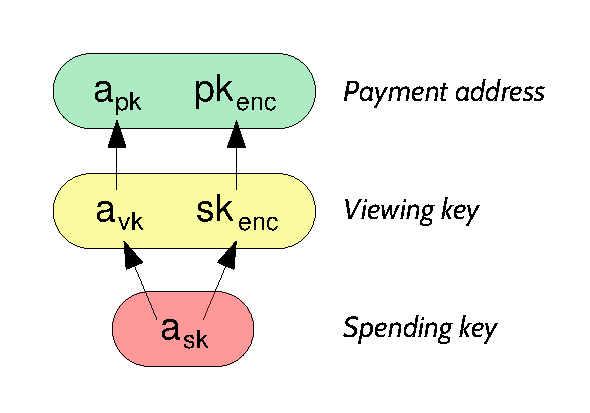
\includegraphics[scale=.7]{key_components}
\end{center}

The derivation of these components is detailed in \crossref{keycomponents}.

\saplingonly{
\todo{Add diagram for diversified keys.}
}

The composition of \paymentAddresses\changed{, \incomingViewingKeys,} and
\spendingKeys is a cryptographic protocol detail that should not normally be
exposed to users. However, user-visible operations should be provided
to obtain a \paymentAddress\changed{ or \incomingViewingKey} from a \spendingKey.

\sproutonly{
Users can accept payment from multiple parties with a single \paymentAddress
$\PaymentAddress$ and the fact that these payments are destined to
the same payee is not revealed on the \blockchain, even to the
paying parties. \emph{However} if two parties collude to compare a
\paymentAddress they can trivially determine they are the same. In the
case that a payee wishes to prevent this they should create a distinct
\paymentAddress for each payer.
}

\pnote{
It is conventional in cryptography to refer to the key used to encrypt
a message in an asymmetric encryption scheme as the ``public key".
However, the public key used as the \transmissionKey component
of an address ($\TransmitPublic$) need not be publically distributed; it
has the same distribution as the \paymentAddress itself. As mentioned above,
limiting the distribution of the \paymentAddress is important for some use cases.
This also helps to reduce reliance of the overall protocol on the security
of the cryptosystem used for \note encryption (see \crossref{inband}), since
an adversary would have to know $\TransmitPublic$ in order to exploit a
hypothetical weakness in that cryptosystem.
}

\introsection
\nsubsection{\Notes}

\saplingonly{
\todo{Update this section.}
}

\sproutonly{
A \note (denoted $\NoteTuple{}$) is a tuple $\changed{(\AuthPublic, \Value,
\NoteAddressRand, \NoteCommitRand)}$. It represents that a value $\Value$ is
spendable by the recipient who holds the \spendingKey $\AuthPrivate$ corresponding
to $\AuthPublic$, as described in the previous section.
}

\begin{itemize}
  \item $\AuthPublic \typecolon \PRFOutput$ is the
        \payingKey of the recipient;
  \item $\Value \typecolon \range{0}{\MAXMONEY}$ is an integer
        representing the value of the \note in \zatoshi
        ($1$ \ZEC = $10^8$ \zatoshi);
  \item $\NoteAddressRand \typecolon \PRFOutput$
        is used as input to $\PRFnf{\AuthPrivate}$ to derive the
        \nullifier of the \note;
  \item $\NoteCommitRand \typecolon \bitseq{\NoteCommitRandLength}$
        is a random bit sequence used as a \commitmentTrapdoor as
        defined in \crossref{abstractcomm}.
\end{itemize}

\sproutonly{
Let $\NoteType$ be the type of a \note, i.e. \changed{
$\PRFOutput \times \range{0}{\MAXMONEY} \times \PRFOutput \times \bitseq{\NoteCommitRandLength}$}.
}

Creation of new \notes is described in \crossref{send}. When \notes are sent,
only a commitment (see \crossref{abstractcomm}) to the above values is disclosed
publically. This allows the value and recipient to be kept private, while the
commitment is used by the \zeroKnowledgeProof when the \note is spent, to check
that it exists on the \blockchain.

The \noteCommitment is computed as
$\NoteCommit(\NoteTuple{}) = \Commit{\NoteCommitRand}(\AuthPublic, \Value, \NoteAddressRand)$,
where $\Commit{}$ is instantiated in \crossref{concretecomm}.

A \nullifier (denoted $\nf$) is derived from the $\NoteAddressRand$ component
of a \note and the recipient's \spendingKey, using a \pseudoRandomFunction (see
\crossref{abstractprfs}). Specifically it is derived as $\PRFnf{\AuthPrivate}(\NoteAddressRand)$
where $\PRFnf{}{}$ is instantiated in \crossref{concreteprfs}.

A \note is spent by proving knowledge of $\NoteAddressRand$ and $\AuthPrivate$ in
zero knowledge while publically disclosing its \nullifier $\nf$, allowing $\nf$ to
be used to prevent double-spending.

\nsubsubsection{\NotePlaintexts{} and \Memos}

Transmitted \notes are stored on the \blockchain in encrypted form, together with
a \noteCommitment $\cm$.

The \notePlaintexts in a \joinSplitDescription are encrypted to the
respective \transmissionKeys $\TransmitPublicNew{\allNew}$,
and the result forms part of a \notesCiphertext (see \crossref{inband}
for further details).

\saplingonly{
\todo{Describe encryption to diversified addresses.}
}

\sproutonly{
Each \notePlaintext (denoted $\NotePlaintext{}$) consists of
$(\Value, \NoteAddressRand, \NoteCommitRand\changed{, \Memo})$.
}

The first three of these fields are as defined earlier.

\changed{
$\Memo$ represents a \memo associated with this \note. The usage of the
\memo is by agreement between the sender and recipient of the \note.
}


\nsubsection{The Block Chain} \label{blockchain}

At a given point in time, each \fullnode is aware of a set of candidate
\blocks. These form a tree rooted at the \genesisBlock, where each node
in the tree refers to its parent via the $\hashPrevBlock$ \blockHeader field
(see \crossref{blockheader}).

A path from the root toward the leaves of the tree consisting of a sequence
of one or valid \blocks consistent with consensus rules, is called a valid
\blockchain.

Each \block in a \blockchain has a \blockHeight. The \blockHeight of the
\genesisBlock is 0, and the \blockHeight of each subsequent \block in the
\blockchain increments by 1.

In order to choose the ``best'' valid \blockchain in its view of the overall
\block tree, a node sums the work, as defined in \crossref{workdef}, of
all \blocks in each chain, and considers the chain with greatest total work
to be best. To break ties between leaf \blocks, a node will prefer the
\block that it received first.

The consensus protocol is designed to ensure that for any given \blockHeight,
the vast majority of nodes should eventually agree on their ``best''
\blockchain up to that height.


\nsubsection{Transactions and Treestates} \label{transactions}

Each \block contains one or more \transactions.

Inputs to a \transaction insert value into a \transparentValuePool, and outputs
remove value from this pool. As in \Bitcoin, the remaining value in the pool is
available to miners as a fee.

\vspace{-3ex}
\consensusrule{
The remaining value in the \transparentValuePool{} \MUST be nonnegative.
}
\vspace{2ex}

To each \transaction there is associated an initial \treestate.

\sproutonly{
A \treestate consists of:
\begin{itemize}
  \item a \noteCommitmentTree (\crossref{merkletree});
  \item a \nullifierSet (\crossref{nullifierset});
  \item data structures associated with \Bitcoin such as the UTXO
        (Unspent Transaction Output) set.
\end{itemize}
}

\saplingonly{
A \treestate consists of:
\begin{itemize}
  \item two \noteCommitmentTrees (\crossref{merkletree});
  \item two \nullifierSets (\crossref{nullifierset});
  \item data structures associated with \Bitcoin such as the UTXO set.
\end{itemize}

One pair of \noteCommitmentTree and \nullifierSet is associated with \Sprout and
the other with \Sapling.
}

An \anchor is a Merkle tree root of a \noteCommitmentTree. It uniquely identifies
a \noteCommitmentTree state given the assumed security properties of the Merkle tree's
hash function. Since the \nullifierSet is always updated together with the
\noteCommitmentTree, this also identifies a particular state of the \nullifierSet.

\introlist
In a given \blockchain, \treestates are chained as follows:

\begin{itemize}
  \item The input \treestate of the first \block is the empty \treestate.
  \item The input \treestate of the first \transaction of a \block is the final
        \treestate of the immediately preceding \block.
  \item The input \treestate of each subsequent \transaction in a \block is the
        output \treestate of the immediately preceding \transaction.
  \item The final \treestate of a \block is the output \treestate of its last
        \transaction.
\end{itemize}

\joinSplitDescriptions also have interstitial input and output \treestates, explained
in the following section.


\nsubsection{\JoinSplitTransfers{} and Descriptions} \label{joinsplit}

A \joinSplitDescription is data included in a \transaction that describes a \joinSplitTransfer,
i.e.\ a \shielded value transfer. This kind of value transfer is the primary
\Zcash-specific operation performed by \transactions; it uses, but should not be
confused with, the \joinSplitStatement used for the \zkSNARK proof and verification.

A \joinSplitTransfer spends $\NOld$ \notes $\nOld{\allOld}$ and \transparent input
$\vpubOld$, and creates $\NNew$ \notes $\nNew{\allNew}$ and \transparent output
$\vpubNew$.

Each \transaction is associated with a \sequenceOfJoinSplitDescriptions.

The \changed{total $\vpubNew$ value adds to, and the total} $\vpubOld$
value subtracts from the \transparentValuePool of the containing \transaction.

The \anchor of each \joinSplitDescription in a \transaction{} refers to a
\treestate. For the first \joinSplitDescription, this \MUST be the output
\treestate of a previous \block.

\changed{
For each \joinSplitDescription in a \transaction, an interstitial output \treestate is
constructed which adds the \noteCommitments and \nullifiers specified in that
\joinSplitDescription to the input \treestate referred to by its \anchor.
This interstitial output \treestate is available for use as the \anchor of subsequent
\joinSplitDescriptions in the same \transaction.

Interstitial \treestates are necessary because when a \transaction is constructed,
it is not known where it will eventually appear in a mined \block. Therefore the
\anchors that it uses must be independent of its eventual position.
}

\begin{consensusrules}
  \item The input and output values of each \joinSplitTransfer{} \MUST balance
        exactly.
\changed{
  \item The \anchor of each \joinSplitDescription in a \transaction{} \MUST refer
        to either some earlier \block's final \treestate, or to the interstitial output
        \treestate of any prior \joinSplitDescription in the same \transaction.
}
\end{consensusrules}

\nsubsection{\NoteCommitmentTrees} \label{merkletree}

\begin{center}
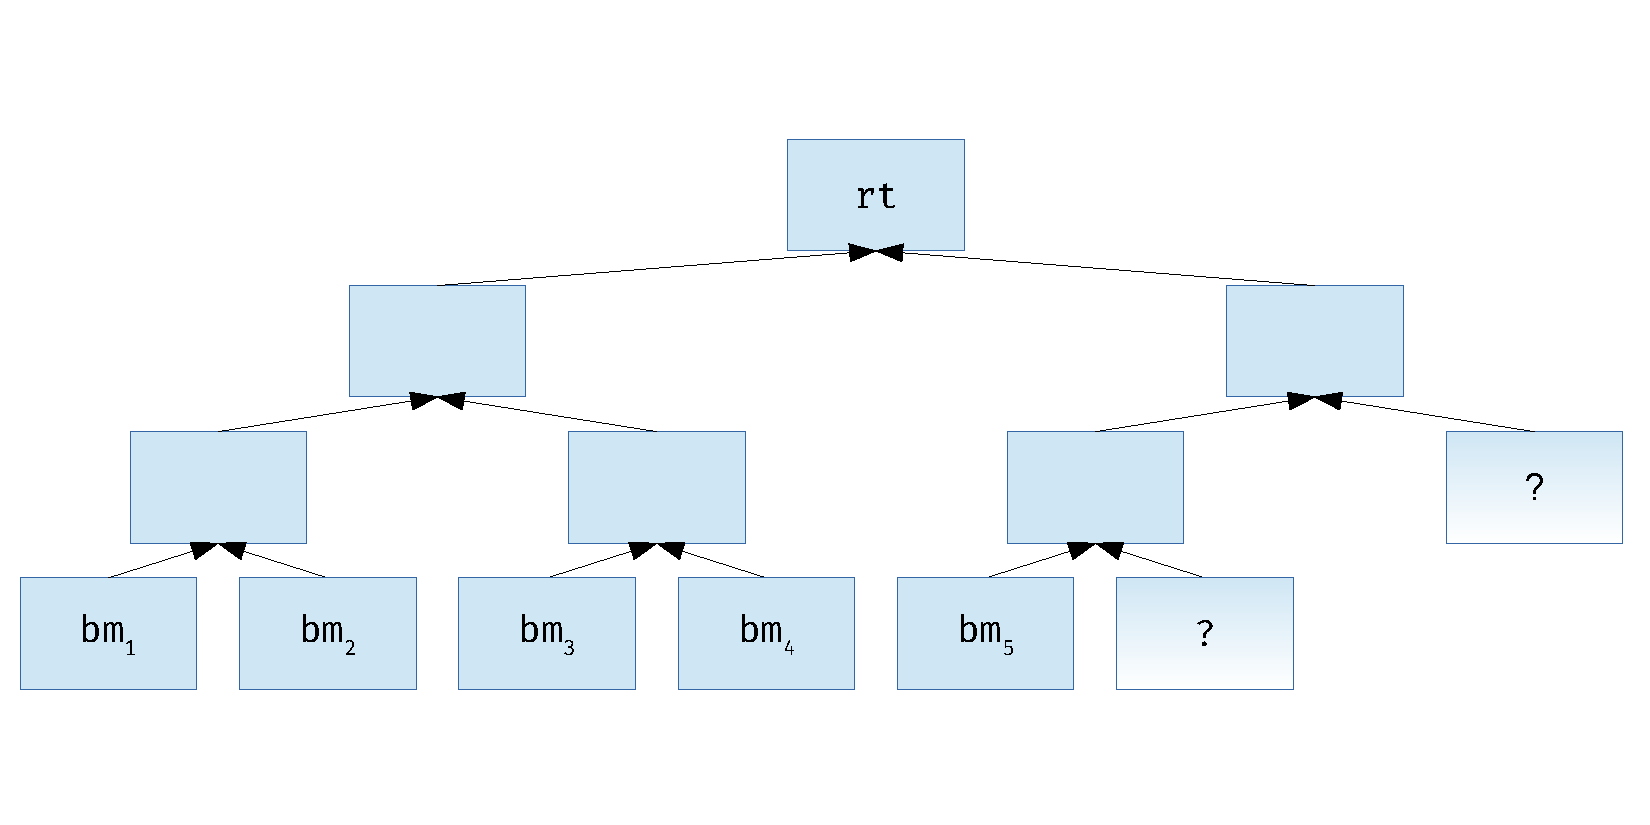
\includegraphics[scale=.4]{incremental_merkle}
\end{center}

The \noteCommitmentTree is an \incrementalMerkleTree of fixed depth used to
store \noteCommitments that \joinSplitTransfers produce. Just as the \term{unspent
transaction output set} (UTXO set) used in \Bitcoin, it is used to express the existence
of value and the capability to spend it. However, unlike the UTXO set, it is \emph{not}
the job of this tree to protect against double-spending, as it is append-only.

A \merkleRoot of this tree is associated with each \treestate, as described in
\crossref{transactions}.

Each \merkleNode in the \incrementalMerkleTree is associated with a \merkleHash of
size $\MerkleHashLength$ bits.
The \merkleLayer numbered $h$, counting from \merkleLayer $0$ at the \merkleRoot, has
$2^h$ \merkleNodes with \merkleIndices $0$ to $2^h-1$ inclusive.
The \merkleHash associated with the \merkleNode at \merkleIndex $i$ in \merkleLayer $h$
is denoted $\MerkleNode{h}{i}$.


\nsubsection{\NullifierSets} \label{nullifierset}

Each \fullnode maintains a \nullifierSet logically associated with each \treestate.
As valid \transactions containing \joinSplitTransfers are processed, the \nullifiers
revealed in \joinSplitDescriptions are inserted into this \nullifierSet.

\xNullifiers are enforced to be unique within a valid \blockchain, in order to
prevent double-spends.

\consensusrule{
A \nullifier{} \MUSTNOT repeat either within a \transaction, or across
\transactions in a valid \blockchain.
}

\sapling{\pnote{
\Sprout and \Sapling \nullifiers are considered disjoint, even if they have
the same bit pattern.
}}


\nsubsection{Block Subsidy and Founders' Reward} \label{subsidyconcepts}

Like \Bitcoin, \Zcash creates currency when \blocks are mined. The value created on
mining a \block is called the \blockSubsidy. It is composed of a \minerSubsidy and a
\foundersReward. As in \Bitcoin, the miner of a \block also receives \transactionFees.

The calculations of the \blockSubsidy, \minerSubsidy, and \foundersReward depend on
the \blockHeight, as defined in \crossref{blockchain}.

These calculations are described in \crossref{subsidies}.


\nsubsection{\CoinbaseTransactions}

The first \transaction in a block must be a \coinbaseTransaction, which should
collect and spend any \minerSubsidy and \transactionFees paid by \transactions
included in this \block. The \coinbaseTransaction must also pay the \foundersReward
as described in \crossref{foundersreward}.


\nsection{Abstract Protocol}

\nsubsection{Abstract Cryptographic Schemes}

\nsubsubsection{Hash Functions} \label{abstracthashes}

$\MerkleCRH \typecolon \MerkleHash \times \MerkleHash \rightarrow \MerkleHash$
is a collision-resistant hash function used in \crossref{merklepath}.
It is instantiated in \crossref{merklecrh}.

\changed{
$\hSigCRH{} \typecolon \bitseq{\RandomSeedLength} \times \typeexp{\PRFOutput}{\NOld} \times \JoinSplitSigPublic \rightarrow \hSigType$
is a collision-resistant hash function used in \crossref{joinsplitdesc}.
It is instantiated in \crossref{hsigcrh}.

$\EquihashGen{} \typecolon (n \typecolon \PosInt) \times \PosInt \times \byteseqs \times \PosInt \rightarrow \bitseq{n}$
is another hash function, used in \crossref{equihash} to generate
input to the Equihash solver. The first two arguments, representing
the Equihash parameters $n$ and $k$, are written subscripted.
It is instantiated in \crossref{equihashgen}.
}

\introlist
\nsubsubsection{\PseudoRandomFunctions} \label{abstractprfs}

$\PRF{x}{}$ is a \pseudoRandomFunction keyed by $x$. \changed{Four} \emph{independent}
$\PRF{x}{}$ are needed in our protocol:

\begin{tabular}{@{\hskip 2em}l@{\;}l@{\;}l@{\;}l@{\;}l}
$\PRFaddr{} $&$\typecolon\; \bitseq{\AuthPrivateLength} $&$\times\; \range{0}{255} $& &$\rightarrow \PRFOutput $\\
$\PRFnf{}   $&$\typecolon\; \bitseq{\AuthPrivateLength} $&$\times\; \PRFOutput $& &$\rightarrow \PRFOutput $\\
$\PRFpk{}   $&$\typecolon\; \bitseq{\AuthPrivateLength} $&$\times\; \setofOld $&$\times\; \hSigType $&$\rightarrow \PRFOutput $\\
$\PRFrho{}  $&$\typecolon\; \bitseq{\NoteAddressPreRandLength} $&$\times\; \setofNew $&$\times\; \hSigType $&$\rightarrow \PRFOutput $
\end{tabular}

These are used in \crossref{sproutstatement}; $\PRFaddr{}$ is also used to
derive a \paymentAddress from a \spendingKey in \crossref{keycomponents}.

They are instantiated in \crossref{concreteprfs}.

\securityrequirement{
In addition to being \pseudoRandomFunctions, it is required that $\PRFnf{x}$
\changed{, $\PRFaddr{x}$, and $\PRFrho{x}$} be collision-resistant across all $x$ ---
i.e.\ it should not be feasible to find $(x, y) \neq (x', y')$ such that
$\PRFnf{x}(y) = \PRFnf{x'}(y')$\changed{, and similarly for $\PRFaddr{}$ and $\PRFrho{}$}.
}

\pnote{$\PRFnf{}$ was called $\PRFsn{}$ in \Zerocash \cite{BCG+2014}.}

\nsubsubsection{\SymmetricEncryption} \label{abstractsym}

Let $\Sym$ be an \symmetricEncryptionScheme with keyspace $\Keyspace$, encrypting
plaintexts in $\Plaintext$ to produce ciphertexts in $\Ciphertext$.

$\SymEncrypt{} \typecolon \Keyspace \times \Plaintext \rightarrow \Ciphertext$
is the encryption algorithm.

$\SymDecrypt{} \typecolon \Keyspace \times \Ciphertext \rightarrow
\Plaintext \union \setof{\bot}$ is the corresponding decryption algorithm, such that
for any $\Key \in \Keyspace$ and $\Ptext \in \Plaintext$,
$\SymDecrypt{\Key}(\SymEncrypt{\Key}(\Ptext)) = \Ptext$.
$\bot$ is used to represent the decryption of an invalid ciphertext.

\securityrequirement{
$\Sym$ must be one-time (INT-CTXT $\wedge$ IND-CPA)-secure. ``One-time'' here means
that an honest protocol participant will almost surely encrypt only one message with
a given key; however, the attacker may make many adaptive chosen ciphertext queries
for a given key. The security notions INT-CTXT and IND-CPA are as defined in
\cite{BN2007}.
}

\nsubsubsection{\KeyAgreement} \label{abstractkeyagreement}

A \keyAgreementScheme is a cryptographic protocol in which two parties agree
a shared secret, each using their private key and the other party's public key.

A \keyAgreementScheme $\KA$ defines a type of public keys $\KAPublic$, a type
of private keys $\KAPrivate$, and a type of shared secrets $\KASharedSecret$.

Let $\KAFormatPrivate \typecolon \PRFOutput \rightarrow \KAPrivate$ be a function
that converts a bit string of length $\PRFOutputLength$ to a $\KA$ private key.

Let $\KADerivePublic \typecolon \KAPrivate \rightarrow \KAPublic$ be a function
that derives the $\KA$ public key corresponding to a given $\KA$ private key.

Let $\KAAgree \typecolon \KAPrivate \times \KAPublic \rightarrow \KASharedSecret$
be the agreement function.

\pnote{
The range of $\KADerivePublic$ may be a strict subset of $\KAPublic$.
}

\begin{securityrequirements}
  \item $\KAFormatPrivate$ must preserve sufficient entropy from its input to be used
        as a secure $\KA$ private key.
  \item The key agreement and the KDF defined in the next section must together
        satisfy a suitable adaptive security assumption along the lines of
        \cite[section 3]{Bern2006} or \cite[Definition 3]{ABR1999}.
\end{securityrequirements}

More precise formalization of these requirements is beyond the scope of this
specification.


\nsubsubsection{\KeyDerivation} \label{abstractkdf}

A \keyDerivationFunction is defined for a particular \keyAgreementScheme and
\symmetricEncryptionScheme; it takes the shared secret produced by the key
agreement and additional arguments, and derives a key suitable for the encryption
scheme.

Let $\KDF \typecolon \setofNew \times \hSigType \times \KASharedSecret
\times \KAPublic \times \KAPublic \rightarrow \Keyspace$ be a
\keyDerivationFunction suitable for use with $\KA$, deriving keys
for $\SymEncrypt{}$.

\securityrequirement{
In addition to adaptive security of the key agreement and KDF,
the following security property is required:

Let $\TransmitPrivateSup{1}$ and $\TransmitPrivateSup{2}$ each be chosen uniformly and
independently at random from $\KAPrivate$.

Let $\TransmitPublicSup{j} := \KADerivePublic(\TransmitPrivateSup{j})$.

\introlist
An adversary can adaptively query a function
$Q \typecolon \range{1}{2} \times \hSigType \rightarrow
\KAPublic \times \Keyspace_{\allNew}$ where $Q_j(\hSig)$ is defined as follows:
\begin{enumerate}
  \item Choose $\EphemeralPrivate$ uniformly at random from $\KAPrivate$.
  \item Let $\EphemeralPublic := \KADerivePublic(\EphemeralPrivate)$.
  \item For $i \in \setofNew$, let $\Key_i :=
        \KDF(i, \hSig, \KAAgree(\EphemeralPrivate, \TransmitPublicSup{j}), \EphemeralPublic, \TransmitPublicSup{j}))$.
  \item Return $(\EphemeralPublic, \Key_{\allNew})$.
\end{enumerate}

Then the adversary must make another query to $Q_j$ with random unknown
$j \in \range{1}{2}$, and guess $j$ with probability greater than chance.
}

If the adversary's advantage is negligible, then the asymmetric encryption scheme
constructed from $\KA$, $\KDF$ and $\Sym$ in \crossref{inband} will be key-private
as defined in \cite{BBDP2001}.

\pnote{
The given definition only requires ciphertexts to be indistinguishable
between \transmissionKeys that are outputs of $\KADerivePublic$ (which
includes all keys generated as in \crossref{keycomponents}). If a
\transmissionKey not in that range is used, it may be distinguishable.
This is not considered to be a significant security weakness.
}


\introlist
\nsubsubsection{Signature} \label{abstractsig}

A signature scheme $\Sig$ defines:

\begin{itemize}
  \item a type of signing keys $\SigPrivate$;
  \item a type of verifying keys $\SigPublic$;
  \item a type of messages $\SigMessage$;
  \item a type of signatures $\SigSignature$;
  \item a randomized key pair generation algorithm $\SigGen \typecolon () \rightarrowR \SigPrivate \times \SigPublic$;
  \item a randomized signing algorithm $\SigSign{} \typecolon \SigPrivate \times \SigMessage \rightarrowR \SigSignature$;
  \item a verifying algorithm $\SigVerify{} \typecolon \SigPublic \times \SigMessage \times \SigSignature \rightarrow \bit$;
\end{itemize}

such that for any key pair $(\sk, \vk) \leftarrowR \SigGen()$, and
any $m \typecolon \SigMessage$ and $s \typecolon \SigSignature \leftarrowR \SigSign{\sk}(m)$,
$\SigVerify{\vk}(m, s) = 1$.

\Zcash uses two signature schemes, one used for signatures that can be verified
by script operations such as \ScriptOP{CHECKSIG} and \ScriptOP{CHECKMULTISIG} as
in \Bitcoin, and one called $\JoinSplitSig$ which is used to sign \transactions
that contain at least one \joinSplitDescription. The latter is instantiated in
\crossref{concretesig}. The following defines only the security properties needed
for $\JoinSplitSig$.

\securityrequirement{
$\JoinSplitSig$ must be Strongly Unforgeable under (non-adaptive)
Chosen Message Attack (SU-CMA), as defined for example in
\cite[Definition 6]{BDEHR2011}. This allows an adversary to obtain
signatures on chosen messages, and then requires it to be infeasible
for the adversary to forge a previously unseen valid \mbox{(message, signature)}
pair without access to the signing key.
}

\begin{pnotes}
  \item Since a fresh key pair is generated for every \transaction containing
        a \joinSplitDescription and is only used for one signature (see
        \crossref{nonmalleability}), a one-time signature scheme would
        suffice for $\JoinSplitSig$. This is also the reason why only
        security against \emph{non-adaptive} chosen message attack is needed.
        In fact the instantiation of $\JoinSplitSig$ uses a scheme designed
        for security under adaptive attack even when multiple signatures are
        signed under the same key.
  \item SU-CMA security requires it to be infeasible for the adversary, not
        knowing the private key, to forge a distinct signature on a previously
        seen message. That is, \joinSplitSignatures are intended to be
        nonmalleable in the sense of \cite{BIP-62}.
\end{pnotes}


\introlist
\nsubsubsection{Commitment} \label{abstractcomm}

A \commitmentScheme is a function that, given a random \commitmentTrapdoor
and an input, can be used to commit to the input in such a way that:

\begin{itemize}
  \item no information is revealed about it without the \trapdoor (``hiding''),
  \item given the \trapdoor and input, the commitment can be verified to ``open''
        to that input and no other (``binding'').
\end{itemize}

\vspace{-3ex}
A \commitmentScheme $\Commit{}$ defines a type of inputs $\CommitInput$,
a type of commitments $\CommitOutput$, and a type of \commitmentTrapdoors
$\CommitTrapdoor$.

Let $\Commit{} \typecolon \CommitTrapdoor \times \CommitInput \rightarrow \CommitOutput$
be a function satisfying the security requirements below.

\begin{securityrequirements}
  \item \textbf{Computational hiding:} For all $x, x' \typecolon \CommitInput$,
        the distributions $\{\; \Commit{r}(x) \;|\; r \leftarrowR \CommitTrapdoor \;\}$
        and $\{\; \Commit{r}(x') \;|\; r \leftarrowR \CommitTrapdoor \;\}$ are
        computationally indistinguishable.
  \item \textbf{Computational binding:} It is infeasible to find
        $x, x' \typecolon \CommitInput$ and
        $r, r' \typecolon \CommitTrapdoor$
        such that $x \neq x'$ and $\Commit{r}(x) = \Commit{r'}(x')$.
\end{securityrequirements}


\introlist
\nsubsubsection{\RepresentedGroup} \label{abstractgroup}

A \representedGroup $\GroupG{}$ consists of:

\begin{itemize}
  \item a subgroup order parameter $\ParamG{r} \typecolon \PosInt$, which must be prime;
  \item a cofactor parameter $\ParamG{h} \typecolon \PosInt$;
  \item a group $\GroupG{}$ of order $\ParamG{h} \mult \ParamG{r}$, written additively
        with operation $+ \typecolon \GroupG{} \times \GroupG{} \rightarrow \GroupG{}$,
        and additive identity $\ZeroG{}$;
  \item a generator $\GenG{}$ of the subgroup of $\GroupG{}$ of order $\ParamG{r}$;
  \item a bit-length parameter $\ellG{} \typecolon \Nat$;
  \item a representation function $\repr_{\GroupG{}} \typecolon
        \GroupG{} \rightarrow \bitseq{\ellG{}}$;
  \item an abstraction function $\abst_{\GroupG{}} \typecolon
        \bitseq{\ellG{}} \rightarrow \GroupG{} \union \setof{\bot}$;
\end{itemize}
\vspace{-2ex}
such that $\abst_{\GroupG{}}$ is the left inverse of $\repr_{\GroupG{}}$, i.e.
for all $P \in \GroupG{}$, $\abst_{\GroupG{}}(\repr_{\GroupG{}}(P)) = P$, and
for all $S$ not in the image of $\repr_{\GroupG{}}$, $\abst_{\GroupG{}}(S) = \bot$.

We extend the $\vsum{}{}$ notation to addition on group elements.

\vspace{-3ex}
For $G \typecolon \GroupG{}$ and $s \typecolon \Nat$ (or $s \typecolon \GF{\ParamG{r}}$)
we write $\scalarmult{s}{G}$ for $\vsum{i = 1}{s} G$.
\vspace{1ex}


\sapling{
\introlist
\nsubsubsection{\HashExtractor} \label{abstractextractor}

A \hashExtractor for a \representedGroup $\GroupG{}$ is a function
$\ExtractG \typecolon \GroupG{} \rightarrow \bitseq{\ell}$ for some $\ell \typecolon \Nat$,
such that $\ExtractG$ is injective on the subgroup generated by $\GenG{}$.

\pnote{
Unlike the representation function $\repr_{\GroupG{}}$, $\ExtractG$ need not have an
efficiently computable left inverse.
}
}


\sapling{
\introlist
\nsubsubsection{\GroupHash} \label{abstractgrouphash}

Given a represented group $\GroupG{}$ and a type $\Index$, a
\term{family of group hashes into $\GroupG{}$} is a function
$\GroupGHash{} \typecolon \Index \times \bitseq{\ell} \rightarrow \GroupG{}$.

\begin{securityrequirements}
  \item \textbf{Discrete Logarithm Independence:} For a randomly selected member
$\GroupGHash{U}$ of the family, it is infeasible to find
a sequence of distinct inputs $m_{\alln} \typecolon \typeexp{\bitseq{\ell}}{n}$
and a sequence of nonzero scalars $x_{\alln} \typecolon \typeexp{\GFstar{\ParamG{r}}}{n}$
such that $\vsum{i = 1}{n}(\scalarmult{x_i}{\GroupGHash{U}(m_i)}) = \ZeroG{}$.
\end{securityrequirements}

Note that this property implies (and is stronger than) collision-resistance,
since a collision $(m_1, m_2)$ for $\GroupGHash{U}$ trivially gives a discrete
logarithm relation with $x_1 = 1$ and $x_2 = -1$.
}

\introlist
\nsubsubsection{\RepresentedPairing} \label{abstractpairing}

A \representedPairing $\GroupP{}$ consists of:

\begin{itemize}
  \item a group order parameter $\ParamP{r} \typecolon \PosInt$ which must be prime;
  \item two \representedGroups $\GroupP{1..2}$, both of order $\ParamP{r}$;
  \item a group $\GroupP{T}$ of order $\ParamP{r}$, written multiplicatively with operation
        $\mult \typecolon \GroupP{T} \times \GroupP{T} \rightarrow \GroupP{T}$
        and multiplicative identity $\ParamP{\mathbf{1}}$;
  \item a pairing function
        $\PairingP \typecolon \GroupP{1} \times \GroupP{2} \rightarrow \GroupP{T}$
        satisfying:

        \begin{itemize}
          \item (Bilinearity)\; for all $a, b \typecolon \GFstar{r}$,
                $P \typecolon \GroupP{1}$, and $Q \typecolon \GroupP{2}$,
                $\PairingP(\scalarmult{a}{P}, \scalarmult{b}{Q}) = \PairingP(P, Q)^{a \mult b}$, and
          \item (Nondegeneracy)\; there does not exist $P \typecolon \GroupP{1} \setminus \ZeroP{1}$
                such that for all $Q \typecolon \GroupP{2},
                \PairingP(P, Q) = \ParamP{\mathbf{1}}$;
        \end{itemize}
\end{itemize}

\nsubsubsection{\ZeroKnowledgeProvingSystem} \label{abstractzk}

A \zeroKnowledgeProvingSystem is a cryptographic protocol that allows
proving a particular \statement, dependent on \primary and \auxiliaryInputs,
in zero knowledge --- that is, without revealing information about the
\auxiliaryInputs other than that implied by the \statement. The type of
\zeroKnowledgeProvingSystem needed by \Zcash is a \ppzkSNARK.

\introlist
A \ppzkSNARK instance $\ZK$ defines:

\begin{itemize}
  \item a type of \zkProvingKeys, $\ZKProvingKey$;
  \item a type of \zkVerifyingKeys, $\ZKVerifyingKey$;
  \item a type of \primaryInputs $\ZKPrimary$;
  \item a type of \auxiliaryInputs $\ZKAuxiliary$;
  \item a type of proofs $\ZKProof$;
  \item a type $\ZKSatisfying \subseteq \ZKPrimary \times \ZKAuxiliary$ of inputs satisfying
the \statement;
  \item a randomized key pair generation algorithm $\ZKGen \typecolon () \rightarrowR \ZKProvingKey \times \ZKVerifyingKey$;
  \item a proving algorithm $\ZKProve{} \typecolon \ZKProvingKey \times \ZKSatisfying \rightarrow \ZKProof$;
  \item a verifying algorithm $\ZKVerify{} \typecolon \ZKVerifyingKey \times \ZKPrimary \times \ZKProof \rightarrow \bit$;
\end{itemize}

The security requirements below are supposed to hold with overwhelming
probability for $(\pk, \vk) \leftarrowR \ZKGen()$.

\begin{securityrequirements}
  \item \textbf{Completeness:} An honestly generated proof will convince a verifier:
for any $(x, w) \in \ZKSatisfying$, if $\ZKProve{\pk}(x, w)$ outputs $\Proof{}$,
then $\ZKVerify{\vk}(x, \Proof{}) = 1$.
  \item \textbf{Knowledge Soundness:} For any adversary $\Adversary$ able to find an
$x \typecolon \ZKPrimary$ and proof $\Proof{} \typecolon \ZKProof$ such that $\ZKVerify{\vk}(x, \Proof{}) = 1$,
there is an efficient extractor $E_{\Adversary}$ such that if $E_{\Adversary}(\vk, \pk)$
returns $w$, then the probability that $(x, w) \not\in \ZKSatisfying$ is negligable.
  \item \textbf{Statistical Zero Knowledge:} An honestly generated proof is statistical
zero knowledge. That is, there is a feasible stateful simulator $\Simulator$ such that,
for all stateful distinguishers $\Distinguisher$, the following two probabilities are
negligibly close:
\vspace{0.5ex}

$\;\;\Prob{
  (x, w) \in \ZKSatisfying \\
  \Distinguisher(\Proof{}) = 1
}{
  (\pk, \vk) \leftarrowR \ZKGen() \\
  (x, w) \leftarrowR \Distinguisher(\pk, \vk) \\
  \Proof{} \leftarrowR \ZKProve{\pk}(x, w)
}
\text{\; and \;}
\Prob{
  (x, w) \in \ZKSatisfying \\
  \Distinguisher(\Proof{}) = 1
}{
  (\pk, \vk) \leftarrowR \Simulator() \\
  (x, w) \leftarrowR \Distinguisher(\pk, \vk) \\
  \Proof{} \leftarrowR \Simulator(x)
}$
\end{securityrequirements}

These definitions are derived from those in \cite[Appendix C]{BCTV2014}, adapted to
state concrete security for a fixed circuit, rather than asymptotic security for
arbitrary circuits. ($\ZKProve{}$ corresponds to $P$, $\ZKVerify{}$ corresponds to $V$,
and $\ZKSatisfying$ corresponds to $\mathcal{R}_C$ in the notation of that appendix.)

The Knowledge Soundness definition is a way to formalize the property that it is
infeasible to find a new proof $\Proof{}$ where $\ZKVerify{\vk}(x, \Proof{}) = 1$ without
\emph{knowing} an \auxiliaryInput $w$ such that $(x, w) \in \ZKSatisfying$.
Note that Knowledge Soundness implies Soundness --- i.e.\ the property that it is
infeasible to find a new proof $\Proof{}$ where $\ZKVerify{\vk}(x, \Proof{}) = 1$ without
\emph{there existing} an \auxiliaryInput $w$ such that $(x, w) \in \ZKSatisfying$.

It is possible to replay proofs, but informally, a proof for a given $(x, w)$ gives
no information that helps to find a proof for other $(x, w)$.

\sprout{
The \provingSystem is instantiated in \crossref{phgr}.
$\SproutJoinSplit$ refers to this \provingSystem with the $\BNCurve$ pairing,
specialized to the \joinSplitStatement given in \crossref{sproutstatement}.
In this case we omit the key subscripts on $\SproutJoinSplitProve$ and $\SproutJoinSplitVerify$,
taking them to be the particular \provingKey and \verifyingKey defined by the
\joinSplitParameters in \crossref{sproutparameters}.
}
\sapling{
\Zcash uses two \provingSystems:
\begin{itemize}
  \item $\PHGR$ (\crossref{phgr}) is used with the
        $\BNCurve$ pairing (\crossref{bnpairing}),
        to prove and verify the \Sprout \joinSplitStatement
        (\crossref{sproutstatement}).
  \item $\Groth$ (\crossref{groth}) is used with the
        $\BLSCurve$ pairing (\crossref{blspairing}),
        to prove and verify the \Sapling \spendStatement
        (\crossref{saplingstatement}) \todo{and maybe other statements}.
\end{itemize}

These specializations are referred to as
$\SproutJoinSplit$ and $\SaplingSpend$ respectively.

We omit the key subscripts on $\SproutJoinSplitProve$ and
$\SproutJoinSplitVerify$, taking them to be the \Sprout \provingKey
and \verifyingKey defined in \crossref{sproutparameters}.

Similarly, we omit the key subscripts on $\SaplingSpendProve$
and $\SaplingSpendVerify$, taking them to be the \Sapling \provingKey
and \verifyingKey defined in \crossref{saplingparameters}.

See \crossref{saplingtransition} for further details on the
usage of each of these schemes.
}

\nsubsection{Key Components} \label{keycomponents}

Let $\PRFaddr{}$ be a \pseudoRandomFunction, instantiated in \crossref{concreteprfs}.

Let $\KA$ be a \keyAgreementScheme, instantiated in \crossref{concretekeyagreement}.

A new \spendingKey $\AuthPrivate$ is generated by choosing a bit string
uniformly at random from $\bitseq{\AuthPrivateLength}$.

\introlist
\changed{
$\AuthPublic$, $\TransmitPrivate$ and $\TransmitPublic$ are derived from
$\AuthPrivate$
as follows:}

\begin{tabular}{@{\hskip 2em}r@{\;}l}
  $\AuthPublic$ &$:= \changed{\PRFaddr{\AuthPrivate}(0)}$ \\
  $\TransmitPrivate$ &$:= \changed{\KAFormatPrivate(\PRFaddr{\AuthPrivate}(1))}$ \\
  $\TransmitPublic$ &$:= \changed{\KADerivePublic(\TransmitPrivate)}$.
\end{tabular}

\nsubsection{\JoinSplitDescriptions} \label{joinsplitdesc}

A \joinSplitTransfer, as specified in \crossref{joinsplit}, is encoded in
\transactions as a \joinSplitDescription.

Each \transaction includes a sequence of zero or more \joinSplitDescriptions.
When this sequence is non-empty, the \transaction also includes encodings of a
$\JoinSplitSig$ public verification key and signature.

\introlist
Each \joinSplitDescription consists of $(\vpubOld, \vpubNew, \rt,
\nfOld{\allOld}, \cmNew{\allNew}, \EphemeralPublic, \RandomSeed,
\h{\allOld}, \ProofSproutJoinSplit, \TransmitCiphertext{\allNew})$

where
\begin{itemize}
  \item \changed{$\vpubOld \typecolon \range{0}{\MAXMONEY}$ is
        the value that the \joinSplitTransfer removes from the \transparentValuePool};
  \item $\vpubNew \typecolon \range{0}{\MAXMONEY}$ is
        the value that the \joinSplitTransfer inserts into the \transparentValuePool;
  \item $\rt \typecolon \MerkleHash$ is an \anchor, as defined in
        \crossref{blockchain}, for the output \treestate of either
        a previous \block, or a previous \joinSplitTransfer in this
        \transaction.
  \item $\nfOld{\allOld} \typecolon \typeexp{\PRFOutput}{\NOld}$ is
        the sequence of \nullifiers for the input \notes;
  \item $\cmNew{\allNew} \typecolon \typeexp{\CommitOutput}{\NNew}$ is
        the sequence of \noteCommitments for the output \notes;
  \item \changed{$\EphemeralPublic \typecolon \KAPublic$ is
        a key agreement public key, used to derive the key for encryption
        of the \notesCiphertext (\crossref{inband})};
  \item \changed{$\RandomSeed \typecolon \RandomSeedType$ is
        a seed that must be chosen independently at random for each
        \joinSplitDescription};
  \item $\h{\allOld} \typecolon \typeexp{\PRFOutput}{\NOld}$ is
        a sequence of tags that bind $\hSig$ to each
        $\AuthPrivate$ of the input \notes;
  \item $\ProofSproutJoinSplit \typecolon \SproutJoinSplitProof$ is
        the \zeroKnowledgeProof for the \joinSplitStatement;
  \item $\TransmitCiphertext{\allNew} \typecolon \typeexp{\Ciphertext}{\NNew}$ is
        a sequence of ciphertext components for the encrypted output \notes.
\end{itemize}

The $\ephemeralKey$ and $\encCiphertexts$ fields together form the \notesCiphertext.

\introlist
The value $\hSig$ is also computed from \changed{$\RandomSeed$, $\nfOld{\allOld}$, and} the
$\joinSplitPubKey$ of the containing \transaction:

\begin{formulae}
  \item $\hSig := \hSigCRH(\changed{\RandomSeed, \nfOld{\allOld},\,} \joinSplitPubKey)$.
\end{formulae}

$\hSigCRH$ is instantiated in \crossref{hsigcrh}.

\begin{consensusrules}
  \item Elements of a \joinSplitDescription{} \MUST have the types given
        above (for example: $0 \leq \vpubOld \leq \MAXMONEY$ and $0 \leq \vpubNew \leq \MAXMONEY$).
  \item Either $\vpubOld$ or $\vpubNew$ \MUST be zero.
  \item The proof $\Proof{\JoinSplit}$ \MUST be valid given a \primaryInput formed
        from the other fields and $\hSig$.
        I.e. it must be the case that $\SproutJoinSplitVerify{}((\rt, \nfOld{\allOld}, \cmNew{\allNew},
        \vpubOld, \vpubNew, \hSig, \h{\allOld}), \Proof{\JoinSplit}) = 1$.
\end{consensusrules}

\introlist
\nsubsection{Sending \Notes} \label{send}

In order to send \shielded value, the sender constructs a \transaction
containing one or more \joinSplitDescriptions. This involves first generating
a new $\JoinSplitSig$ key pair:

\begin{formulae}
  \item $(\joinSplitPrivKey, \joinSplitPubKey) \leftarrowR \JoinSplitSigGen()$.
\end{formulae}

\introlist
For each \joinSplitDescription, the sender chooses $\RandomSeed$ uniformly at
random on $\bitseq{\RandomSeedLength}$, and selects
the input \notes. At this point there is sufficient information to compute $\hSig$,
as described in the previous section. \changed{The sender also chooses $\NoteAddressPreRand$
uniformly at random on $\bitseq{\NoteAddressPreRandLength}$.}
Then it creates each output \note with index $i \typecolon \setofNew$ as follows:

\begin{itemize}
  \item Choose $\NoteCommitRandNew{i}$ uniformly at random on $\bitseq{\NoteCommitRandLength}$.
\changed{
  \item Compute $\NoteAddressRandNew{i} := \PRFrho{\NoteAddressPreRand}(i, \hSig)$.
}
  \item Encrypt the \note to the recipient \transmissionKey $\TransmitPublicNew{i}$,
        as described in \crossref{inband}, giving the ciphertext component
        $\TransmitCiphertext{i}$.
\end{itemize}

In order to minimize information leakage, the sender \SHOULD randomize the order
of the input \notes and of the output \notes. Other considerations relating to
information leakage from the structure of \transactions are beyond the
scope of this specification.

\introlist
After generating all of the \joinSplitDescriptions, the sender obtains the
$\dataToBeSigned$ (\crossref{nonmalleability}), and signs it with
the private \joinSplitSigningKey:

\begin{formulae}
  \item $\joinSplitSig \leftarrowR \JoinSplitSigSign{\text{\small\joinSplitPrivKey}}(\dataToBeSigned)$
\end{formulae}

Then the encoded \transaction including $\joinSplitSig$ is submitted to the network.


\nsubsubsection{\DummyNotes} \label{dummynotes}

The fields in a \joinSplitDescription allow for $\NOld$ input \notes, and
$\NNew$ output \notes. In practice, we may wish to encode a \joinSplitTransfer
with fewer input or output \notes. This is achieved using \dummyNotes.

\introlist
\changed{
A \dummy input \note, with index $i$ in the \joinSplitDescription, is constructed
as follows:

\begin{itemize}
  \item Generate a new random \spendingKey $\AuthPrivateOld{i}$ and derive its
        \payingKey $\AuthPublicOld{i}$.
  \item Set $\vOld{i} := 0$.
  \item Choose $\NoteAddressRandOld{i}$ uniformly at random on $\PRFOutput$.
  \item Choose $\NoteCommitRandOld{i}$ uniformly at random on $\bitseq{\NoteCommitRandLength}$.
  \item Compute $\nfOld{i} := \PRFnf{\AuthPrivateOld{i}}(\NoteAddressRandOld{i})$.
  \item Construct a \dummy \merklePath $\treepath{i}$ for use in the
        \auxiliaryInput to the \joinSplitStatement (this will not be checked).
  \item When generating the \joinSplitProof\!\!, set $\EnforceMerklePath{i}$ to $0$.
\end{itemize}
}

A \dummy output \note is constructed as normal but with zero value, and
sent to a random \paymentAddress.


\nsubsection{Merkle path validity} \label{merklepath}

The depth of the \noteCommitmentTree is $\MerkleDepth$ (defined in \crossref{constants}).

Each \merkleNode in the \incrementalMerkleTree is associated with a \merkleHash,
which is a byte sequence. The \merkleLayer numbered $h$, counting from
\merkleLayer $0$ at the \merkleRoot, has $2^h$ \merkleNodes with \merkleIndices
$0$ to $2^h-1$ inclusive.

Let $\MerkleNode{h}{i}$ be the \merkleHash associated with the \merkleNode at
\merkleIndex $i$ in \merkleLayer $h$.

The \merkleNodes at \merkleLayer $\MerkleDepth$ are called \merkleLeafNodes.
When a \noteCommitment is added to the tree, it occupies the \merkleLeafNode
\merkleHash $\MerkleNode{\MerkleDepth}{i}$ for the next available $i$. As-yet unused
\merkleLeafNodes are associated with a distinguished \merkleHash $\Uncommitted$.
It is assumed to be infeasible to find a preimage \note $\NoteTuple{}$ such that
$\NoteCommit(\NoteTuple{}) = \Uncommitted$.

\introlist
The \merkleNodes at \merkleLayers $0$ to $\MerkleDepth-1$ inclusive are called
\merkleInternalNodes, and are associated with $\MerkleCRH$ outputs.
\MerkleInternalNodes are computed from their children in the next \merkleLayer
as follows: for $0 \leq h < \MerkleDepth$ and $0 \leq i < 2^h$,

\begin{formulae}
  \item $\MerkleNode{h}{i} := \MerkleCRH(\MerkleNode{h+1}{2i}, \MerkleNode{h+1}{2i+1})$.
\end{formulae}

\introlist
A \merklePath from \merkleLeafNode $\MerkleNode{\MerkleDepth}{i}$ in the
\incrementalMerkleTree is the sequence

\begin{formulae}
  \item $\listcomp{\MerkleNode{h}{\MerkleSibling(h, i)} \for
          h \from \MerkleDepth \downto 1}$,
\end{formulae}

where
\begin{formulae}
  \item $\MerkleSibling(h, i) := \floor{\frac{i}{2^{\MerkleDepth-h}}} \xor 1$
\end{formulae}

Given such a \merklePath, it is possible to verify that \merkleLeafNode
$\MerkleNode{\MerkleDepth}{i}$ is in a tree with a given \merkleRoot $\rt = \MerkleNode{0}{0}$.

\nsubsection{Non-malleability} \label{nonmalleability}

\Bitcoin defines several \sighashTypes that cover various parts of a transaction.
\changed{In \Zcash, all of these \sighashTypes are extended to cover the \Zcash-specific
fields $\nJoinSplit$, $\vJoinSplit$, and (if present) $\joinSplitPubKey$, described in
\crossref{txnencoding}. They \emph{do not} cover the field $\joinSplitSig$.

\consensusrule{
If $\nJoinSplit > 0$, the \transaction{} \MUSTNOT use \sighashTypes other than
$\SIGHASHALL$.
}
}

Let $\dataToBeSigned$ be the hash of the \transaction{} \changed{using the $\SIGHASHALL$
\sighashType}. \changed{This \emph{excludes} all of the $\scriptSig$ fields in
the non-\Zcash-specific parts of the \transaction.}

In order to ensure that a \joinSplitDescription is cryptographically bound to the
\transparent inputs and outputs corresponding to $\vpubNew$ and $\vpubOld$, and
to the other \joinSplitDescriptions in the same \transaction, an ephemeral $\JoinSplitSig$
key pair is generated for each \transaction, and the $\dataToBeSigned$ is
signed with the private signing key of this key pair. The corresponding public
verification key is included in the \transaction encoding as $\joinSplitPubKey$.

$\JoinSplitSig$ is instantiated in \crossref{concretesig}.

\changed{
If $\nJoinSplit$ is zero, the $\joinSplitPubKey$ and $\joinSplitSig$ fields are
omitted. Otherwise, a \transaction has a correct \joinSplitSignature if and only if
$\JoinSplitSigVerify{\text{\small\joinSplitPubKey}}(\dataToBeSigned, \joinSplitSig) = 1$.
% FIXME: distinguish pubkey and signature from their encodings.
}

Let $\hSig$ be computed as specified in \crossref{joinsplitdesc}, and let
$\PRFpk{}$ be as defined in \crossref{abstractprfs}.

\sproutonly{
For each $i \in \setofOld$, the creator of a \joinSplitDescription calculates
$\h{i} = \PRFpk{\AuthPrivateOld{i}}(i, \hSig)$.
}

\sproutonly{
The correctness of $\h{\allOld}$ is enforced by the \joinSplitStatement
specified in \crossref{sproutnonmalleablejs}. This ensures that a holder of
all of the $\AuthPrivateOld{\allOld}$ for every \joinSplitDescription in the
\transaction has authorized the use of the private signing key corresponding
to $\joinSplitPubKey$ to sign this \transaction.
}

\saplingonly{
\todo{Specify the Signature-of-Knowledge used to authorize spends.}
}


\nsubsection{Balance}

A \joinSplitTransfer can be seen, from the perspective of the \transaction, as
an input \changed{and an output simultaneously}.
\changed{$\vpubOld$ takes value from the \transparentValuePool and}
$\vpubNew$ adds value to the \transparentValuePool. As a result, \changed{$\vpubOld$ is
treated like an \emph{output} value, whereas} $\vpubNew$ is treated like an
\emph{input} value.

\changed{
\sproutonlypnote{
Unlike original \Zerocash \cite{BCG+2014}, \Zcash does not have
a distinction between Mint and Pour operations. The addition of $\vpubOld$ to a
\joinSplitDescription subsumes the functionality of both Mint and Pour. Also,
a difference in the number of real input \notes does not by itself cause two
\joinSplitDescriptions to be distinguishable.
}

As stated in \crossref{joinsplitdesc}, either $\vpubOld$ or $\vpubNew$ \MUST be zero.
No generality is lost because, if a \transaction in which both $\vpubOld$ and
$\vpubNew$ were nonzero were allowed, it could be replaced by an equivalent one
in which $\minimum(\vpubOld, \vpubNew)$ is subtracted from both of these values.
This restriction helps to avoid unnecessary distinctions between \transactions
according to client implementation.
}

\nsubsection{\NoteCommitments{} and \Nullifiers}

A \transaction that contains one or more \joinSplitDescriptions, when entered
into the \blockchain, appends to the \noteCommitmentTree with all constituent
\noteCommitments. All of the constituent \nullifiers are also entered into the
\nullifierSet of the associated \treestate. A \transaction is not valid if it
attempts to add a \nullifier to the \nullifierSet that already exists in the set.

\introsection
\nsubsection{\Sprout \JoinSplitStatement} \label{sproutstatement}

A valid instance of $\ProofSproutJoinSplit$ assures that given a \term{primary input}:

\begin{formulae}
  \item $(\rt \typecolon \MerkleHash,\\
   \hparen\nfOld{\allOld} \typecolon \typeexp{\PRFOutput}{\NOld},\vspace{0.4ex}\\
   \hparen\cmNew{\allNew} \typecolon \typeexp{\CommitOutput}{\NNew},\vspace{0.8ex}\\
   \hparen\changed{\vpubOld \typecolon \range{0}{2^{64}-1},}\vspace{0.4ex}\\
   \hparen\vpubNew \typecolon \range{0}{2^{64}-1},\\
   \hparen\hSig \typecolon \hSigType,\\
   \hparen\h{\allOld} \typecolon \typeexp{\PRFOutput}{\NOld})$,
\end{formulae}

\introlist
the prover knows an \term{auxiliary input}:

\begin{formulae}
  \item $(\treepath{\allOld} \typecolon \typeexp{\typeexp{\MerkleHash}{\MerkleDepth}}{\NOld},\\
   \hparen\nOld{\allOld} \typecolon \typeexp{\NoteType}{\NOld},\\
   \hparen\AuthPrivateOld{\allOld} \typecolon \typeexp{\bitseq{\AuthPrivateLength}}{\NOld},\\
   \hparen\nNew{\allNew} \typecolon \typeexp{\NoteType}{\NNew}\changed{,}\vspace{0.8ex}\\
   \hparen\changed{\NoteAddressPreRand \typecolon \bitseq{\NoteAddressPreRandLength},}\\
   \hparen\changed{\EnforceMerklePath{\allOld} \typecolon \bitseq{\NOld}})$,
\end{formulae}

\introlist
where:

\begin{formulae}
  \item for each $i \in \setofOld$: $\nOld{i} = (\AuthPublicOld{i},
\vOld{i}, \NoteAddressRandOld{i}, \NoteCommitRandOld{i})$;
  \item for each $i \in \setofNew$: $\nNew{i} = (\AuthPublicNew{i},
\vNew{i}, \NoteAddressRandNew{i}, \NoteCommitRandNew{i})$
\end{formulae}

\introlist
such that the following conditions hold:

\subparagraph{Merkle path validity} \label{sproutmerklepathvalidity}

for each $i \in \setofOld$ \changed{$\mid$ $\EnforceMerklePath{i} = 1$}:
$\treepath{i}$ must be a valid \merklePath of depth $\MerkleDepth$, as defined in
\crossref{merklepath}, from $\NoteCommit(\nOld{i})$ to \noteCommitmentTree root $\rt$.

\textbf{Note:} Merkle path validity covers both conditions 1. (a) and 1. (d) of the NP statement
given in \cite[section 4.2]{BCG+2014}.

\changed{
\subparagraph{Merkle path enforcement} \label{sproutmerklepathenforcement}

for each $i \in \setofOld$, if $\vOld{i} \neq 0$ then $\EnforceMerklePath{i} = 1$.
}

\subparagraph{Balance} \label{sproutbalance}

$\changed{\vpubOld\; +} \vsum{i=1}{\NOld} \vOld{i} = \vpubNew + \vsum{i=1}{\NNew} \vNew{i} \in \range{0}{2^{64}-1}$.

\subparagraph{\Nullifier{} integrity} \label{sproutnullifierintegrity}

for each $i \in \setofOld$:
$\nfOld{i} = \PRFnf{\AuthPrivateOld{i}}(\NoteAddressRandOld{i})$.

\subparagraph{Spend authority} \label{sproutspendauthority}

for each $i \in \setofOld$:
$\AuthPublicOld{i} = \changed{\PRFaddr{\AuthPrivateOld{i}}(0)}$.

\subparagraph{Non-malleability} \label{sproutnonmalleablejs}

for each $i \in \setofOld$:
$\h{i} = \PRFpk{\AuthPrivateOld{i}}(i, \hSig)$.

\changed{
\subparagraph{Uniqueness of $\NoteAddressRandNew{i}$} \label{sproutuniquerho}

for each $i \in \setofNew$:
$\NoteAddressRandNew{i} = \PRFrho{\NoteAddressPreRand}(i, \hSig)$.
}

\subparagraph{Commitment integrity} \label{sproutcommitmentintegrity}

for each $i \in \setofNew$: $\cmNew{i}$ = $\NoteCommit(\nNew{i})$.

\vspace{2.5ex}
For details of the form and encoding of proofs, see \crossref{phgr}.

\sapling{
\introsection
\nsubsection{\Sapling \JoinSplitStatement} \label{saplingstatement}

A valid instance of $\ProofSaplingSpend$ assures that given a \term{primary input}:

\begin{formulae}
  \item $(\rt \typecolon \MerkleHash,\\
   \hparen\nfOld{\allOld} \typecolon \typeexp{\PRFOutput}{\NOld},\vspace{0.4ex}\\
   \hparen\cmNew{\allNew} \typecolon \typeexp{\CommitOutput}{\NNew},\vspace{0.8ex}\\
   \hparen\vpubOld \typecolon \range{0}{2^{64}-1},\vspace{0.4ex}\\
   \hparen\vpubNew \typecolon \range{0}{2^{64}-1},\\
   \hparen\hSig \typecolon \hSigType,\\
   \hparen\h{\allOld} \typecolon \typeexp{\PRFOutput}{\NOld})$,
\end{formulae}

\introlist
the prover knows an \term{auxiliary input}:

\begin{formulae}
  \item $(\treepath{\allOld} \typecolon \typeexp{\typeexp{\MerkleHash}{\MerkleDepth}}{\NOld},\\
   \hparen\nOld{\allOld} \typecolon \typeexp{\NoteType}{\NOld},\\
   \hparen\AuthPrivateOld{\allOld} \typecolon \typeexp{\bitseq{\AuthPrivateLength}}{\NOld},\\
   \hparen\nNew{\allNew} \typecolon \typeexp{\NoteType}{\NNew},\vspace{0.8ex}\\
   \hparen\NoteAddressPreRand \typecolon \bitseq{\NoteAddressPreRandLength},\\
   \hparen\EnforceMerklePath{\allOld} \typecolon \bitseq{\NOld})$,
\end{formulae}

\introlist
where:

\begin{formulae}
  \item for each $i \in \setofOld$: $\nOld{i} = (\AuthPublicOld{i},
\vOld{i}, \NoteAddressRandOld{i}, \NoteCommitRandOld{i})$;
  \item for each $i \in \setofNew$: $\nNew{i} = (\AuthPublicNew{i},
\vNew{i}, \NoteAddressRandNew{i}, \NoteCommitRandNew{i})$
\end{formulae}

\introlist
such that the following conditions hold:

\subparagraph{Merkle path validity} \label{saplingmerklepathvalidity}

for each $i \in \setofOld$ $\mid$ $\EnforceMerklePath{i} = 1$:
$\treepath{i}$ must be a valid \merklePath of depth $\MerkleDepth$, as defined in
\crossref{merklepath}, from $\NoteCommit(\nOld{i})$ to \noteCommitmentTree root $\rt$.

\subparagraph{Merkle path enforcement} \label{saplingmerklepathenforcement}

for each $i \in \setofOld$, if $\vOld{i} \neq 0$ then $\EnforceMerklePath{i} = 1$.

\subparagraph{Balance} \label{saplingbalance}

$\vpubOld\; + \vsum{i=1}{\NOld} \vOld{i} = \vpubNew + \vsum{i=1}{\NNew} \vNew{i} \in \range{0}{2^{64}-1}$.

\subparagraph{\Nullifier{} integrity} \label{saplingnullifierintegrity}

for each $i \in \setofOld$:
$\nfOld{i} = \PRFnf{\AuthPrivateOld{i}}(\NoteAddressRandOld{i})$.

\subparagraph{Spend authority} \label{saplingspendauthority}

for each $i \in \setofOld$:
$\AuthPublicOld{i} = \PRFaddr{\AuthPrivateOld{i}}(0)$.

\subparagraph{Non-malleability} \label{saplingnonmalleablejs}

for each $i \in \setofOld$:
$\h{i} = \PRFpk{\AuthPrivateOld{i}}(i, \hSig)$.

\subparagraph{Uniqueness of $\NoteAddressRandNew{i}$} \label{saplinguniquerho}

for each $i \in \setofNew$:
$\NoteAddressRandNew{i} = \PRFrho{\NoteAddressPreRand}(i, \hSig)$.

\subparagraph{Commitment integrity} \label{saplingcommitmentintegrity}

for each $i \in \setofNew$: $\cmNew{i}$ = $\NoteCommit(\nNew{i})$.

\vspace{2.5ex}
For details of the form and encoding of proofs, see \crossref{groth}.
}


\nsubsection{In-band secret distribution} \label{inband}

In order to transmit the secret $\Value$, $\NoteAddressRand$, and $\NoteCommitRand$
(necessary for the recipient to later spend) \changed{and also a \memo} to the
recipient \emph{without} requiring an out-of-band communication channel, the
\transmissionKey $\TransmitPublic$ is used to encrypt these
secrets. The recipient's possession of the associated \incomingViewingKey
$(\AuthPublic, \TransmitPrivate)$ is used to reconstruct the original \note
\changed{ and \memo}.

All of the resulting ciphertexts are combined to form a \notesCiphertext.

\introlist
For both encryption and decryption,

\begin{itemize}
  \item Let $\Sym$ be the \encryptionScheme instantiated in \crossref{concretesym}.
  \item Let $\KDF$ be the \keyDerivationFunction instantiated in \crossref{concretekdf}.
  \item Let $\KA$ be the \keyAgreementScheme instantiated in \crossref{concretekeyagreement}.
  \item Let $\hSig$ be the value computed for this \joinSplitDescription in \crossref{joinsplitdesc}.
\end{itemize}

\nsubsubsection{Encryption}

Let $\TransmitPublicNew{\allNew}$ be the \transmissionKeys
for the intended recipient addresses of each new \note.

Let $\NotePlaintext{\allNew}$ be the \notePlaintexts as defined in \crossref{notept}.

\introlist
Then to encrypt:

\begin{itemize}
\changed{
  \item Generate a new $\KA$ (public, private) key pair
$(\EphemeralPublic, \EphemeralPrivate)$.
  \item For $i \in \setofNew$,
    \begin{itemize}
      \item Let $\TransmitPlaintext{i}$ be the raw encoding of $\NotePlaintext{i}$.
      \item Let $\DHSecret{i} := \KAAgree(\EphemeralPrivate,
\TransmitPublicNew{i})$.
      \item Let $\TransmitKey{i} := \KDF(i, \hSig, \DHSecret{i}, \EphemeralPublic,
\TransmitPublicNew{i})$.
      \item Let $\TransmitCiphertext{i} :=
\SymEncrypt{\TransmitKey{i}}(\TransmitPlaintext{i})$.
    \end{itemize}
}
\end{itemize}

The resulting \notesCiphertext is $\changed{(\EphemeralPublic,
\TransmitCiphertext{\allNew})}$.

\pnote{
It is technically possible to replace $\TransmitCiphertext{i}$ for a given \note
with a random (and undecryptable) dummy ciphertext, relying instead on out-of-band
transmission of the \note to the recipient. In this case the ephemeral key \MUST
still be generated as a random public key (rather than a random bit string) to ensure
indistinguishability from other \joinSplitDescriptions. This mode of operation raises
further security considerations, for example of how to validate a \note received
out-of-band, which are not addressed in this document.
}

\nsubsubsection{Decryption by a Recipient}

Let $\InViewingKey = (\AuthPublic, \TransmitPrivate)$ be the recipient's \incomingViewingKey,
and let $\TransmitPublic$ be the corresponding \transmissionKey derived from
$\TransmitPrivate$ as specified in \crossref{keycomponents}.

Let $\cmNew{\allNew}$ be the \noteCommitments of each output coin.

\introlist
Then for each $i \in \setofNew$, the recipient will attempt to decrypt that ciphertext
component as follows:

\changed{
\begin{itemize}
  \item Let $\DHSecret{i} := \KAAgree(\TransmitPrivate, \EphemeralPublic)$.
  \item Let $\TransmitKey{i} := \KDF(i, \hSig, \DHSecret{i}, \EphemeralPublic,
\TransmitPublic)$.
  \item Return $\DecryptNote(\TransmitKey{i}, \TransmitCiphertext{i}, \cmNew{i},
\AuthPublic).$
\end{itemize}

\introlist
$\DecryptNote(\TransmitKey{i}, \TransmitCiphertext{i}, \cmNew{i}, \AuthPublic)$
is defined as follows:

\begin{itemize}
  \item Let $\TransmitPlaintext{i} :=
\SymDecrypt{\TransmitKey{i}}(\TransmitCiphertext{i})$.
  \item If $\TransmitPlaintext{i} = \bot$, return $\bot$.
  \item Extract $\NotePlaintext{i} = (\ValueNew{i},
\NoteAddressRandNew{i}, \NoteCommitRandNew{i}, \Memo_i)$ from $\TransmitPlaintext{i}$.
  \item If $\NoteCommit((\AuthPublic, \ValueNew{i}, \NoteAddressRandNew{i},
\NoteCommitRandNew{i})) \neq \cmNew{i}$, return $\bot$, else return $\NotePlaintext{i}$.
\end{itemize}
}

To test whether a \note is unspent in a particular \blockchain also requires
the \spendingKey $\AuthPrivate$; the coin is unspent if and only if
$\nf = \PRFnf{\AuthPrivate}(\NoteAddressRand)$ is not in the \nullifierSet
for that \blockchain.

\begin{pnotes}
  \item The decryption algorithm corresponds to step 3 (b) i. and ii.
        (first bullet point) of the $\Receive$ algorithm shown in \cite[Figure 2]{BCG+2014}.
  \item A \note can change from being unspent to spent as a node's view of the best
        \blockchain is extended by new \transactions. Also, \blockchain reorganisations
        can cause a node to switch to a different best \blockchain that does not
        contain the \transaction in which a \note was output.
\end{pnotes}

See \crossref{inbandrationale} for further discussion of the security and
engineering rationale behind this encryption scheme.


\nsection{Concrete Protocol}

\nsubsection{Caution}

\todo{Explain the kind of things that can go wrong with linkage between
abstract and concrete protocol. E.g. \crossref{internalh}}

\nsubsection{Integers, Bit Sequences, and Endianness} \label{boxnotation}

All integers in \emph{\Zcash-specific} encodings are unsigned, have a fixed
bit length, and are encoded in little-endian byte order \emph{unless otherwise
specified}.

In bit layout diagrams, each box of the diagram represents a sequence of bits.
Diagrams are read from left-to-right, with lines read from top-to-bottom;
the breaking of boxes across lines has no significance.
The bit length is given explicitly in each box, except for the case of a single
bit, or for the notation $\zeros{\ell}$ representing the sequence of $\ell$
zero bits.

The entire diagram represents the sequence of \emph{bytes} formed by first
concatenating these bit sequences, and then treating each subsequence of 8 bits
as a byte with the bits ordered from \emph{most significant} to
\emph{least significant}. Thus the \emph{most significant} bit in each byte
is toward the left of a diagram. Where bit fields are used, the text will
clarify their position in each case.

\introlist
\nsubsection{Constants} \label{constants}

Define:

\begin{formulae}
  \item $\MerkleDepth \typecolon \Nat := \changed{29}$
  \item $\NOld \typecolon \Nat := 2$
  \item $\NNew \typecolon \Nat := 2$
  \item $\MerkleHashLength \typecolon \Nat := 256$
  \item $\hSigLength \typecolon \Nat := 256$
  \item $\PRFOutputLength \typecolon \Nat := 256$
  \item $\NoteCommitRandLength \typecolon \Nat := \changed{256}$
  \item $\changed{\RandomSeedLength \typecolon \Nat := 256}$
  \item $\AuthPrivateLength \typecolon \Nat := \changed{252}$
  \item $\changed{\NoteAddressPreRandLength \typecolon \Nat := 252}$
  \item $\Uncommitted \typecolon \bitseq{\MerkleHashLength} := \zeros{\MerkleHashLength}$
  \item $\MAXMONEY \typecolon \Nat := \changed{2.1 \mult 10^{15}}$ (\zatoshi)
  \item $\SlowStartInterval \typecolon \Nat := 20000$
  \item $\HalvingInterval \typecolon \Nat := 840000$
  \item $\MaxBlockSubsidy \typecolon \Nat := 1.25 \mult 10^9$ (\zatoshi)
  \item $\NumFounderAddresses \typecolon \Nat := 48$
  \item $\FoundersFraction \typecolon \Rat := \frac{1}{5}$
  \item $\PoWLimit \typecolon \Nat := \begin{cases}
          2^{243} - 1,&\squash\text{for the production network} \\
          2^{251} - 1,&\squash\text{for the test network}
        \end{cases}$
  \item $\PoWAveragingWindow \typecolon \Nat := 17$
  \item $\PoWMedianBlockSpan \typecolon \Nat := 11$
  \item $\PoWMaxAdjustDown \typecolon \Rat := \frac{32}{100}$
  \item $\PoWMaxAdjustUp \typecolon \Rat := \frac{16}{100}$
  \item $\PoWDampingFactor \typecolon \Nat := 4$
  \item $\PoWTargetSpacing \typecolon \Nat := 150$ (seconds).
\end{formulae}


\introlist
\nsubsection{Concrete Cryptographic Schemes}

\nsubsubsection{Hash Functions}

\nsubsubsubsection{Merkle Tree Hash Function} \label{merklecrh}

$\MerkleCRH$ is used to hash \incrementalMerkleTree \merkleHashes.
It is instantiated by the $\SHAName$ function, which takes a 512-bit block
and produces a 256-bit hash. \cite{NIST2015}

\newsavebox{\merklebox}
\begin{lrbox}{\merklebox}
\begin{bytefield}[bitwidth=0.04em]{512}
    \bitbox{256}{$256$-bit $\mathsf{left}$} &
    \bitbox{256}{$256$-bit $\mathsf{right}$}
\end{bytefield}
\end{lrbox}

\begin{formulae}
  \item $\MerkleCRH(\mathsf{left}, \mathsf{right}) := \CRHbox{\merklebox}$.
\end{formulae}

\pnote{
$\SHA$ is not the same as the $\FullHashName$ function, which hashes arbitrary-length
byte sequences.
}

\securityrequirement{
$\SHA$ must be collision-resistant, and it must be infeasible to find a preimage $x$
such that $\SHA(x) = \zeros{256}$.
}

\introlist
\nsubsubsubsection{\hSigText{} Hash Function} \label{hsigcrh}

\newsavebox{\hsigbox}
\begin{lrbox}{\hsigbox}
\setchanged
\begin{bytefield}[bitwidth=0.04em]{1024}
    \bitbox{256}{$256$-bit $\RandomSeed$}
    \bitbox{256}{\hfill $256$-bit $\nfOld{\mathrm{1}}$\hfill...\;} &
    \bitbox{256}{$256$-bit $\nfOld{\NOld}$} &
    \bitbox{300}{$256$-bit $\joinSplitPubKey$}
\end{bytefield}
\end{lrbox}

$\hSigCRH$ is used to compute the value $\hSig$ in \crossref{joinsplitdesc}.

\changed{
\begin{formulae}
  \item $\hSigCRH(\RandomSeed, \nfOld{\allOld}, \joinSplitPubKey) := \Blake{256}(\ascii{ZcashComputehSig},\; \hSigInput)$
\end{formulae}

where
\begin{formulae}
  \item $\hSigInput := \Justthebox{\hsigbox}$.
\end{formulae}
}

$\Blake{256}(p, x)$ refers to unkeyed $\Blake{256}$
\cite{ANWW2013} in sequential mode, with an output
digest length of $32$ bytes, 16-byte personalization string $p$,
and input $x$. This is not the same as $\Blake{512}$ truncated to
$256$ bits, because the digest length is encoded in the parameter
block.

\securityrequirement{
$\Blake{256}(\ascii{ZcashComputehSig}, x)$ must be collision-resistant.
}

\introlist
\nsubsubsubsection{Equihash Generator} \label{equihashgen}

$\EquihashGen{n, k}$ is a specialized hash function that maps an input
and an index to an output of length $n$ bits. It is used in \crossref{equihash}.

\newsavebox{\powtagbox}
\begin{lrbox}{\powtagbox}
\begin{bytefield}[bitwidth=0.16em]{128}
    \bitbox{64}{64-bit $\ascii{ZcashPoW}$}
    \bitbox{32}{32-bit $n$}
    \bitbox{32}{32-bit $k$}
\end{bytefield}
\end{lrbox}

\newsavebox{\powcountbox}
\begin{lrbox}{\powcountbox}
\begin{bytefield}[bitwidth=0.16em]{32}
    \bitbox{32}{32-bit $g$}
\end{bytefield}
\end{lrbox}

Let $\powtag := \Justthebox{\powtagbox}$.

Let $\powcount(g) := \Justthebox{\powcountbox}$.

\vspace{2ex}
\introlist
% Blech. Dijkstra was right \cite{EWD831}.
Let $\EquihashGen{n, k}(S, i) := T_{h+1\hairspace..\hairspace h+n}$, where
\begin{formulae}
  \item $m := \floor{\frac{512}{n}}$;
  \item $h := (i-1 \bmod m) \mult n$;
  \item $T := \Blake{(\mathnormal{n \mult m})}(\powtag,\, S \,||\, \powcount(\floor{\frac{i-1}{m}}))$.
\end{formulae}

Indices of bits in $T$ are 1-based.

$\Blake{\ell}(p, x)$ refers to unkeyed $\Blake{\ell}$
\cite{ANWW2013} in sequential mode, with an output
digest length of $\ell/8$ bytes, 16-byte personalization string $p$,
and input $x$. This is not the same as $\Blake{512}$ truncated to
$\ell$ bits, because the digest length is encoded in the parameter
block.

\securityrequirement{
$\Blake{\ell}(\powtag, x)$ must generate output that is sufficiently
unpredictable to avoid short-cuts to the Equihash solution process.
It would suffice to model it as a random oracle.
}

\pnote{
When $\EquihashGen{}$ is evaluated for sequential indices, as
in the Equihash solving process (\crossref{equihash}),
the number of calls to $\BlakeGeneric$ can be reduced by a factor of $\floor{\frac{512}{n}}$
in the best case (which is a factor of 2 for $n = 200$).
}

\introsection
\nsubsubsection{\PseudoRandomFunctions} \label{concreteprfs}

The \changed{four} independent PRFs described in \crossref{abstractprfs} are
all instantiated using the $\SHAName$ function:

\newcommand{\iminusone}{\hspace{0.3pt}\scriptsize{$i$\hspace{0.6pt}-1}}

\newsavebox{\addrbox}
\begin{lrbox}{\addrbox}
\setchanged
\begin{bytefield}[bitwidth=0.06em]{512}
    \bitbox{18}{$1$} &
    \bitbox{18}{$1$} &
    \bitbox{18}{$0$} &
    \bitbox{18}{$0$} &
    \bitbox{224}{$252$-bit $x$} &
    \bitbox{56}{$8$-bit $t$} &
    \bitbox{200}{$\zeros{248}$}
\end{bytefield}
\end{lrbox}

\newsavebox{\nfbox}
\begin{lrbox}{\nfbox}
\setchanged
\begin{bytefield}[bitwidth=0.06em]{512}
    \bitbox{18}{$1$} &
    \bitbox{18}{$1$} &
    \bitbox{18}{$1$} &
    \bitbox{18}{$0$} &
    \bitbox{224}{$252$-bit $\AuthPrivate$} &
    \bitbox{256}{$256$-bit $\NoteAddressRand$}
\end{bytefield}
\end{lrbox}

\newsavebox{\pkbox}
\begin{lrbox}{\pkbox}
\setchanged
\begin{bytefield}[bitwidth=0.06em]{512}
    \bitbox{18}{$0$} &
    \bitbox{18}{\iminusone} &
    \bitbox{18}{$0$} &
    \bitbox{18}{$0$} &
    \bitbox{224}{$252$-bit $\AuthPrivate$} &
    \bitbox{256}{$256$-bit $\hSig$}
\end{bytefield}
\end{lrbox}

\newsavebox{\rhobox}
\begin{lrbox}{\rhobox}
\setchanged
\begin{bytefield}[bitwidth=0.06em]{512}
    \bitbox{18}{$0$} &
    \bitbox{18}{\iminusone} &
    \bitbox{18}{$1$} &
    \bitbox{18}{$0$} &
    \bitbox{224}{$252$-bit $\NoteAddressPreRand$} &
    \bitbox{256}{$256$-bit $\hSig$}
\end{bytefield}
\end{lrbox}

\vspace{-2ex}
\begin{equation*}
\begin{aligned}
\setchanged \PRFaddr{x}(t) &\setchanged := \CRHbox{\addrbox} \\
\PRFnf{\AuthPrivate}(\NoteAddressRand) &:= \CRHbox{\nfbox} \\
\PRFpk{\AuthPrivate}(i, \hSig) &:= \CRHbox{\pkbox} \\
\setchanged \PRFrho{\NoteAddressPreRand}(i, \hSig) &\setchanged := \CRHbox{\rhobox}
\end{aligned}
\end{equation*}

\begin{securityrequirements}
  \item The $\SHAName$ function must be collision-resistant.
  \item The $\SHAName$ function must be a PRF when keyed by the bits
        corresponding to $x$, $\AuthPrivate$ or $\NoteAddressPreRand$
        in the above diagrams, with input in the remaining bits.
\end{securityrequirements}

\changed{
\pnote{
The first four bits --i.e.\ the most significant four bits of the first byte--
are used to distinguish different uses of $\SHA$, ensuring that the functions
are independent. In addition to the inputs shown here, the bits $\mathtt{1011}$
in this position are used to distinguish uses of the full $\FullHashName$ hash
function --- see \crossref{concretecomm}.
(The specific bit patterns chosen here are motivated by the possibility of future
extensions that either increase $\NOld$ and/or $\NNew$ to 3, or that add an
additional bit to $\AuthPrivate$ to encode a new key type, or that require an
additional PRF.)
}
}

\nsubsubsection{\SymmetricEncryption} \label{concretesym}

\changed{
Let $\Keyspace := \bitseq{256}$, $\Plaintext := \byteseqs$, and $\Ciphertext := \byteseqs$.

Let $\SymEncrypt{\Key}(\Ptext)$ be authenticated encryption using
$\SymSpecific$ \cite{RFC-7539} encryption of plaintext $\Ptext \in \Plaintext$,
with empty ``associated data", all-zero nonce $\zeros{96}$, and 256-bit key
$\Key \in \Keyspace$.

Similarly, let $\SymDecrypt{\Key}(\Ctext)$ be $\SymSpecific$
decryption of ciphertext $\Ctext \in \Ciphertext$, with empty
``associated data", all-zero nonce $\zeros{96}$, and 256-bit key
$\Key \in \Keyspace$. The result is either the plaintext byte sequence,
or $\bot$ indicating failure to decrypt.
}

\pnote{
The ``IETF" definition of $\SymSpecific$ from \cite{RFC-7539} is
used; this has a 32-bit block count and a 96-bit nonce, rather than a 64-bit
block count and 64-bit nonce as in the original definition of $\SymCipher$.
}

\nsubsubsection{\KeyAgreement} \label{concretekeyagreement}

\changed{
The \keyAgreementScheme specified in \crossref{abstractkeyagreement} is
instantiated using Curve25519 \cite{Bern2006} as follows.

Let $\KAPublic$ and $\KASharedSecret$ be the type of Curve25519 public keys
(i.e.\ a sequence of 32 bytes), and let $\KAPrivate$ be the type of Curve25519
secret keys.

Let $\CurveMultiply(\bytes{n}, \bytes{q})$ be the result of point
multiplication of the Curve25519 public key represented by the byte
sequence $\bytes{q}$ by the Curve25519 secret key represented by the
byte sequence $\bytes{n}$, as defined in \cite[section 2]{Bern2006}.

Let $\CurveBase$ be the public byte sequence representing the Curve25519
base point.

Let $\Clamp(\bytes{x})$ take a 32-byte sequence $\bytes{x}$ as input
and return a byte sequence representing a Curve25519 private key, with
bits ``clamped'' as described in \cite[section 3]{Bern2006}:
``clear bits $0, 1, 2$ of the first byte, clear bit $7$ of the last byte,
and set bit $6$ of the last byte.'' Here the bits of a byte are numbered
such that bit $b$ has numeric weight $2^b$.

Define $\KAFormatPrivate(x) := \Clamp(x)$.

Define $\KAAgree(n, q) := \CurveMultiply(n, q)$.
}

\introlist
\nsubsubsection{\KeyDerivation} \label{concretekdf}

\newsavebox{\kdftagbox}
\begin{lrbox}{\kdftagbox}
\setchanged
\begin{bytefield}[bitwidth=0.16em]{128}
    \bitbox{64}{$64$-bit $\ascii{ZcashKDF}$} &
    \bitbox{32}{$8$-bit $i\!-\!1$}
    \bitbox{56}{$\zeros{56}$}
\end{bytefield}
\end{lrbox}

\newsavebox{\kdfinputbox}
\begin{lrbox}{\kdfinputbox}
\setchanged
\begin{bytefield}[bitwidth=0.04em]{1024}
    \bitbox{256}{$256$-bit $\hSig$}
    \bitbox{256}{$256$-bit $\DHSecret{i}$} &
    \bitbox{256}{$256$-bit $\EphemeralPublic$} &
    \bitbox{256}{$256$-bit $\TransmitPublicNew{i}$} &
\end{bytefield}
\end{lrbox}

\changed{
The \keyDerivationFunction specified in \crossref{abstractkdf} is instantiated
using $\Blake{256}$ as follows:

\begin{formulae}
  \item $\KDF(i, \hSig, \DHSecret{i}, \EphemeralPublic, \TransmitPublicNew{i}) :=
\Blake{256}(\kdftag, \kdfinput)$
\end{formulae}

where:
\begin{formulae}
  \item $\kdftag := \Justthebox{\kdftagbox}$
  \item $\kdfinput := \Justthebox{\kdfinputbox}$.
\end{formulae}
}

$\Blake{256}(p, x)$ refers to unkeyed $\Blake{256}$
\cite{ANWW2013} in sequential mode, with an output
digest length of $32$ bytes, 16-byte personalization string $p$,
and input $x$. This is not the same as $\Blake{512}$ truncated to
$256$ bits, because the digest length is encoded in the parameter
block.

\nsubsubsection{Signature} \label{concretesig}

$\JoinSplitSig$ is specified in \crossref{abstractsig}.

\changed{It is instantiated as $\JoinSplitSigSpecific$ \cite{BDL+2012},
with the additional requirement that $\EdDSAs$ (the integer represented
by $\EdDSAS$) must be less than the prime
$\ell = 2^{252} + 27742317777372353535851937790883648493$,
otherwise the signature is considered invalid.
$\JoinSplitSigSpecific$ is defined as using $\JoinSplitSigHashName$ internally.
}

\newsavebox{\sigbox}
\begin{lrbox}{\sigbox}
\setchanged
\begin{bytefield}[bitwidth=0.075em]{512}
    \bitbox{256}{$256$-bit $\EdDSAR$}
    \bitbox{256}{$256$-bit $\EdDSAS$}
\end{bytefield}
\end{lrbox}

\introlist
\changed{
The encoding of a signature is:
}
\begin{formulae}
  \item $\Justthebox{\sigbox}$
\end{formulae}

\changed{
where $\EdDSAR$ and $\EdDSAS$ are as defined in \cite{BDL+2012}.

The encoding of a public key is as defined in \cite{BDL+2012}.
}

\introlist
\nsubsubsection{Commitment} \label{concretecomm}

\newsavebox{\cmbox}
\begin{lrbox}{\cmbox}
\setchanged
\begin{bytefield}[bitwidth=0.032em]{840}
    \bitbox{24}{$1$} &
    \bitbox{24}{$0$} &
    \bitbox{24}{$1$} &
    \bitbox{24}{$1$} &
    \bitbox{24}{$0$} &
    \bitbox{24}{$0$} &
    \bitbox{24}{$0$} &
    \bitbox{24}{$0$} &
    \bitbox{256}{$256$-bit $\AuthPublic$} &
    \bitbox{128}{$64$-bit $\Value$} &
    \bitbox{256}{$256$-bit $\NoteAddressRand$}
    \bitbox{256}{$256$-bit $\NoteCommitRand$} &
\end{bytefield}
\end{lrbox}

The commitment scheme $\Commit{}$ specified in \crossref{abstractcomm} is
instantiated using $\FullHashName$ as follows:

\begin{formulae}[leftmargin=1em]
  \item $\Commit{\NoteCommitRand}(\AuthPublic, \Value, \NoteAddressRand) := \FullHashbox{\cmbox}$.
\end{formulae}

\pnote{
The leading byte of the $\FullHash$ input is $\hexint{B0}$.
}

\begin{securityrequirements}
  \item The $\SHAName$ function must be collision-resistant.
  \item The $\SHAName$ function must be a PRF when keyed by the bits corresponding
        to the position of $\NoteCommitRand$ in the second block of $\FullHashName$
        input, with input to the PRF in the remaining bits of the block and
        the chaining variable.
\end{securityrequirements}


\nsubsubsection{\RepresentedGroupsAndPairings} \label{concretepairing}

\nsubsubsubsection{\BNRepresentedPairing} \label{bnpairing}

The \representedPairing $\BNCurve$ is defined in this section.

\introlist
Let $\ParamG{q} = 21888242871839275222246405745257275088696311157297823662689037894645226208583$.

Let $\ParamG{r} = 21888242871839275222246405745257275088548364400416034343698204186575808495617$.

Let $\ParamG{b} = 3$.

(\hairspace $\ParamG{q}$ and $\ParamG{r}$ are prime.)

Let $\GroupG{1}$ be the group of points on a Barreto--Naehrig curve $\CurveG{1}$ over
$\GF{\ParamG{q}}$ with equation $y^2 = x^3 + \ParamG{b}$.
This curve has embedding degree 12 with respect to $\ParamG{r}$.

Let $\GroupG{2}$ be the subgroup of order $r$ in the sextic twist $\CurveG{2}$ of
$\GroupG{1}$ over $\GF{\ParamGexp{q}{2}}$ with equation $y^2 = x^3 + \frac{\ParamG{b}}{\xi}$,
where $\xi \typecolon \GF{\ParamGexp{q}{2}}$.

We represent elements of $\GF{\ParamGexp{q}{2}}$ as polynomials
$a_1 \mult t + a_0 \typecolon \GF{\ParamG{q}}[t]$, modulo the irreducible polynomial
$t^2 + 1$; in this representation, $\xi$ is given by $t + 9$.

Let $\GroupG{T}$ be the subgroup of $\ParamGexp{r}{\mathrm{th}}$ roots of unity in
$\GFstar{\ParamGexp{q}{12}}$.

Let $\PairingG$ be the optimized ate pairing of type
$\GroupG{1} \times \GroupG{2} \rightarrow \GroupG{T}$.

For $i \typecolon \range{1}{2}$, let $\ZeroG{i}$ be the point at infinity
(which is the additive identity) in $\GroupG{i}$, and let
$\GroupGstar{i} = \GroupG{i} \setminus \setof{\ZeroG{i}}$.

Let $\GenG{1} \typecolon \GroupGstar{1} = (1, 2)$.

\begin{tabular}{@{}l@{}r@{}l@{}}
Let $\GenG{2} \typecolon \GroupGstar{2} =\;$
% are these the right way round?
&$(11559732032986387107991004021392285783925812861821192530917403151452391805634$ & $\mult\, t\;+$ \\
&$ 10857046999023057135944570762232829481370756359578518086990519993285655852781$ & $,           $ \\
&$  4082367875863433681332203403145435568316851327593401208105741076214120093531$ & $\mult\, t\;+$ \\
&$  8495653923123431417604973247489272438418190587263600148770280649306958101930$ & $).          $
\end{tabular}

$\GenG{1}$ and $\GenG{2}$ are generators of $\GroupG{1}$ and $\GroupG{2}$ respectively.

\newsavebox{\gonebox}
\begin{lrbox}{\gonebox}
\setchanged
\begin{bytefield}[bitwidth=0.045em]{264}
    \bitbox{20}{$0$}
    \bitbox{20}{$0$}
    \bitbox{20}{$0$}
    \bitbox{20}{$0$}
    \bitbox{20}{$0$}
    \bitbox{20}{$0$}
    \bitbox{20}{$1$}
    \bitbox{80}{$1$-bit $\tilde{y}$}
    \bitbox{256}{$256$-bit $\ItoOSP{32}(x)$}
\end{bytefield}
\end{lrbox}

\newsavebox{\gtwobox}
\begin{lrbox}{\gtwobox}
\setchanged
\begin{bytefield}[bitwidth=0.045em]{520}
    \bitbox{20}{$0$}
    \bitbox{20}{$0$}
    \bitbox{20}{$0$}
    \bitbox{20}{$0$}
    \bitbox{20}{$1$}
    \bitbox{20}{$0$}
    \bitbox{20}{$1$}
    \bitbox{80}{$1$-bit $\tilde{y}$}
    \bitbox{512}{$512$-bit $\ItoOSP{64}(x)$}
\end{bytefield}
\end{lrbox}

Define $\ItoOSP{} \typecolon (k \typecolon \Nat) \times \range{0}{256^k\!-\!1} \rightarrow
\typeexp{\range{0}{255}}{k}$ such that $\ItoOSP{\ell}(n)$ is the sequence of $\ell$ bytes
representing $n$ in big-endian order.

\introlist
For a point $P \typecolon \GroupGstar{1} = (\xP, \yP)$:

\begin{itemize}
  \item The field elements $\xP$ and $\yP \typecolon \GF{q}$ are represented as
        integers $x$ and $y \typecolon \range{0}{q\!-\!1}$.
  \item Let $\tilde{y} = y \bmod 2$.
  \item $P$ is encoded as $\Justthebox{\gonebox}$.
\end{itemize}

\introlist
For a point $P \typecolon \GroupGstar{2} = (\xP, \yP)$:

\begin{itemize}
  \item Define $\FEtoIP \typecolon \GF{\ParamG{q}}[t] / (t^2 + 1) \rightarrow
          \range{0}{\ParamGexp{q}{2}\!-\!1}$ such that
        $\FEtoIP(a_{w,1} \mult t + a_{w,0}) = a_{w,1} \mult q + a_{w,0}$.
  \item Let $x = \FEtoIP(\xP)$, $y = \FEtoIP(\yP)$, and $y' = \FEtoIP(-\yP)$.
  \item Let $\tilde{y} = \begin{cases}
          1, &\caseif y > y' \\
          0, &\caseotherwise.
        \end{cases}$
  \item $P$ is encoded as $\Justthebox{\gtwobox}$.
\end{itemize}

\introlist
\subparagraph{Non-normative notes:}

\begin{itemize}
  \item The use of big-endian byte order is different from the encoding
        of most other integers in this protocol.
        The encodings for $\GroupGstar{1, 2}$ are consistent with the
        definition of $\ECtoOSP{}$ for compressed curve points in
        \cite[section 5.5.6.2]{IEEE2004}. The LSB compressed form
        (i.e.\ $\ECtoOSPXL$) is used for points in $\GroupGstar{1}$,
        and the SORT compressed form (i.e.\ $\ECtoOSPXS$) for points in
        $\GroupGstar{2}$.
  \item The points at infinity $\ZeroG{1, 2}$ never occur in proofs and
        have no defined encodings in this protocol.
  \item Testing $y > y'$ for the compression of $\GroupGstar{2}$ points is equivalent
        to testing whether $(a_{y,1}, a_{y,0}) > (a_{-y,1}, a_{-y,0})$ in lexicographic order.
  \item Algorithms for decompressing points from the above encodings are
        given in \cite[Appendix A.12.8]{IEEE2000} for $\GroupGstar{1}$, and
        \cite[Appendix A.12.11]{IEEE2004} for $\GroupGstar{2}$.
  \item A rational point $P \neq \ZeroG{2}$ on the curve $\CurveG{2}$ can be
        verified to be of order $\ParamG{r}$, and therefore in $\GroupGstar{2}$,
        by checking that $\ParamG{r} \mult P = \ZeroG{2}$.
\end{itemize}

When computing square roots in $\GF{\ParamG{q}}$ or $\GF{\ParamGexp{q}{2}}$ in
order to decompress a point encoding, the implementation \MUSTNOT assume that
the square root exists, or that the encoding represents a point on the curve.


\newsavebox{\sonebox}
\begin{lrbox}{\sonebox}
\setsapling
\begin{bytefield}[bitwidth=0.045em]{384}
    \bitbox{20}{$1$}
    \bitbox{20}{$0$}
    \bitbox{80}{$1$-bit $\tilde{y}$}
    \bitbox{381}{$381$-bit $\ItoBSP{381}(x)$}
\end{bytefield}
\end{lrbox}

\newsavebox{\stwobox}
\begin{lrbox}{\stwobox}
\setsapling
\begin{bytefield}[bitwidth=0.045em]{768}
    \bitbox{20}{$1$}
    \bitbox{20}{$0$}
    \bitbox{80}{$1$-bit $\tilde{y}$}
    \bitbox{381}{$381$-bit $\ItoBSP{381}(x_1)$}
    \bitbox{384}{$384$-bit $\ItoBSP{384}(x_2)$}
\end{bytefield}
\end{lrbox}

\sapling{
\nsubsubsubsection{\BLSRepresentedPairing} \label{blspairing}

The \representedPairing $\BLSCurve$ is defined in this section. Parameters are taken from
\cite{Bowe2017}.

\introlist
Let $\ParamS{q} =\;$\scalebox{0.812}[1]{$4002409555221667393417789825735904156556882819939007885332058136124031650490837864442687629129015664037894272559787$}.

Let $\ParamS{r} = 52435875175126190479447740508185965837690552500527637822603658699938581184513$.

Let $\ParamS{u} = -15132376222941642752$.

Let $\ParamS{b} = 4$.

(\hairspace $\ParamS{q}$ and $\ParamS{r}$ are prime.)

Let $\GroupS{1}$ be the group of points on a Barreto--Lynn--Scott curve $\CurveS{1}$ over
$\GF{\ParamS{q}}$ with equation $y^2 = x^3 + \ParamS{b}$.
This curve has embedding degree 12 with respect to $\ParamS{r}$.

Let $\GroupS{2}$ be the subgroup of order $\ParamS{r}$ in the sextic twist $\CurveS{2}$ of
$\GroupS{1}$ over $\GF{\ParamSexp{q}{2}}$ with equation $y^2 = x^3 + 4(i + 1)$, where
$i \typecolon \GF{\ParamSexp{q}{2}}$.

We represent elements of $\GF{\ParamSexp{q}{2}}$ as polynomials
$a_1 \mult t + a_0 \typecolon \GF{\ParamS{q}}[t]$, modulo the irreducible polynomial
$t^2 + 1$; in this representation, $i$ is given by \todo{$?$}.

Let $\GroupS{T}$ be the subgroup of $\ParamSexp{r}{\mathrm{th}}$ roots of unity in
$\GFstar{\ParamSexp{q}{12}}$.

Let $\PairingS$ be the optimized ate pairing of type
$\GroupS{1} \times \GroupS{2} \rightarrow \GroupS{T}$.

For $i \typecolon \range{1}{2}$, let $\ZeroS{i}$ be the point at infinity in $\GroupS{i}$,
and let $\GroupSstar{i} = \GroupS{i} \setminus \setof{\ZeroS{i}}$.

\introlist
Let $\GenS{1} \typecolon \GroupSstar{1} = (1, 2)$.

\begin{tabular}{@{}l@{}r@{}l@{}}
Let $\GenS{2} \typecolon \GroupSstar{2} =\;$
% are these the right way round?
&$(11559732032986387107991004021392285783925812861821192530917403151452391805634$ & $\mult\, t\;+$ \\
&$ 10857046999023057135944570762232829481370756359578518086990519993285655852781$ & $,           $ \\
&$  4082367875863433681332203403145435568316851327593401208105741076214120093531$ & $\mult\, t\;+$ \\
&$  8495653923123431417604973247489272438418190587263600148770280649306958101930$ & $).          $
\end{tabular}

$\GenS{1}$ and $\GenS{2}$ are generators of $\GroupS{1}$ and $\GroupS{2}$ respectively.

\introlist
For a point $P \typecolon \GroupSstar{1} = (\xP, \yP)$:

\begin{itemize}
  \item The field elements $\xP$ and $\yP \typecolon \GF{\ParamS{q}}$ are represented as
        integers $x$ and $y \typecolon \range{0}{\ParamS{q}\!-\!1}$.
  \item Let $\tilde{y} = \begin{cases}
          1, &\caseif y > \ParamS{q}-y \\
          0, &\caseotherwise.
        \end{cases}$
  \item $P$ is encoded as $\Justthebox{\sonebox}$.
\end{itemize}

\introlist
For a point $P \typecolon \GroupSstar{2} = (\xP, \yP)$:

\begin{itemize}
  \item Define $\FEtoIPP \typecolon \GF{\ParamS{q}}[t] / (t^2 + 1) \rightarrow
                  \typeexp{\range{0}{\ParamS{q}\!-\!1}}{2}$ such that
        $\FEtoIPP(a_{w,1} \mult t + a_{w,0}) = [a_{w,1}, a_{w,0}]$.
  \item Let $x = \FEtoIPP(\xP)$, $y = \FEtoIPP(\yP)$, and $y' = \FEtoIPP(-\yP)$.
  \item Let $\tilde{y} = \begin{cases}
          1, &\caseif y > y' \text{ lexicographically} \\
          0, &\caseotherwise.
        \end{cases}$
  \item $P$ is encoded as $\Justthebox{\stwobox}$.
\end{itemize}

\introlist
\subparagraph{Non-normative notes:}

\begin{itemize}
  \item The use of big-endian byte order is different from the encoding
        of most other integers in this protocol.
        The encodings for $\GroupSstar{1, 2}$ are specific to \Zcash.
  \item The points at infinity $\ZeroS{1, 2}$ never occur in proofs and
        have no defined encodings in this protocol.
  \item Algorithms for decompressing points from the encodings of
        $\GroupSstar{1, 2}$ are defined analogously to those for
        $\GroupGstar{1, 2}$ in \crossref{bnpairing}, taking into account that
        the SORT compressed form (not the LSB compressed form) is used
        for $\GroupGstar{1}$.
  \item A rational point $P \neq \ZeroS{2}$ on the curve $\CurveS{2}$ can be
        verified to be of order $\ParamS{r}$, and therefore in $\GroupSstar{2}$,
        by checking that $\ParamS{r} \mult P = \ZeroS{2}$.
\end{itemize}

When computing square roots in $\GF{\ParamS{q}}$ or $\GF{\ParamSexp{q}{2}}$
in order to decompress a point encoding, the implementation \MUSTNOT assume
that the square root exists, or that the encoding represents a point on the
curve.
}

\nsubsubsection{\ZeroKnowledgeProvingSystems}

\nsubsubsubsection{\PHGRProvingSystem} \label{phgr}

\Zcash uses \zkSNARKs generated by its fork of \libsnark \cite{libsnark-fork}
with the \provingSystem described in \cite{BCTV2015}, which is a refinement of
the systems in \cite{PGHR2013} and \cite{BCGTV2013}.

A proof consists of a tuple
$(\Proof{A}  \typecolon \GroupGstar{1},\;
  \Proof{A}' \typecolon \GroupGstar{1},\;
  \Proof{B}  \typecolon \GroupGstar{2},\;
  \Proof{B}' \typecolon \GroupGstar{1},\;
  \Proof{C}  \typecolon \GroupGstar{1},\;
  \Proof{C}' \typecolon \GroupGstar{1},\;
  \Proof{K}  \typecolon \GroupGstar{1},\;
  \Proof{H}  \typecolon \GroupGstar{1})$.
It is computed using the parameters above as described in \cite[Appendix B]{BCTV2015}.

\pnote{
Many details of the \provingSystem are beyond the scope of this protocol
document. For example, the \arithmeticCircuit verifying the \joinSplitStatement,
or its expression as a \rankOneConstraintSystem, are not specified here.
In practice it will be necessary to use the specific proving and verification keys
generated for the \Zcash production \blockchain (see \crossref{sproutparameters}),
and a \provingSystem implementation that is interoperable with the \Zcash fork of
\libsnark, to ensure compatibility.
}

\introlist
\subparagraph{\EncodingOfPHGRProofs} \vspace{1ex} \label{phgrencoding}

\newsavebox{\phgrbox}
\begin{lrbox}{\phgrbox}
\setchanged
\begin{bytefield}[bitwidth=0.021em]{2368}
    \bitbox{264}{264-bit $\Proof{A}$}
    \bitbox{264}{264-bit $\Proof{A}'$}
    \bitbox{520}{520-bit $\Proof{B}$}
    \bitbox{264}{264-bit $\Proof{B}'$}
    \bitbox{264}{264-bit $\Proof{C}$}
    \bitbox{264}{264-bit $\Proof{C}'$}
    \bitbox{264}{264-bit $\Proof{K}$}
    \bitbox{264}{264-bit $\Proof{H}$}
\end{bytefield}
\end{lrbox}

A $\PHGR$ proof is encoded by concatenating the encodings of its elements:

\begin{formulae}[leftmargin=0.2em]
  \item $\Justthebox{\phgrbox}$
\end{formulae}

The resulting proof size is 296 bytes.

\vspace{0.8ex}
\introlist
In addition to the steps to verify a proof given in \cite[Appendix B]{BCTV2015}, the
verifier \MUST check, for the encoding of each element, that:

\begin{itemize}
  \item the lead byte is of the required form;
  \item the remaining bytes encode a big-endian representation of an integer in
        $\range{0}{\ParamS{q}\!-\!1}$ or (in the case of $\Proof{B}$)
        $\range{0}{\ParamSexp{q}{2}\!-\!1}$;
  \item the encoding represents a point in $\GroupGstar{1}$ or (in the case of
        $\Proof{B}$) $\GroupGstar{2}$, including checking that it is of order
        $\ParamG{r}$ in the latter case.
\end{itemize}

\sapling{
\nsubsubsubsection{\GrothProvingSystem} \label{groth}

\Sapling uses \zkSNARKs generated by the \bellman library, with the \provingSystem
described in \cite{Grot2016}.

A proof consists of a tuple
$(\Proof{A} \typecolon \GroupSstar{1},\;
  \Proof{B} \typecolon \GroupSstar{2},\;
  \Proof{C} \typecolon \GroupSstar{1})$.
It is computed using the parameters above as described in \cite{Grot2016}.

\pnote{
Many details of the \provingSystem are beyond the scope of this protocol
document. For example, the \arithmeticCircuit verifying the \spendStatement,
or its expression as a \rankOneConstraintSystem, are not specified here.
In practice it will be necessary to use the specific proving and verification keys
generated for the \Zcash production \blockchain (see \crossref{saplingparameters}),
and a \provingSystem implementation that is interoperable with the \bellman
library used by \Zcash, to ensure compatibility.
}

\introlist
\subparagraph{\EncodingOfGrothProofs} \vspace{1ex} \label{grothencoding}

\newsavebox{\grothbox}
\begin{lrbox}{\grothbox}
\setsapling
\begin{bytefield}[bitwidth=0.021em]{1536}
    \bitbox{384}{384-bit $\Proof{A}$}
    \bitbox{768}{768-bit $\Proof{B}$}
    \bitbox{384}{384-bit $\Proof{C}$}
\end{bytefield}
\end{lrbox}

A $\Groth$ proof is encoded by concatenating the encodings of its elements:

\begin{formulae}[leftmargin=0.2em]
  \item $\Justthebox{\grothbox}$
\end{formulae}

The resulting proof size is 192 bytes.

\vspace{0.8ex}
\introlist
In addition to the steps to verify a proof given in \cite{Grot2016}, the
verifier \MUST check, for the encoding of each element, that:

\begin{itemize}
  \item the leading bitfield is of the required form;
  \item the remaining bits encode a big-endian representation of an integer
        in $\range{0}{\ParamS{q}\!-\!1}$ or (in the case of $\Proof{B}$) two integers in
        that range;
  \item the encoding represents a point in $\GroupSstar{1}$ or (in the case of $\Proof{B}$)
        $\GroupSstar{2}$, including checking that it is of order $\ParamS{r}$
        in the latter case.
\end{itemize}
}

\nsubsection{\NotePlaintexts{} and \Memos} \label{notept}

Transmitted \notes are stored on the blockchain in encrypted form, together with
a \noteCommitment $\cm$.

The \notePlaintexts associated with a \joinSplitDescription are encrypted to the
respective \transmissionKeys $\TransmitPublicNew{\allNew}$,
and the result forms part of a \notesCiphertext (see \crossref{inband}
for further details).

Each \notePlaintext (denoted $\NotePlaintext{}$) consists of
$(\Value, \NoteAddressRand, \NoteCommitRand\changed{, \Memo})$.

The first three of these fields are as defined earlier.
\changed{$\Memo$ is a 512-byte \memo associated with this \note.

\introlist
The usage of the \memo is by agreement between the sender and recipient of the
\note. The \memo{} \SHOULD be encoded either as:

\begin{itemize}
  \item a UTF-8 human-readable string \cite{Unicode}, padded by appending zero bytes; or
  \item an arbitrary sequence of 512 bytes starting with a byte value of $\hexint{F5}$
        or greater, which is therefore not a valid UTF-8 string.
\end{itemize}

In the former case, wallet software is expected to strip any trailing zero bytes
and then display the resulting \mbox{UTF-8} string to the recipient user, where applicable.
Incorrect UTF-8-encoded byte sequences should be displayed as replacement characters
(\ReplacementCharacter).

In the latter case, the contents of the \memo{} \SHOULDNOT be displayed. A start byte
of $\hexint{F5}$ is reserved for use by automated software by private agreement.
A start byte of $\hexint{F6}$ or greater is reserved for use in future \Zcash
protocol extensions.
}

\introlist
The encoding of a \notePlaintext consists of:
\vspace{2ex}
\begin{equation*}
\begin{bytefield}[bitwidth=0.029em]{1608}
\changed{
    \bitbox{192}{$8$-bit $\NotePlaintextLeadByte$}
  &}\bitbox{192}{$64$-bit $\Value$} &
    \bitbox{256}{$256$-bit $\NoteAddressRand$} &
    \bitbox{256}{\changed{$256$}-bit $\NoteCommitRand$} &
    \changed{\bitbox{800}{$\Memo$ ($512$ bytes)}}
\end{bytefield}
\end{equation*}

\begin{itemize}
\changed{
    \item A byte, $\NotePlaintextLeadByte$, indicating this version of the
        encoding of a \notePlaintext.
}
    \item 8 bytes specifying $\Value$.
    \item 32 bytes specifying $\NoteAddressRand$.
    \item \changed{32} bytes specifying $\NoteCommitRand$.
\changed{
    \item 512 bytes specifying $\Memo$.
}
\end{itemize}


\nsubsection{Encodings of Addresses and Keys}

This section describes how \Zcash encodes \paymentAddresses\changed{, \incomingViewingKeys,}
and \spendingKeys.

Addresses and keys can be encoded as a byte sequence; this is called
the \term{raw encoding}. This byte sequence can then be further encoded using
Base58Check. The Base58Check layer is the same as for upstream \Bitcoin
addresses \cite{Bitc-Base58}.

$\SHAName$ outputs are always represented as sequences of 32 bytes.

The language consisting of the following encoding possibilities is prefix-free.

\nsubsubsection{\Transparent{} Payment Addresses} \label{transparentaddrencoding}

\xTransparent payment addresses are either P2SH (Pay to Script Hash) \cite{BIP-13}
or P2PKH (Pay to Public Key Hash) \cite{Bitc-P2PKH} addresses.

\introlist
The raw encoding of a P2SH address consists of:
\vspace{2ex}
\begin{equation*}
\begin{bytefield}[bitwidth=0.1em]{176}
    \bitbox{80}{$8$-bit $\PtoSHAddressLeadByte$}
    \bitbox{80}{$8$-bit $\PtoSHAddressSecondByte$}
    \bitbox{160}{$160$-bit script hash}
\end{bytefield}
\end{equation*}

\begin{itemize}
  \item Two bytes $[\PtoSHAddressLeadByte, \PtoSHAddressSecondByte]$,
        indicating this version of the raw encoding of a P2SH address
        on the production network. (Addresses on the test network use
        $[\PtoSHAddressTestnetLeadByte, \PtoSHAddressTestnetSecondByte]$
        instead.)
  \item 160 bits specifying a script hash \cite{Bitc-P2SH}.
\end{itemize}

\introlist
The raw encoding of a P2PKH address consists of:
\vspace{2ex}
\begin{equation*}
\begin{bytefield}[bitwidth=0.1em]{176}
    \bitbox{80}{$8$-bit $\PtoPKHAddressLeadByte$}
    \bitbox{80}{$8$-bit $\PtoPKHAddressSecondByte$}
    \bitbox{160}{$160$-bit public key hash}
\end{bytefield}
\end{equation*}

\begin{itemize}
  \item Two bytes $[\PtoPKHAddressLeadByte, \PtoPKHAddressSecondByte]$,
        indicating this version of the raw encoding of a P2PKH address
        on the production network. (Addresses on the test network use
        $[\PtoPKHAddressTestnetLeadByte, \PtoPKHAddressTestnetSecondByte]$
        instead.)
  \item 160 bits specifying a public key hash, which is a RIPEMD-160
        hash \cite{RIPEMD160} of a SHA-256 hash \cite{NIST2015}
        of an uncompressed ECDSA key encoding.
\end{itemize}

\begin{pnotes}
  \item In \Bitcoin a single byte is used for the version field identifying
        the address type. In \Zcash two bytes are used. For addresses on
        the production network, this and the encoded length cause the first
        two characters of the Base58Check encoding to be fixed as \ascii{t3}
        for P2SH addresses, and as \ascii{t1} for P2PKH addresses. (This does
        \emph{not} imply that a \transparent \Zcash address can be parsed
        identically to a \Bitcoin address just by removing the \ascii{t}.)
  \item \Zcash does not yet support Hierarchical Deterministic Wallet
        addresses \cite{BIP-32}.
\end{pnotes}

\nsubsubsection{\Transparent{} Private Keys} \label{transparentkeyencoding}

These are encoded in the same way as in \Bitcoin \cite{Bitc-Base58},
for both the production and test networks.

\nsubsubsection{\Shielded{} Payment Addresses} \label{paymentaddrencoding}

A \paymentAddress consists of $\AuthPublic$ and $\TransmitPublic$.

$\AuthPublic$ is a $\SHAName$ output.
$\TransmitPublic$ is a $\KAPublic$ key (see \crossref{concretekeyagreement}),
for use with the encryption scheme defined in \crossref{inband}. These
components are derived from a \spendingKey as described in \crossref{keycomponents}.

\introlist
The raw encoding of a \paymentAddress consists of:
\vspace{2ex}
\begin{equation*}
\begin{bytefield}[bitwidth=0.07em]{520}
\changed{
    \bitbox{80}{$8$-bit $\PaymentAddressLeadByte$}
    \bitbox{80}{$8$-bit $\PaymentAddressSecondByte$}
  &}\bitbox{256}{$256$-bit $\AuthPublic$} &
    \bitbox{256}{\changed{$256$}-bit $\TransmitPublic$}
\end{bytefield}
\end{equation*}

\begin{itemize}
\changed{
    \item Two bytes $[\PaymentAddressLeadByte, \PaymentAddressSecondByte]$,
        indicating this version of the raw encoding of a \Zcash \paymentAddress
        on the production network. (Addresses on the test network use
        $[\PaymentAddressTestnetLeadByte, \PaymentAddressTestnetSecondByte]$
        instead.)
}
    \item 256 bits specifying $\AuthPublic$.
    \item \changed{256 bits} specifying $\TransmitPublic$, \changed{using the
        normal encoding of a Curve25519 public key \cite{Bern2006}}.
\end{itemize}

\pnote{
For addresses on the production network, the lead bytes and encoded length
cause the first two characters of the Base58Check encoding to be fixed as
\ascii{zc}. For the test network, the first two characters are fixed as
\ascii{zt}.
}

\nsubsubsection{\IncomingViewingKeys} \label{inviewingkeyencoding}

\changed{
An \incomingViewingKey consists of $\AuthPublic$ and $\TransmitPrivate$.

$\AuthPublic$ is a $\SHAName$ output.
$\TransmitPrivate$ is a $\KAPrivate$ key (see \crossref{concretekeyagreement}),
for use with the encryption scheme defined in \crossref{inband}. These
components are derived from a \spendingKey as described in \crossref{keycomponents}.

\introlist
The raw encoding of an \incomingViewingKey consists of, in order:
\vspace{2ex}
\begin{equation*}
\begin{bytefield}[bitwidth=0.07em]{520}
    \bitbox{80}{$8$-bit $\ViewingKeyLeadByte$}
    \bitbox{80}{$8$-bit $\ViewingKeySecondByte$}
    \bitbox{256}{$256$-bit $\AuthPublic$}
    \bitbox{256}{\changed{$256$}-bit $\TransmitPrivate$}
\end{bytefield}
\end{equation*}

\begin{itemize}
    \item Two bytes $[\ViewingKeyLeadByte, \ViewingKeySecondByte]$,
        indicating this version of the raw encoding of a \Zcash \incomingViewingKey
        on the production network. (Addresses on the test network use
        $[\ViewingKeyTestnetLeadByte, \ViewingKeyTestnetSecondByte]$
        instead.)
    \item 256 bits specifying $\AuthPublic$.
    \item 256 bits specifying $\TransmitPrivate$, using the normal encoding
        of a Curve25519 private key \cite{Bern2006}.
\end{itemize}

$\TransmitPrivate$ \MUST be ``clamped'' using $\KAFormatPrivate$ as specified
in \crossref{keycomponents}. That is, a decoded \incomingViewingKey{} \MUST be
considered invalid if $\TransmitPrivate \neq \KAFormatPrivate(\TransmitPrivate)$.
($\KAFormatPrivate$ is defined in \crossref{concretekeyagreement}.)

\pnote{
For addresses on the production network, the lead bytes and encoded length
cause the first two characters of the Base58Check encoding to be fixed as
\ascii{VK}. For the test network, the first two characters are fixed as
\ascii{VT}.
}
}

\nsubsubsection{Spending Keys} \label{spendingkeyencoding}

A \spendingKey consists of $\AuthPrivate$, which is a sequence of \changed{252} bits
(see \crossref{keycomponents}).

\introlist
The raw encoding of a \spendingKey consists of:
\vspace{2ex}
\begin{equation*}
\begin{bytefield}[bitwidth=0.07em]{264}
\changed{
    \bitbox{80}{$8$-bit $\SpendingKeyLeadByte$}
    \bitbox{80}{$8$-bit $\SpendingKeySecondByte$}
    \bitbox{32}{$\zeros{4}$} &
  &}\bitbox{252}{\changed{$252$}-bit $\AuthPrivate$}
\end{bytefield}
\end{equation*}

\begin{itemize}
\changed{
    \item Two bytes $[\SpendingKeyLeadByte, \SpendingKeySecondByte]$,
        indicating this version of the raw encoding of a \Zcash \spendingKey
        on the production network. (Addresses on the test network use
        $[\SpendingKeyTestnetLeadByte, \SpendingKeyTestnetSecondByte]$
        instead.)
    \item 4 zero padding bits.
}
    \item \changed{252} bits specifying $\AuthPrivate$.
\end{itemize}

\changed{
The zero padding occupies the most significant 4 bits of the third byte.
}

\begin{pnotes}
\changed{
  \item If an implementation represents $\AuthPrivate$ internally as a
        sequence of 32 bytes with the 4 bits of zero padding intact,
        it will be in the correct form for use as an input to $\PRFaddr{}$,
        $\PRFnf{}$, and $\PRFpk{}$ without need for bit-shifting.
        Future key representations may make use of these padding bits.
}
  \item For addresses on the production network, the lead bytes and encoded
        length cause the first two characters of the Base58Check encoding to
        be fixed as \ascii{SK}. For the test network, the first two characters
        are fixed as \ascii{ST}.
\end{pnotes}


\introlist
\nsubsection{\SproutZKParameters} \label{sproutparameters}

For the \Zcash production \blockchain and testnet, the $\FullHashName$ hashes of the
\provingKey and \verifyingKey for the \Sprout \joinSplitStatement, encoded in
\libsnark format, are:

\begin{lines}
  \item[] \texttt{8bc20a7f013b2b58970cddd2e7ea028975c88ae7ceb9259a5344a16bc2c0eef7  sprout-proving.key}
  \item[] \texttt{4bd498dae0aacfd8e98dc306338d017d9c08dd0918ead18172bd0aec2fc5df82  sprout-verifying.key}
\end{lines}

These parameters were obtained by a multi-party computation described in
\cite{GitHub-mpc} and \cite{BGG2016}.

\sapling{
\introsection
\nsubsection{\SaplingZKParameters} \label{saplingparameters}

The $\FullHashName$ hashes of the \provingKey and \verifyingKey for the \Sapling
\spendStatement, encoded in \bellman format, are:

\begin{lines}
  \item[] \texttt{xxxxxxxxxxxxxxxxxxxxxxxxxxxxxxxxxxxxxxxxxxxxxxxxxxxxxxxxxxxxxxxx  sapling-proving.key}
  \item[] \texttt{xxxxxxxxxxxxxxxxxxxxxxxxxxxxxxxxxxxxxxxxxxxxxxxxxxxxxxxxxxxxxxxx  sapling-verifying.key}
\end{lines}

These parameters were obtained by a multi-party computation described in \todo{}.

\todo{\Sapling may have other statements.}
}

\sapling{
\introsection
\nsection{\Sapling Transition} \label{saplingtransition}

\todo{Separate this out into a ZIP that describes the bilateral
hard fork strategy generally, and then describe the \Sapling
transition as an instance of that.}

\Zcash launched with a protocol revision that we call \Sprout.
\Sapling is the next major revision of the protocol, which is still
in the design phase at the time of writing. This section summarizes
the planned strategy for upgrading from \Sprout to \Sapling.

\Sapling will be introduced in a ``bilateral hard fork''. In this
kind of fork,

\begin{enumerate}
  \item there is a \blockHeight at which the fork takes effect;
  \item \blocks and \transactions that are valid according to
        the post-fork rules are not valid before the forking \block;
  \item \blocks and \transactions that are valid according to
        the pre-fork rules are no longer valid in or after the
        forking \block.
\end{enumerate}

Full support for \Sapling is indicated by a minimum version of the
peer-to-peer protocol. Before the planned fork \blockHeight,
nodes that support \Sapling will disconnect from (and will not
reconnect to) nodes with a protocol version lower than this
minimum.

This ensures that \Sapling-supporting nodes transition cleanly
from the old protocol to the new protocol. Nodes that do not
support \Sapling will find themselves, in advance of the fork,
on a network that uses the old protocol and is fully partitioned
from the \Sapling-supporting network.

This allows us to specify arbitrary protocol changes that
take effect at a given \blockHeight. Note, however, that a
\blockchain reorganisation across a forking \block is possible.
In the case of such a reorganisation, \blocks at a height
before the forking \blockHeight will still be created and
validated according to the pre-\Sapling rules, and
\Sapling-supporting nodes \MUST allow for this.
However, once a node has seen 99 valid \blocks on top of a
forking \block, it may assume that the fork is ``locked in''
and need not support reorganisations that roll back to before
that forking \block.

For the \Sapling hard fork (but not necessarily for bilateral
hard forks in general), both the \blockVersionNumber and the
\transactionVersionNumber are set to a value that was invalid
according to the pre-\Sapling rules. (They are actually
decreased, not increased.) The pre-\Sapling \blockVersionNumber
is not accepted for the forking \block or subsequent blocks,
and the pre-\Sapling \transactionVersionNumber is not accepted
for \transactions in such blocks.

A new \Sapling \nullifierSet and \noteCommitmentTree are created
for use by \Sapling \transactions.
}


\introsection
\nsection{Consensus Changes from \Bitcoin}

\nsubsection{Encoding of \Transactions} \label{txnencoding}

The \Zcash \transaction format is as follows:

\begin{center}
\hbadness=10000
\begin{tabularx}{0.92\textwidth}{|c|l|p{10.7em}|X|}
\hline
Bytes & \heading{Name} & \heading{Data Type} & \heading{Description} \\
\hhline{|=|=|=|=|}

4 & $\versionField$ & \type{int32\_t} & Transaction version number; either 1 or 2. \\ \hline

\Varies & $\txInCount$ & \compactSize & Number of \transparent inputs in this transaction. \\ \hline

\Varies & $\txIn$ & $\txIn$ & \xTransparent inputs, encoded as in \Bitcoin. \\ \hline

\Varies & $\txOutCount$ & \compactSize & Number of \transparent outputs in this transaction. \\ \hline

\Varies & $\txOut$ & $\txOut$ & \xTransparent outputs, encoded as in \Bitcoin. \\ \hline

4 & $\lockTime$ & \type{uint32\_t} & A Unix epoch time (UTC) or block number, encoded as in \Bitcoin. \\ \hline

\Varies\;$\dagger$ & $\nJoinSplit$ & \compactSize & The number of \joinSplitDescriptions
in $\vJoinSplit$. \\ \hline

\Longunderstack{1802 $\mult$ \\ $\nJoinSplit\,\dagger$} & $\vJoinSplit$ & \type{JoinSplitDescription} \type{[$\nJoinSplit$]} &
A \sequenceOfJoinSplitDescriptions, each encoded as described in \crossref{joinsplitencoding}. \\ \hline

32 $\ddagger$ & $\joinSplitPubKey$ & \type{char[32]} & An encoding of a $\JoinSplitSig$
public verification key. \\ \hline

64 $\ddagger$ & $\joinSplitSig$ & \type{char[64]} & A signature on a prefix of the \transaction encoding,
to be verified using $\joinSplitPubKey$. \\ \hline
\end{tabularx}
\end{center}

$\dagger$ The $\nJoinSplit$ and $\vJoinSplit$ fields are present if and only if
$\versionField > 1$.

$\ddagger$ The $\joinSplitPubKey$ and $\joinSplitSig$ fields are present if and only if
$\versionField > 1$ and $\nJoinSplit > 0$.

The encoding of $\joinSplitPubKey$ and the data to be signed are specified in
\crossref{nonmalleability}.

\begin{consensusrules}
  \sproutonlyitem{The \transactionVersionNumber{} \MUST be greater than or equal to 1.}
  \saplingonlyitem{The \transactionVersionNumber{} \MUST be in \range{-100000}{-1}.}
  \item If $\versionField = 1$ or $\nJoinSplit = 0$, then \txInCount{} \MUSTNOT be 0.
  \item A \transaction with one or more coinbase inputs \MUST have no \transparent outputs
        (i.e.\ \txOutCount{} \MUST be 0).
  \item If $\nJoinSplit > 0$, then \joinSplitSig{} \MUST represent a valid signature
        over $\dataToBeSigned$ as defined in \crossref{nonmalleability}.
  \item \todo{Coinbase maturity rule.}
  \item \todo{Other rules inherited from \Bitcoin.}
\end{consensusrules}

\begin{pnotes}
\sprout{
  \item The semantics of \transactions with \transactionVersionNumber not equal to
        either 1 or 2 is not currently defined. Miners \MUSTNOT create \blocks
        containing such \transactions.
  \item The exclusion of \transactions with \transactionVersionNumber
        \emph{greater than} 2 is not a consensus rule. Such \transactions may
        exist in the \blockchain and \MUST be treated identically to version 2
        \transactions.
}
\sapling{
  \item The semantics of \transactions with \transactionVersionNumber not equal to
        1, 2, or -100000 is not currently defined. Miners \MUSTNOT create \blocks
        before the \Sapling fork height containing \transactions with version
        other than 1 or 2, and \MUSTNOT create \blocks at or after the \Sapling
        fork height containing \transactions with version other than -100000.
  \item The exclusion of \transactions with \transactionVersionNumber greater than
        2 for \Sprout, or in the range \range{-99999}{-1} for \Sapling, is not a
        consensus rule. Such \transactions may exist in the \blockchain and \MUST
        be treated identically to version 2 \transactions before the \Sapling fork
        height, or to version -100000 \transactions at or after the \Sapling fork
        height.
}
  \item Note that a future hard fork might use \emph{any} \transactionVersionNumber.
        It is likely that a hard fork that changes the \transactionVersionNumber
        will also change the \transaction format, and software that parses
        \transactions{} \SHOULD take this into account.
  \item The $\versionField$ field is a signed integer. (It was incorrectly specified
        as unsigned in a previous version of this specification.) A future hard fork
        might \sprout{use negative values for this field, or otherwise} change its
        interpretation.
  \item A \transactionVersionNumber of 2 does not have the same meaning as in
        \Bitcoin, where it is associated with support for \ScriptOP{CHECKSEQUENCEVERIFY}
        as specified in \cite{BIP-68}. \Zcash was forked from \Bitcoin v0.11.2
        and does not currently support BIP 68, or the related BIPs 9, 112 and 113.
\end{pnotes}

\introlist
The changes relative to \Bitcoin version 1 transactions as described in \cite{Bitc-Format} are:

\begin{itemize}
  \item \Transactionversion 0 is not supported.
  \item A version 1 \transaction is equivalent to a version 2 \transaction with
        $\nJoinSplit = 0$.
  \item The $\nJoinSplit$, $\vJoinSplit$, $\joinSplitPubKey$, and $\joinSplitSig$ fields
        have been added.
  \item In \Zcash it is permitted for a \transaction to have no \transparent inputs provided
        that $\nJoinSplit > 0$.
\end{itemize}

\sproutonly{
Software that creates \transactions{} \SHOULD use version 1 for \transactions with no
\joinSplitDescriptions.
}

\introsection
\nsubsection{Encoding of \JoinSplitDescriptions} \label{joinsplitencoding}

An abstract \joinSplitDescription, as described in \crossref{joinsplit}, is encoded in
a \transaction as an instance of a \type{JoinSplitDescription} type as follows:

\begin{center}
\hbadness=2000
\begin{tabularx}{0.92\textwidth}{|c|l|l|X|}
\hline
Bytes & \heading{Name} & \heading{Data Type} & \heading{Description} \\
\hhline{|=|=|=|=|}

\setchanged 8 &\setchanged $\vpubOldField$ &\setchanged \type{uint64\_t} &\mbox{}\setchanged
A value $\vpubOld$ that the \joinSplitTransfer removes from the \transparentValuePool. \\ \hline

8 & $\vpubNewField$ & \type{uint64\_t} & A value $\vpubNew$ that the \joinSplitTransfer inserts
into the \transparentValuePool. \\ \hline

32 & $\anchorField$ & \type{char[32]} & A merkle root $\rt$ of the \noteCommitmentTree at
some block height in the past, or the merkle root produced by a previous \joinSplitTransfer in
this \transaction. \\ \hline

64 & $\nullifiersField$ & \type{char[32][$\NOld$]} & A sequence of \nullifiers of the input
\notes $\nfOld{\allOld}$. \\ \hline

64 & $\commitments$ & \type{char[32][$\NNew$]} & A sequence of \noteCommitments for the
output \notes $\cmNew{\allNew}$. \\ \hline

\setchanged 32 &\setchanged $\ephemeralKey$ &\setchanged \type{char[32]} &\mbox{}\setchanged
A Curve25519 public key $\EphemeralPublic$. \\ \hline

\setchanged 32 &\setchanged $\randomSeed$ &\setchanged \type{char[32]} &\mbox{}\setchanged
A 256-bit seed that must be chosen independently at random for each \joinSplitDescription. \\ \hline

64 & $\vmacs$ & \type{char[32][$\NOld$]} & A sequence of message authentication tags
$\h{\allOld}$ that bind $\hSig$ to each $\AuthPrivate$ of the
$\joinSplitDescription$. \\ \hline

296 & $\zkproof$ & \type{char[296]} & An encoding of the \zeroKnowledgeProof
$\ProofSproutJoinSplit$ (see \crossref{phgr}). \\ \hline

1202 & $\encCiphertexts$ & \type{char[601][$\NNew$]} & A sequence of ciphertext
components for the encrypted output \notes, $\TransmitCiphertext{\allNew}$. \\ \hline

\end{tabularx}
\end{center}

The $\vmacs$ field encodes $\h{\allOld}$ which are computed as described in
\crossref{nonmalleability}.

The $\ephemeralKey$ and $\encCiphertexts$ fields together form the \notesCiphertext,
which is computed as described in \crossref{inband}.

Consensus rules applying to a \joinSplitDescription are given in \crossref{joinsplitdesc}.


\introlist
\nsubsection{\BlockHeader} \label{blockheader}

The \Zcash \blockHeader format is as follows:

\begin{center}
\hbadness=2500
\begin{tabularx}{0.92\textwidth}{|c|l|p{10.7em}|X|}
\hline
Bytes & \heading{Name} & \heading{Data Type} & \heading{Description} \\
\hhline{|=|=|=|=|}

4 & $\nVersion$ & \type{int32\_t} & The \blockVersionNumber indicates which set of
\block validation rules to follow. The current and only defined \blockVersionNumber
for \Zcash is $4$. \\ \hline

32 & $\hashPrevBlock$ & \type{char[32]} & A $\SHAd$ hash in internal byte order of the
previous \block's \header. This ensures no previous \block can be changed without also
changing this \block's \header. \\ \hline

32 & $\hashMerkleRoot$ & \type{char[32]} & A $\SHAd$ hash in internal byte order. The
merkle root is derived from the hashes of all \transactions included in this \block,
ensuring that none of those \transactions can be modified without modifying the \header. \\ \hline

32 & $\hashReserved$ & \type{char[32]} & A reserved field which should be ignored. \\ \hline

4 & $\nTimeField$ & \type{uint32\_t} & The \blockTime is a Unix epoch time (UTC) when the miner
started hashing the \header (according to the miner). \\ \hline

4 & $\nBitsField$ & \type{uint32\_t} & An encoded version of the \targetThreshold this \block's
\header hash must be less than or equal to, in the same nBits format used by \Bitcoin.
\cite{Bitc-nBits} \\ \hline

32 & $\nNonce$ & \type{char[32]} & An arbitrary field miners change to modify the
\header hash in order to produce a hash less than or equal to the \targetThreshold. \\ \hline

3 & $\solutionSize$ & \compactSize & The size of an Equihash solution in bytes (always 1344). \\ \hline

1344 & $\solution$ & \type{char[1344]} & The Equihash solution. \\ \hline

\end{tabularx}
\end{center}

A \block consists of a \blockHeader and a sequence of \transactions. How transactions
are encoded in a \block is part of the Zcash peer-to-peer protocol but not part of
the consensus protocol.

Let $\ThresholdBits$ be as defined in \crossref{diffadjustment}, and let $\PoWMedianBlockSpan$
be the constant defined in \crossref{constants}.

\begin{consensusrules}
  \sproutonlyitem{The \blockVersionNumber{} \MUST be greater than or equal to 4.}
  \saplingonlyitem{The \blockVersionNumber{} \MUST be \todo{}.}
  \item For a \block at \blockHeight $\BlockHeight$, \nBitsField{} \MUST be equal to
        $\ThresholdBits(\BlockHeight)$.
  \item The \block{} \MUST pass the difficulty filter defined in \crossref{difficulty}.
  \item \solution{} \MUST represent a valid Equihash solution as defined in \crossref{equihash}.
  \item \nTimeField{} \MUST be strictly greater than the median time of the previous
        $\PoWMedianBlockSpan$ \blocks.
  \item The size of a \block{} \MUST be less than or equal to 2000000 bytes.
  \item \todo{Other rules inherited from \Bitcoin.}
\end{consensusrules}

In addition, a \fullnode{} \MUSTNOT accept \blocks with $\nTimeField$ more than two hours
in the future according to its clock. This is not strictly a consensus rule because it is
nondeterministic, and clock time varies between nodes. Also note that a \block that is
rejected by this rule at a given point in time may later be accepted.

\begin{pnotes}
  \item The semantics of blocks with \blockVersionNumber{} not equal to 4
        is not currently defined. Miners \MUSTNOT create such \blocks, and
        \SHOULDNOT mine other blocks on top of them.
  \item The exclusion of \blocks with \blockVersionNumber{} \emph{greater than} 4
        is not a consensus rule; such \blocks may exist in the \blockchain
        and \MUST be treated identically to version 4 \blocks by \fullnodes.
        Note that a future hard fork might use \blockVersionNumber{} either
        greater than or less than 4. It is likely that such a hard fork will
        change the \block header and/or \transaction format, and software that
        parses \blocks{} \SHOULD take this into account.
  \item The $\nVersion$ field is a signed integer. (It was incorrectly specified
        as unsigned in a previous version of this specification.) A future
        hard fork might use negative values for this field, or otherwise change
        its interpretation.
  \item There is no relation between the values of the $\versionField$ field of a \transaction,
        and the $\nVersion$ field of a \blockHeader.
  \item Like other serialized fields of type $\compactSize$, the $\solutionSize$ field \MUST
        be encoded with the minimum number of bytes (3 in this case), and other encodings
        \MUST be rejected. This is necessary to avoid a potential attack in which a miner
        could test several distinct encodings of each Equihash solution against the difficulty
        filter, rather than only the single intended encoding.
  \item As in \Bitcoin, the $\nTimeField$ field \MUST represent a time \emph{strictly greater than}
        the median of the timestamps of the past $\PoWMedianBlockSpan$ \blocks. The
        Bitcoin Developer Reference \cite{Bitc-Block} was previously in error on this point,
        but has now been corrected.
\end{pnotes}

\introlist
The changes relative to \Bitcoin version 4 blocks as described in \cite{Bitc-Block} are:

\begin{itemize}
  \item \Blockversions less than 4 are not supported.
  \item The $\hashReserved$, $\solutionSize$, and $\solution$ fields have been added.
  \item The type of the $\nNonce$ field has changed from \type{uint32\_t} to \type{char[32]}.
  \item The maximum \block size has been doubled to 2000000 bytes.
\end{itemize}


\nsubsection{Proof of Work}

\Zcash uses Equihash \cite{BK2016} as its Proof of Work. Motivations for
changing the Proof of Work from \SHAd used by \Bitcoin are described
in \cite{WG2016}.

\introlist
A \block satisfies the Proof of Work if and only if:

\begin{itemize}
  \item The $\solution$ field encodes a \validEquihashSolution according to \crossref{equihash}.
  \item The \blockHeader satisfies the difficulty check according to \crossref{difficulty}.
\end{itemize}


\introsection
\nsubsubsection{Equihash} \label{equihash}

An instance of the Equihash algorithm is parameterized by positive integers $n$ and $k$,
such that $n$ is a multiple of $k+1$. We assume $k \geq 3$.

The Equihash parameters for the production and test networks are $n = 200, k = 9$.

The Generalized Birthday Problem is defined as follows: given a sequence
$X_{1..\mathrm{N}}$ of $n$-bit strings, find $2^k$ distinct $X_{i_j}$ such that
$\vxor{j=1}{2^k} X_{i_j} = 0$.

\introlist
In Equihash, $\mathrm{N} = 2^{\frac{n}{k+1}+1}$, and the sequence $X_{1..\mathrm{N}}$ is
derived from the \blockHeader and a nonce:

\newsavebox{\powheaderbox}
\begin{lrbox}{\powheaderbox}
\begin{bytefield}[bitwidth=0.064em]{1152}
    \bitbox{128}{32-bit $\nVersion$}
    \bitbox{256}{256-bit $\hashPrevBlock$}
    \bitbox{256}{256-bit $\hashMerkleRoot$} \\
    \bitbox{256}{256-bit $\hashReserved$}
    \bitbox{128}{32-bit $\nTimeField$}
    \bitbox{128}{32-bit $\nBitsField$} \\
    \bitbox{256}{256-bit $\nNonce$}
\end{bytefield}
\end{lrbox}

Let $\powheader := \Justthebox[-11.5ex]{\powheaderbox}$

For $i \in \range{1}{N}$, let $X_i = \EquihashGen{n, k}(\powheader, i)$.

$\EquihashGen{}$ is instantiated in \crossref{equihashgen}.

Define $\ItoBSP{} \typecolon (u \typecolon \Nat) \times \range{0}{2^u\!-\!1} \rightarrow \bitseq{u}$
such that $\ItoBSP{u}(x)$ is the sequence of $u$ bits representing $x$ in
big-endian order.

A \validEquihashSolution is then a sequence $i \typecolon \range{1}{N}^{2^k}$ that
satisfies the following conditions:

\subparagraph{Generalized Birthday condition}

$\vxor{j=1}{2^k} X_{i_j} = 0$.

\subparagraph{Algorithm Binding conditions}

\introlist
\begin{itemize}
  \item For all $r \in \range{1}{k\!-\!1}$, for all $w \in \range{0}{2^{k-r}\!-\!1}:
        \vxor{j=1}{2^r} X_{i_{w \mult 2^r + j}}$ has $\frac{n \mult r}{k+1}$ leading zeroes; and
  \item For all $r \in \range{1}{k}$, for all $w \in \range{0}{2^{k-r}\!-\!1}:
        i_{w \mult 2^r + 1 .. w \mult 2^r + 2^{r-1}} <
        i_{w \mult 2^r + 2^{r-1} + 1 .. w \mult 2^r + 2^r}$ lexicographically.
\end{itemize}

\begin{pnotes}
  \item This does not include a difficulty condition, because here we are
        defining validity of an Equihash solution independent of difficulty.
  \item Previous versions of this specification incorrectly specified the
        range of $r$ to be $\range{1}{k\!-\!1}$ for both parts of the algorithm
        binding condition. The implementation in \zcashd was as intended.
\end{pnotes}

\introlist
An Equihash solution with $n = 200$ and $k = 9$ is encoded in the $\solution$
field of a \blockHeader as follows:

\newsavebox{\solutionbox}
\begin{lrbox}{\solutionbox}
\begin{bytefield}[bitwidth=0.45em]{105}
    \bitbox{21}{$\ItoBSP{21}(i_1-1)$}
    \bitbox{21}{$\ItoBSP{21}(i_2-1)$}
    \bitbox{42}{$\cdots$}
    \bitbox{21}{$\ItoBSP{21}(i_{512}-1)$}
\end{bytefield}
\end{lrbox}

\newcommand{\zb}{\bitbox{1}{$0$}}
\newcommand{\ob}{\bitbox{1}{$1$}}
\newsavebox{\eqexamplebox}
\begin{lrbox}{\eqexamplebox}
\begin{bytefield}[bitwidth=0.75em]{63}
    \bitbox{21}{$\ItoBSP{21}(68)$}
    \bitbox{21}{$\ItoBSP{21}(41)$}
    \bitbox{21}{$\ItoBSP{21}(2^{21}-1)$} \\
    \zb\zb\zb\zb\zb\zb\zb\zb\zb\zb\zb\zb\zb\zb\ob\zb\zb\zb\ob\zb\zb
    \zb\zb\zb\zb\zb\zb\zb\zb\zb\zb\zb\zb\zb\zb\zb\ob\zb\ob\zb\zb\ob
    \ob\ob\ob\ob\ob\ob\ob\ob\ob\ob\ob\ob\ob\ob\ob\ob\ob\ob\ob\ob\ob \\
    \bitbox{8}{8-bit $0$}
    \bitbox{8}{8-bit $2$}
    \bitbox{8}{8-bit $32$}
    \bitbox{8}{8-bit $0$}
    \bitbox{8}{8-bit $10$}
    \bitbox{8}{8-bit $127$}
    \bitbox{8}{8-bit $255$}
    \bitbox{7}{$\cdots$}
\end{bytefield}
\end{lrbox}

\begin{formulae}
  \item $\Justthebox{\solutionbox}$
\end{formulae}

\introlist
Recall from \crossref{boxnotation} that bits in the above diagram are
ordered from most to least significant in each byte.
For example, if the first 3 elements of $i$ are $[69, 42, 2^{21}]$,
then the corresponding bit array is:

\begin{formulae}
  \item $\Justthebox{\eqexamplebox}$
\end{formulae}

and so the first 7 bytes of $\solution$ would be
$[0, 2, 32, 0, 10, 127, 255]$.

\pnote{
$\ItoBSP{}$ is big-endian, while integer field encodings in $\powheader$
and in the instantiation of $\EquihashGen{}$ are little-endian.
The rationale for this is that little-endian serialization of
\blockHeaders is consistent with \Bitcoin, but using little-endian
ordering of bits in the solution encoding would require bit-reversal
(as opposed to only shifting).
}

\nsubsubsection{Difficulty filter} \label{difficulty}

Let $\ToTarget$ be as defined in \crossref{nbits}.

Difficulty is defined in terms of a \targetThreshold, which is adjusted for each
\block according to the algorithm defined in \crossref{diffadjustment}.

The difficulty filter is unchanged from \Bitcoin, and is calculated using
\SHAd on the whole \blockHeader (including $\solutionSize$ and $\solution$).
The result is interpreted as a 256-bit integer represented in little-endian
byte order, which \MUST be less than or equal to the \targetThreshold given by
$\ToTarget(\nBitsField)$.


\nsubsubsection{Difficulty adjustment} \label{diffadjustment}

\Zcash uses a difficulty adjustment algorithm based on DigiShield v3/v4 \cite{DigiByte-PoW},
with simplifications and altered parameters, to adjust difficulty to target
the desired 2.5-minute block time.
Unlike \Bitcoin, the difficulty adjustment occurs after every block.

The constants $\PoWLimit$, $\PoWAveragingWindow$, $\PoWMaxAdjustDown$, $\PoWMaxAdjustUp$,
$\PoWDampingFactor$, and $\PoWTargetSpacing$ are instantiated in \crossref{constants}.

Let $\ToCompact$ and $\ToTarget$ be as defined in \crossref{nbits}.

Let $\nTime(\BlockHeight)$ be the value of the $\nTimeField$ field in the \header of the
\block at \blockHeight $\BlockHeight$.

Let $\nBits(\BlockHeight)$ be the value of the $\nBitsField$ field in the \header of the
\block at \blockHeight $\BlockHeight$.

\Blockheader fields are specified in \crossref{blockheader}.

\vspace{1ex}
\introlist
Define:

\begin{formulae}
\hfuzz=10pt
  \item $\mean(S) := \left( \vsum{i=1}{\length(S)} S_i \right) \raisebox{-0.4ex}{\scalebox{1.4}{/\,}} \length(S)$.
  \item $\median(S) := \sorted(S)_{\ceiling{\length(S) / 2}}$
  \item $\clamp{\Lower}{\Upper}(x) := \maximum(\Lower, \minimum(\Upper, x)))$
  \item $\trunc{x} := \begin{cases}
          \floor{x},&\caseif x \geq 0 \\
          -\floor{-x},&\caseotherwise
        \end{cases}$

  \item $\AveragingWindowTimespan := \PoWAveragingWindow \mult \PoWTargetSpacing$
  \item $\MinActualTimespan := \floor{\AveragingWindowTimespan \mult (1 - \PoWMaxAdjustUp)}$
  \item $\MaxActualTimespan := \floor{\AveragingWindowTimespan \mult (1 + \PoWMaxAdjustDown)}$
  \item $\MedianTime(\BlockHeight) := \median(\listcomp{\nTime(i) \for i \from
                                              \maximum(0, \BlockHeight - \PoWMedianBlockSpan) \upto \BlockHeight - 1})$
  \item $\ActualTimespan(\BlockHeight) := \MedianTime(\BlockHeight) - \MedianTime(\BlockHeight - \PoWAveragingWindow)$
  \item $\ActualTimespanDamped(\BlockHeight) := \AveragingWindowTimespan + \trunc{\scalebox{0.98}{\hfrac{\ActualTimespan(\BlockHeight) - \AveragingWindowTimespan}{\PoWDampingFactor}}}$
  \item $\ActualTimespanClamped(\BlockHeight) := \clamp{\MinActualTimespan}{\MaxActualTimespan}(\ActualTimespanDamped(\BlockHeight))$
  \item $\MeanTarget(\BlockHeight) := \begin{cases}
          \PoWLimit, \hspace{16em}\text{if } \BlockHeight \leq \PoWAveragingWindow \\
          \mean(\listcomp{\ToTarget(\nBits(i)) \for i \from \BlockHeight - \PoWAveragingWindow \upto \BlockHeight - 1}),\\
                     \hspace{20.7em}\text{otherwise}
        \end{cases}$
\end{formulae}

\vspace{1ex}
\introlist
The \targetThreshold for a given \blockHeight $\BlockHeight$ is then calculated as:

\begin{formulae}
  \item $\Threshold(\BlockHeight) \hspace{0.43em} := \hspace{0.43em} \begin{cases}
               \PoWLimit, \hspace{16em}\text{if } \BlockHeight = 0 \\
               \minimum(\PoWLimit, \floor{\hfrac{\MeanTarget(\BlockHeight)}{\AveragingWindowTimespan}}
                                   \mult \ActualTimespanClamped(\BlockHeight)),\\
                          \hspace{20.7em}\text{otherwise}
             \end{cases}$
  \item $\ThresholdBits(\BlockHeight) := \ToCompact(\Threshold(\BlockHeight))$.
\end{formulae}

\pnote{
The convention used for the height parameters to $\MedianTime$, $\ActualTimespan$,
$\ActualTimespanDamped$, $\ActualTimespanClamped$, $\MeanTarget$, $\Threshold$, and
$\ThresholdBits$ is that these functions use only information from \blocks \emph{preceding}
the given \blockHeight.
}

\introlist
\nsubsubsection{nBits conversion} \label{nbits}

Deterministic conversions between a \targetThreshold and a ``compact" nBits value are not
fully defined in the Bitcoin documentation \cite{Bitc-nBits}, and so we define them here:

\begin{formulae}[leftmargin=1.5em,label=]
  \item $\size(x) := \ceiling{\hfrac{\bitlength(x)}{8}}$
  \item $\mantissa(x) := \floor{x \mult 256^{3 - \size(x)}}$
  \item $\ToCompact(x) := \begin{cases}
          \mantissa(x) + 2^{24} \mult \size(x),&\caseif \mantissa(x) < 2^{23} \\
          \floor{\hfrac{\mantissa(x)}{256}} + 2^{24} \mult (\size(x)+1),&\caseotherwise
        \end{cases}$
  \item $\ToTarget(x) := \begin{cases}
          0,&\caseif x \band 2^{23} = 2^{23} \\
          (x \band (2^{23}-1)) \mult 256^{\floor{x / 2^{24}} - 3},&\caseotherwise.
        \end{cases}$
\end{formulae}

\introlist
\nsubsubsection{Definition of Work} \label{workdef}

As explained in \crossref{blockchain}, a node chooses the ``best'' \blockchain
visible to it by finding the chain of valid \blocks with the greatest total work.

Let $\ToTarget$ be as defined in \crossref{nbits}.

The work of a \block with value $\nBits$ for the $\nBitsField$ field
in its \blockHeader is defined as $\floor{\hfrac{2^{256}}{\ToTarget(\nBits) + 1}}$.


\introlist
\nsubsection{Calculation of Block Subsidy and Founders' Reward} \label{subsidies}

\crossref{subsidyconcepts} defines the \blockSubsidy, \minerSubsidy, and \foundersReward.
Their amounts in \zatoshi are calculated from the \blockHeight using
the formulae below. The constants $\SlowStartInterval$, $\HalvingInterval$,
$\MaxBlockSubsidy$, and $\FoundersFraction$ are instantiated in \crossref{constants}.

\begin{formulae}
  \item $\SlowStartShift \typecolon \Nat := \hfrac{\SlowStartInterval}{2}$
  \item $\SlowStartRate \typecolon \Nat := \hfrac{\MaxBlockSubsidy}{\SlowStartInterval}$
  \item $\Halving(\BlockHeight) := \floor{\hfrac{\BlockHeight - \SlowStartShift}{\HalvingInterval}}$
  \item $\BlockSubsidy(\BlockHeight) := \begin{cases}
          \SlowStartRate \mult \BlockHeight,&\!\!\text{if } \BlockHeight < \hfrac{\SlowStartInterval}{2} \\[1.4ex]
          \SlowStartRate \mult (\BlockHeight + 1),&\!\!\text{if } \hfrac{\SlowStartInterval}{2} \leq \BlockHeight < \SlowStartInterval \\[1.4ex]
          \floor{\hfrac{\MaxBlockSubsidy}{2^{\Halving(\BlockHeight)}}},&\!\!\text{otherwise}
        \end{cases}$

  \item $\FoundersReward(\BlockHeight) := \begin{cases}
          \BlockSubsidy(\BlockHeight) \mult \FoundersFraction,&\caseif \BlockHeight < \SlowStartShift + \HalvingInterval \\
          0,&\caseotherwise
        \end{cases}$

  \item $\MinerSubsidy(\BlockHeight) := \BlockSubsidy(\BlockHeight) - \FoundersReward(\BlockHeight)$.
\end{formulae}

\introsection
\nsubsection{Payment of Founders' Reward} \label{foundersreward}

The \foundersReward is paid by a \transparent output in the \coinbaseTransaction, to
one of $\NumFounderAddresses$ \transparent addresses, depending on the \blockHeight.

\renewcommand{\arraystretch}{0.95}

For the production network, $\FounderAddressList_{\mathrm{1}..\NumFounderAddresses}$ is:

\begin{tabular}{@{\hskip 2.5em}l@{\;}l}
[& \ascii{t3Vz22vK5z2LcKEdg16Yv4FFneEL1zg9ojd}, \ascii{t3cL9AucCajm3HXDhb5jBnJK2vapVoXsop3}, \\
 & \ascii{t3fqvkzrrNaMcamkQMwAyHRjfDdM2xQvDTR}, \ascii{t3TgZ9ZT2CTSK44AnUPi6qeNaHa2eC7pUyF}, \\
 & \ascii{t3SpkcPQPfuRYHsP5vz3Pv86PgKo5m9KVmx}, \ascii{t3Xt4oQMRPagwbpQqkgAViQgtST4VoSWR6S}, \\
 & \ascii{t3ayBkZ4w6kKXynwoHZFUSSgXRKtogTXNgb}, \ascii{t3adJBQuaa21u7NxbR8YMzp3km3TbSZ4MGB}, \\
 & \ascii{t3K4aLYagSSBySdrfAGGeUd5H9z5Qvz88t2}, \ascii{t3RYnsc5nhEvKiva3ZPhfRSk7eyh1CrA6Rk}, \\
 & \ascii{t3Ut4KUq2ZSMTPNE67pBU5LqYCi2q36KpXQ}, \ascii{t3ZnCNAvgu6CSyHm1vWtrx3aiN98dSAGpnD}, \\
 & \ascii{t3fB9cB3eSYim64BS9xfwAHQUKLgQQroBDG}, \ascii{t3cwZfKNNj2vXMAHBQeewm6pXhKFdhk18kD}, \\
 & \ascii{t3YcoujXfspWy7rbNUsGKxFEWZqNstGpeG4}, \ascii{t3bLvCLigc6rbNrUTS5NwkgyVrZcZumTRa4}, \\
 & \ascii{t3VvHWa7r3oy67YtU4LZKGCWa2J6eGHvShi}, \ascii{t3eF9X6X2dSo7MCvTjfZEzwWrVzquxRLNeY}, \\
 & \ascii{t3esCNwwmcyc8i9qQfyTbYhTqmYXZ9AwK3X}, \ascii{t3M4jN7hYE2e27yLsuQPPjuVek81WV3VbBj}, \\
 & \ascii{t3gGWxdC67CYNoBbPjNvrrWLAWxPqZLxrVY}, \ascii{t3LTWeoxeWPbmdkUD3NWBquk4WkazhFBmvU}, \\
 & \ascii{t3P5KKX97gXYFSaSjJPiruQEX84yF5z3Tjq}, \ascii{t3f3T3nCWsEpzmD35VK62JgQfFig74dV8C9}, \\
 & \ascii{t3Rqonuzz7afkF7156ZA4vi4iimRSEn41hj}, \ascii{t3fJZ5jYsyxDtvNrWBeoMbvJaQCj4JJgbgX}, \\
 & \ascii{t3Pnbg7XjP7FGPBUuz75H65aczphHgkpoJW}, \ascii{t3WeKQDxCijL5X7rwFem1MTL9ZwVJkUFhpF}, \\
 & \ascii{t3Y9FNi26J7UtAUC4moaETLbMo8KS1Be6ME}, \ascii{t3aNRLLsL2y8xcjPheZZwFy3Pcv7CsTwBec}, \\
 & \ascii{t3gQDEavk5VzAAHK8TrQu2BWDLxEiF1unBm}, \ascii{t3Rbykhx1TUFrgXrmBYrAJe2STxRKFL7G9r}, \\
 & \ascii{t3aaW4aTdP7a8d1VTE1Bod2yhbeggHgMajR}, \ascii{t3YEiAa6uEjXwFL2v5ztU1fn3yKgzMQqNyo}, \\
 & \ascii{t3g1yUUwt2PbmDvMDevTCPWUcbDatL2iQGP}, \ascii{t3dPWnep6YqGPuY1CecgbeZrY9iUwH8Yd4z}, \\
 & \ascii{t3QRZXHDPh2hwU46iQs2776kRuuWfwFp4dV}, \ascii{t3enhACRxi1ZD7e8ePomVGKn7wp7N9fFJ3r}, \\
 & \ascii{t3PkLgT71TnF112nSwBToXsD77yNbx2gJJY}, \ascii{t3LQtHUDoe7ZhhvddRv4vnaoNAhCr2f4oFN}, \\
 & \ascii{t3fNcdBUbycvbCtsD2n9q3LuxG7jVPvFB8L}, \ascii{t3dKojUU2EMjs28nHV84TvkVEUDu1M1FaEx}, \\
 & \ascii{t3aKH6NiWN1ofGd8c19rZiqgYpkJ3n679ME}, \ascii{t3MEXDF9Wsi63KwpPuQdD6by32Mw2bNTbEa}, \\
 & \ascii{t3WDhPfik343yNmPTqtkZAoQZeqA83K7Y3f}, \ascii{t3PSn5TbMMAEw7Eu36DYctFezRzpX1hzf3M}, \\
 & \ascii{t3R3Y5vnBLrEn8L6wFjPjBLnxSUQsKnmFpv}, \ascii{t3Pcm737EsVkGTbhsu2NekKtJeG92mvYyoN}\, ]
\end{tabular}

\introlist
For the test network, $\FounderAddressList_{\mathrm{1}..\NumFounderAddresses}$ is:

\begin{tabular}{@{\hskip 2.5em}l@{\;}l}
[& \ascii{t2UNzUUx8mWBCRYPRezvA363EYXyEpHokyi}, \ascii{t2N9PH9Wk9xjqYg9iin1Ua3aekJqfAtE543}, \\
 & \ascii{t2NGQjYMQhFndDHguvUw4wZdNdsssA6K7x2}, \ascii{t2ENg7hHVqqs9JwU5cgjvSbxnT2a9USNfhy}, \\
 & \ascii{t2BkYdVCHzvTJJUTx4yZB8qeegD8QsPx8bo}, \ascii{t2J8q1xH1EuigJ52MfExyyjYtN3VgvshKDf}, \\
 & \ascii{t2Crq9mydTm37kZokC68HzT6yez3t2FBnFj}, \ascii{t2EaMPUiQ1kthqcP5UEkF42CAFKJqXCkXC9}, \\
 & \ascii{t2F9dtQc63JDDyrhnfpzvVYTJcr57MkqA12}, \ascii{t2LPirmnfYSZc481GgZBa6xUGcoovfytBnC}, \\
 & \ascii{t26xfxoSw2UV9Pe5o3C8V4YybQD4SESfxtp}, \ascii{t2D3k4fNdErd66YxtvXEdft9xuLoKD7CcVo}, \\
 & \ascii{t2DWYBkxKNivdmsMiivNJzutaQGqmoRjRnL}, \ascii{t2C3kFF9iQRxfc4B9zgbWo4dQLLqzqjpuGQ}, \\
 & \ascii{t2MnT5tzu9HSKcppRyUNwoTp8MUueuSGNaB}, \ascii{t2AREsWdoW1F8EQYsScsjkgqobmgrkKeUkK}, \\
 & \ascii{t2Vf4wKcJ3ZFtLj4jezUUKkwYR92BLHn5UT}, \ascii{t2K3fdViH6R5tRuXLphKyoYXyZhyWGghDNY}, \\
 & \ascii{t2VEn3KiKyHSGyzd3nDw6ESWtaCQHwuv9WC}, \ascii{t2F8XouqdNMq6zzEvxQXHV1TjwZRHwRg8gC}, \\
 & \ascii{t2BS7Mrbaef3fA4xrmkvDisFVXVrRBnZ6Qj}, \ascii{t2FuSwoLCdBVPwdZuYoHrEzxAb9qy4qjbnL}, \\
 & \ascii{t2SX3U8NtrT6gz5Db1AtQCSGjrpptr8JC6h}, \ascii{t2V51gZNSoJ5kRL74bf9YTtbZuv8Fcqx2FH}, \\
 & \ascii{t2FyTsLjjdm4jeVwir4xzj7FAkUidbr1b4R}, \ascii{t2EYbGLekmpqHyn8UBF6kqpahrYm7D6N1Le}, \\
 & \ascii{t2NQTrStZHtJECNFT3dUBLYA9AErxPCmkka}, \ascii{t2GSWZZJzoesYxfPTWXkFn5UaxjiYxGBU2a}, \\
 & \ascii{t2RpffkzyLRevGM3w9aWdqMX6bd8uuAK3vn}, \ascii{t2JzjoQqnuXtTGSN7k7yk5keURBGvYofh1d}, \\
 & \ascii{t2AEefc72ieTnsXKmgK2bZNckiwvZe3oPNL}, \ascii{t2NNs3ZGZFsNj2wvmVd8BSwSfvETgiLrD8J}, \\
 & \ascii{t2ECCQPVcxUCSSQopdNquguEPE14HsVfcUn}, \ascii{t2JabDUkG8TaqVKYfqDJ3rqkVdHKp6hwXvG}, \\
 & \ascii{t2FGzW5Zdc8Cy98ZKmRygsVGi6oKcmYir9n}, \ascii{t2DUD8a21FtEFn42oVLp5NGbogY13uyjy9t}, \\
 & \ascii{t2UjVSd3zheHPgAkuX8WQW2CiC9xHQ8EvWp}, \ascii{t2TBUAhELyHUn8i6SXYsXz5Lmy7kDzA1uT5}, \\
 & \ascii{t2Tz3uCyhP6eizUWDc3bGH7XUC9GQsEyQNc}, \ascii{t2NysJSZtLwMLWEJ6MH3BsxRh6h27mNcsSy}, \\
 & \ascii{t2KXJVVyyrjVxxSeazbY9ksGyft4qsXUNm9}, \ascii{t2J9YYtH31cveiLZzjaE4AcuwVho6qjTNzp}, \\
 & \ascii{t2QgvW4sP9zaGpPMH1GRzy7cpydmuRfB4AZ}, \ascii{t2NDTJP9MosKpyFPHJmfjc5pGCvAU58XGa4}, \\
 & \ascii{t29pHDBWq7qN4EjwSEHg8wEqYe9pkmVrtRP}, \ascii{t2Ez9KM8VJLuArcxuEkNRAkhNvidKkzXcjJ}, \\
 & \ascii{t2D5y7J5fpXajLbGrMBQkFg2mFN8fo3n8cX}, \ascii{t2UV2wr1PTaUiybpkV3FdSdGxUJeZdZztyt}\, ]
\end{tabular}

\renewcommand{\arraystretch}{1}

\pnote{For the test network only, the addresses from index 4 onward have been changed from
what was implemented at launch. This reflects a hard fork on the test network, starting
from \blockHeight 53127. \cite{ZcashIssue-2113}}

Each address representation in $\FounderAddressList$ denotes a \transparent
P2SH multisig address.

\introlist
Let $\SlowStartShift$ be defined as in the previous section.

Define:

\begin{formulae}
  \item $\FounderAddressChangeInterval := \ceiling{\hfrac{\SlowStartShift + \HalvingInterval}{\NumFounderAddresses}}$
  \item $\FounderAddressIndex(\BlockHeight) := 1 + \floor{\hfrac{\BlockHeight}{\FounderAddressChangeInterval}}$.
\end{formulae}

Let $\RedeemScriptHash(\BlockHeight)$ be the standard redeem script hash, as defined in
\cite{Bitc-Multisig}, for the P2SH multisig address with Base58Check representation
given by $\FounderAddressList_{\,\FounderAddressIndex(\BlockHeight)}$.

\consensusrule{
A \coinbaseTransaction for \blockHeight $\BlockHeight \in \range{1}{\SlowStartShift + \HalvingInterval - 1}$
\MUST include at least one output that pays exactly $\FoundersReward(\BlockHeight)$ \zatoshi
with a standard P2SH script of the form \ScriptOP{HASH160} \;$\RedeemScriptHash(\BlockHeight)$\; \ScriptOP{EQUAL}
as its $\scriptPubKey$.
}

\begin{pnotes}
  \item No \foundersReward is required to be paid for $\BlockHeight \geq \SlowStartShift + \HalvingInterval$
        (i.e.\ after the first halving), or for $\BlockHeight = 0$ (i.e.\ the \genesisBlock).
  \item The \foundersReward addresses are not treated specially in any other way, and
        there can be other outputs to them, in \coinbaseTransactions or otherwise.
        In particular, it is valid for a \coinbaseTransaction with
        $\BlockHeight \in \range{1}{\SlowStartShift + \HalvingInterval - 1}$ to have
        other outputs, possibly to the same address, that do not meet the criterion
        in the above consensus rule, as long as at least one output meets it.
\end{pnotes}


\nsubsection{Changes to the Script System} \label{scripts}

The \ScriptOP{CODESEPARATOR} opcode has been disabled. This opcode also no longer
affects the calculation of signature hashes.


\nsubsection{Bitcoin Improvement Proposals} \label{bips}

In general, Bitcoin Improvement Proposals (BIPs) do not apply to \Zcash unless
otherwise specified in this section.

All of the BIPs referenced below should be interpreted by replacing
``BTC'', or ``bitcoin'' used as a currency unit, with ``ZEC''; and
``satoshi'' with ``zatoshi''.

The following BIPs apply, otherwise unchanged, to \Zcash:
\cite{BIP-11},
\cite{BIP-14},
\cite{BIP-31},
\cite{BIP-35},
\cite{BIP-37},
\cite{BIP-61}.

The following BIPs apply starting from the \Zcash \genesisBlock, i.e.\ any activation
rules or exceptions for particular \blocks in the \Bitcoin \blockchain are to
be ignored:
\cite{BIP-16},
\cite{BIP-30},
\cite{BIP-65},
\cite{BIP-66}.

\cite{BIP-34} applies to all blocks other than the \Zcash \genesisBlock
(for which the ``height in coinbase'' was inadvertently omitted).

\cite{BIP-13} applies with the changes to address version bytes described
in \crossref{transparentaddrencoding}.

\begin{comment}
\cite{BIP-22} and \cite{BIP-23} apply with some protocol changes, which are
to be specified in a Zcash Improvement Proposal.

The following BIPs can be used unchanged, but do not define consensus rules:
\cite{BIP-69},
\cite{BIP-126}.

The following BIPs can be used by replacing the URI scheme \ascii{bitcoin:}
with \ascii{zcash:}, and the MIME types starting with \ascii{bitcoin-} with
corresponding types starting with \ascii{zcash-}:
\cite{BIP-21},
\cite{BIP-70},
\cite{BIP-71},
\cite{BIP-72},
\cite{BIP-73}.
(Note that this URI scheme and these MIME types are not formally allocated,
and would require an RFC in order to do so.)
\end{comment}


\introsection
\nsection{Differences from the Zerocash paper} \label{differences}

\nsubsection{Transaction Structure} \label{trstructure}

\Zerocash introduces two new operations, which are described in
the paper as new transaction types, in addition to the original
transaction type of the cryptocurrency on which it is based
(e.g.\ \Bitcoin).

In \Zcash, there is only the original \Bitcoin transaction type,
which is extended to contain a sequence of zero or more
\Zcash-specific operations.

This allows for the possibility of chaining transfers of \shielded
value in a single \Zcash \transaction, e.g.\ to spend a \shieldedNote
that has just been created. (In \Zcash, we refer to value stored in
UTXOs as \transparent, and value stored in \joinSplitTransfer output
\notes as \shielded.)
This was not possible in the \Zerocash design without using multiple
transactions. It also allows \transparent and \shielded transfers to
happen atomically --- possibly under the control of nontrivial script
conditions, at some cost in distinguishability.

\todo{Describe changes to signing.}


\nsubsection{\Memos}

\Zcash adds a \memo sent from the creator of a \joinSplitDescription to
the recipient of each output \note. This feature is described in
more detail in \crossref{notept}.


\introlist
\nsubsection{Unification of Mints and Pours}

In the original \Zerocash protocol, there were two kinds of transaction
relating to \shieldedNotes:

\begin{itemize}
  \item a ``Mint'' transaction takes value from \transparent UTXOs as
input and produces a new \shieldedNote as output.
  \item a ``Pour'' transaction takes up to $\NOld$ \shieldedNotes
as input, and produces up to $\NNew$ \shieldedNotes and a
\transparent UTXO as output.
\end{itemize}

Only ``Pour'' transactions included a \zkSNARK proof.

\sproutonly{
In \Zcash, the sequence of operations added to a \transaction
(see \crossref{trstructure}) consists only of \joinSplitTransfers.
A \joinSplitTransfer is a Pour operation generalized to take a \transparent
UTXO as input, allowing \joinSplitTransfers to subsume the functionality of
Mints. An advantage of this is that a \Zcash \transaction that takes
input from an UTXO can produce up to $\NNew$ output \notes, improving
the indistinguishability properties of the protocol. A related change
conceals the input arity of the \joinSplitTransfer: an unused (zero-value)
input is indistinguishable from an input that takes value from a \note.
}

\sproutonly{
This unification also simplifies the fix to the Faerie Gold attack
described below, since no special case is needed for Mints.
}


\nsubsection{Faerie Gold attack and fix} \label{faeriegold}

When a \shieldedNote is created in \Zerocash, the creator is
supposed to choose a new $\NoteAddressRand$ value at random.
The \nullifier of the \note is derived from its \spendingKey
($\AuthPrivate$) and $\NoteAddressRand$. The \noteCommitment
is derived from the recipient address component $\AuthPublic$,
the value $\Value$, and the commitment trapdoor $\NoteCommitRand$,
as well as $\NoteAddressRand$. However nothing prevents creating
multiple \notes with different $\Value$ and $\NoteCommitRand$
(hence different \noteCommitments) but the same $\NoteAddressRand$.

An adversary can use this to mislead a \note recipient, by sending
two \notes both of which are verified as valid by $\Receive$ (as
defined in \cite[Figure 2]{BCG+2014}), but only one of
which can be spent.

We call this a ``Faerie Gold'' attack --- referring to various Celtic
legends in which faeries pay mortals in what appears to be gold,
but which soon after reveals itself to be leaves, gorse blossoms,
gingerbread cakes, or other less valuable things \cite{LG2004}.

\introlist
This attack does not violate the security definitions given in
\cite{BCG+2014}. The issue could be framed as a problem
either with the definition of Completeness, or the definition of
Balance:

\begin{itemize}
  \item The Completeness property asserts that a validly received
\note can be spent provided that its \nullifier does not appear
on the ledger. This does not take into account the possibility
that distinct \notes, which are validly received, could have the
same \nullifier. That is, the security definition depends on
a protocol detail --\nullifiers-- that is not part of the
intended abstract security property, and that could be implemented
incorrectly.
  \item The Balance property only asserts that an adversary cannot
obtain \emph{more} funds than they have minted or received via
payments. It does not prevent an adversary from causing others'
funds to decrease. In a Faerie Gold attack, an adversary can cause
spending of a \note to reduce (to zero) the effective value of another
\note for which the attacker does not know the \spendingKey, which
violates an intuitive conception of global balance.
\end{itemize}

These problems with the security definitions need to be repaired,
but doing so is outside the scope of this specification. Here we
only describe how \Zcash addresses the immediate attack.

It would be possible to address the attack by requiring that a
recipient remember all of the $\NoteAddressRand$ values for all
\notes they have ever received, and reject duplicates (as proposed
in \cite{GGM2016}). However, this requirement would interfere
with the intended \Zcash feature that a holder of a \spendingKey
can recover access to (and be sure that they are able to spend) all
of their funds, even if they have forgotten everything but the
\spendingKey.

\sproutonly{
Instead, \Zcash enforces that an adversary must choose distinct values
for each $\NoteAddressRand$, by making use of the fact that all of the
\nullifiers in \joinSplitDescriptions that appear in a valid \blockchain
must be distinct. This is true regardless of whether the \nullifiers
corresponded to real or dummy notes (see \crossref{dummynotes}).
The \nullifiers are used as input to $\hSigCRH$ to derive a public value
$\hSig$ which uniquely identifies the transaction, as described in
\crossref{joinsplitdesc}. ($\hSig$ was already used in \Zerocash
in a way that requires it to be unique in order to maintain
indistinguishability of \joinSplitDescriptions; adding the \nullifiers
to the input of the hash used to calculate it has the effect of making
this uniqueness property robust even if the \transaction creator is an
adversary.)
}

\sproutonly{
The $\NoteAddressRand$ value for each output \note is then derived from
a random private seed $\NoteAddressPreRand$ and $\hSig$ using
$\PRFrho{\NoteAddressPreRand}$. The correct construction of
$\NoteAddressRand$ for each output \note is enforced by the \joinSplitStatement
(\crossref{sproutuniquerho}).
}

\sproutonly{
Now even if the creator of a \joinSplitDescription does not choose
$\NoteAddressPreRand$ randomly, uniqueness of \nullifiers and
collision resistance of both $\hSigCRH$ and $\PRFrho{}$ will ensure
that the derived $\NoteAddressRand$ values are unique, at least for
any two \joinSplitDescriptions that get into a valid \blockchain.
This is sufficient to prevent the Faerie Gold attack.
}

\sproutonly{
A variation on the attack attempts to cause the \nullifier of a sent
\note to be repeated, without repeating $\NoteAddressRand$.
However, since the \nullifier is computed as
$\PRFnf{\AuthPrivate}(\NoteAddressRand)$, this is only possible if
the adversary finds a collision (across both inputs) on $\PRFnf{}$,
which is assumed to be infeasible --- see \crossref{abstractprfs}.
}

Critically, ``\nullifier integrity'' (\crossref{sproutnullifierintegrity})
is enforced whether or not the $\EnforceMerklePath{i}$ flag is set
for an input \note. If this were not the case then an adversary could
perform the attack by creating a zero-valued \note with a repeated
\nullifier, since the \nullifier does not depend on the value.


\nsubsection{Internal hash collision attack and fix} \label{internalh}

The \Zerocash security proof requires that the composition of
$\Commit{\NoteCommitRand}$ and $\Commit{\NoteCommitS}$ is a
computationally binding commitment to its inputs $\AuthPublic$,
$\Value$, and $\NoteAddressRand$. However, the instantiation of
$\Commit{\NoteCommitRand}$ and $\Commit{\NoteCommitS}$ in
section 5.1 of the paper did not meet the definition of a binding
commitment at a 128-bit security level. Specifically, the internal
hash of $\AuthPublic$ and $\NoteAddressRand$ is truncated to 128 bits
(motivated by providing statistical hiding security). This allows an
attacker, with a work factor on the order of $2^{64}$, to find distinct
pairs $(\AuthPublic, \NoteAddressRand)$ and $(\AuthPublic', \NoteAddressRand')$
with colliding outputs of the truncated hash, and therefore the same
\noteCommitment. This would have allowed such an attacker to break the
Balance property by double-spending \notes, potentially creating arbitrary
amounts of currency for themself \cite{HW2016}.

\sproutonly{
\Zcash uses a simpler construction with a single $\FullHashName$ evaluation
for the commitment. The motivation for the nested construction in \Zerocash
was to allow Mint transactions to be publically verified without requiring
a \zeroKnowledgeProof (as described under step 3 in
\cite[section 1.3]{BCG+2014}). Since \Zcash combines ``Mint'' and ``Pour''
transactions into a generalized \joinSplitTransfer which always uses a
\zeroKnowledgeProof, it does not require the nesting. A side benefit is
that this reduces the number of $\SHA$ evaluations needed to compute
each \noteCommitment from three to two, saving a total of four $\SHA$
evaluations in the \joinSplitStatement.
}

\sproutonlypnote{
\Zcash \noteCommitments are not statistically hiding,
so \Zcash does not support the ``everlasting anonymity'' property
described in \cite[section 8.1]{BCG+2014},
even when used as described in that section. While it is possible to
define a statistically hiding, computationally binding commitment scheme
for this use at a 128-bit security level, the overhead of doing so
within the \joinSplitStatement was not considered to justify the benefits.
}

\saplingonly{
In \Sapling, Pedersen commitments are used instead of $\SHA$.
These commitments are nested as in \Zerocash, since \Sapling supports
``Shield'' operations similar to \Zerocash ``Mint'' transactions.
``Everlasting anonymity'' is also supported under the same conditions
as in \Zerocash.
}

\nsubsection{Changes to PRF inputs and truncation} \label{truncation}

The format of inputs to the PRFs instantiated in \crossref{concreteprfs}
has changed relative to \Zerocash. There is also a requirement for another PRF,
$\PRFrho{}$, which must be domain-separated from the others.

In the \Zerocash protocol, $\NoteAddressRandOld{i}$ is truncated from 256
to 254 bits in the input to $\PRFsn{}$ (which corresponds to $\PRFnf{}$ in \Zcash).
Also, $\hSig$ is truncated from 256 to 253 bits in the input to $\PRFpk{}$.
These truncations are not taken into account in the security proofs.

Both truncations affect the validity of the proof sketch for Lemma D.2 in
the proof of Ledger Indistinguishability in \cite[Appendix D]{BCG+2014}.

\introlist
In more detail:

\begin{itemize}
  \item In the argument relating $\mathbf{H}$ and $\Game_2$, it is stated that in $\Game_2$,
        ``for each $i \in \setof{1, 2}, \mathsf{sn}_i := \PRFsn{\AuthPrivate}(\NoteAddressRand)$
        for a random (and not previously used) $\NoteAddressRand$''. It is also
        argued that ``the calls to $\PRFsn{\AuthPrivate}$ are each by definition unique''.
        The latter assertion depends on the fact that $\NoteAddressRand$
        is ``not previously used''. However, the argument is incorrect
        because the truncated input to $\PRFsn{\AuthPrivate}$, i.e.
        $[\NoteAddressRand]_{254}$, may repeat even if $\NoteAddressRand$ does not.
  \item In the same argument, it is stated that ``with overwhelming probability,
        $\hSig$ is unique''. In fact what is required to be unique is the
        truncated input to $\PRFpk{}$, i.e.\ $[\hSig]_{253} = [\CRH(\pksig)]_{253}$.
        In practice this value will be unique under a plausible assumption on
        $\CRH$ provided that $\pksig$ is chosen randomly, but no formal argument
        for this is presented.
\end{itemize}

Note that $\NoteAddressRand$ is truncated in the input to $\PRFsn{}$
but not in the input to $\Commit{\NoteCommitRand}$, which further
complicates the analysis.

As further evidence that it is essential for the proofs to explicitly take any
such truncations into account, consider a slightly modified protocol in which
$\NoteAddressRand$ is truncated in the input to $\Commit{\NoteCommitRand}$
but not in the input to $\PRFsn{}$. In that case, it would be possible to
violate balance by creating two \notes for which $\NoteAddressRand$ differs
only in the truncated bits. These \notes would have the same \noteCommitment
but different \nullifiers, so it would be possible to spend the same value
twice.

For resistance to Faerie Gold attacks as described in
\crossref{faeriegold}, \Zcash depends on collision resistance of
$\hSigCRH$ (instantiated using $\Blake{256}$) and \sproutonly{$\PRFrho{}$
(instantiated using $\SHA$)}. Collision resistance of a truncated hash
does not follow from collision resistance of the original hash, even if the
truncation is only by one bit. This motivated avoiding truncation along any
path from the inputs to the computation of $\hSig$ to the uses of
$\NoteAddressRand$.

\sproutonly{
Since the PRFs are instantiated using $\SHA$ which has an input block
size of 512 bits (of which 256 bits are used for the PRF input and 4 bits
are used for domain separation), it was necessary to reduce the size of the
PRF key to 252 bits. The key is set to $\AuthPrivate$ in the case of
$\PRFaddr{}$, $\PRFnf{}$, and $\PRFpk{}$, and to $\NoteAddressPreRand$ (which
does not exist in \Zerocash) for $\PRFrho{}$, and so those values have been
reduced to 252 bits. This is preferable to requiring reasoning about truncation,
and 252 bits is quite sufficient for security of these cryptovalues.
}


\nsubsection{In-band secret distribution} \label{inbandrationale}

\Zerocash specified ECIES (referencing Certicom's SEC 1 standard) as the
encryption scheme used for the in-band secret distribution. This has been
changed to a scheme based on Curve25519 key agreement, and the authenticated
encryption algorithm $\SymSpecific$. This scheme is still loosely based on ECIES,
and on the $\CryptoBoxSeal$ scheme defined in libsodium \cite{libsodium-Seal}.

\introlist
The motivations for this change were as follows:

\begin{itemize}
  \item The \Zerocash paper did not specify the curve to be used.
        We believe that Curve25519 has significant side-channel resistance,
        performance, implementation complexity, and robustness advantages
        over most other available curve choices, as explained in \cite{Bern2006}.
  \item ECIES permits many options, which were not specified. There are at least
        --counting conservatively-- 576 possible combinations of options and
        algorithms over the four standards (ANSI X9.63, IEEE Std 1363a-2004,
        ISO/IEC 18033-2, and SEC 1) that define ECIES variants \cite{MAEA2010}.
  \item Although the \Zerocash paper states that ECIES satisfies key privacy
        (as defined in \cite{BBDP2001}), it is not clear that this holds for
        all curve parameters and key distributions. For example, if a group of
        non-prime order is used, the distribution of ciphertexts could be
        distinguishable depending on the order of the points representing the
        ephemeral and recipient public keys. Public key validity is also a concern.
        Curve25519 key agreement is defined in a way that avoids these concerns
        due to the curve structure and the ``clamping'' of private keys.
  \item Unlike the DHAES/DHIES proposal on which it is based \cite{ABR1999}, ECIES
        does not require a representation of the sender's ephemeral public key
        to be included in the input to the KDF, which may impair the security
        properties of the scheme. (The Std 1363a-2004 version of ECIES \cite{IEEE2004}
        has a ``DHAES mode'' that allows this, but the representation of the key
        input is underspecified, leading to incompatible implementations.)
        The scheme we use has both the ephemeral and recipient public key
        encodings --which are unambiguous for Curve25519-- and also $\hSig$ and
        a nonce as described below, as input to the KDF. Note that because
        $\TransmitPublic$ is included in the KDF input, being able to break the
        Elliptic Curve Diffie-Hellman Problem on Curve25519 (without breaking
        $\SymSpecific$ as an authenticated encryption scheme or $\Blake{256}$ as
        a KDF) would not help to decrypt the \notesCiphertext unless
        $\TransmitPublic$ is known or guessed.
  \item The KDF also takes a public seed $\hSig$ as input. This can be modeled
        as using a different ``randomness extractor'' for each \joinSplitTransfer,
        which limits degradation of security with the number of \joinSplitTransfers.
        This facilitates security analysis as explained in \cite{DGKM2011} --- see
        section 7 of that paper for a security proof that can be applied to this
        construction under the assumption that single-block $\Blake{256}$ is a
        ``weak PRF''.
        Note that $\hSig$ is authenticated, by the ZK proof, as having been chosen
        with knowledge of $\AuthPrivateOld{\allOld}$, so an adversary cannot
        modify it in a ciphertext from someone else's transaction for use in a
        chosen-ciphertext attack without detection.
  \item The scheme used by \Zcash includes an optimization that reuses the
        same ephemeral key (with different nonces) for the two ciphertexts
        encrypted in each \joinSplitDescription.
\end{itemize}

The security proofs of \cite{ABR1999} can be adapted straightforwardly to the
resulting scheme. Although DHAES as defined in that paper does not pass the
recipient public key or a public seed to the hash function $H$, this does not
impair the proof because we can consider $H$ to be the specialization of our
KDF to a given recipient key and seed. It is necessary to adapt the
``HDH independence'' assumptions and the proof slightly to take into account
that the ephemeral key is reused for two encryptions.

Note that the 256-bit key for $\SymSpecific$ maintains a high concrete security
level even under attacks using parallel hardware \cite{Bern2005} in the multi-user
setting \cite{Zave2012}. This is especially necessary because the privacy of
\Zcash transactions may need to be maintained far into the future, and upgrading
the encryption algorithm would not prevent a future adversary from attempting
to decrypt ciphertexts encrypted before the upgrade. Other cryptovalues that
could be attacked to break the privacy of transactions are also sufficiently long
to resist parallel brute force in the multi-user setting: $\AuthPrivate$ is 252 bits,
and $\TransmitPrivate$ is no shorter than $\AuthPrivate$.


\nsubsection{Omission in \Zerocash security proof} \label{crprf}

The abstract \Zerocash protocol requires $\PRFaddr{}$ only to be a PRF;
it is not specified to be collision-resistant. This reveals a flaw in
the proof of the Balance property.

Suppose that an adversary finds a collision on $\PRFaddr{}$ such that
$\AuthPrivateX{1}$ and $\AuthPrivateX{2}$ are distinct \spendingKeys for
the same $\AuthPublic$. Because the \noteCommitment is to $\AuthPublic$,
but the \nullifier is computed from $\AuthPrivate$ (and $\NoteAddressRand$),
the adversary is able to double-spend the note, once with each $\AuthPrivate$.
This is not detected because each spend reveals a different \nullifier.
The \joinSplitStatements are still valid because they can only
check that the $\AuthPrivate$ in the witness is \emph{some} preimage of
the $\AuthPublic$ used in the \noteCommitment.

\introlist
The error is in the proof of Balance in \cite[Appendix D.3]{BCG+2014}.
For the ``$\Adversary$ violates Condition I'' case, the proof says:

\begin{itemize}
  \item[``(i)] If $\cmOldX{1} = \cmOldX{2}$, then the fact that
    $\snOldX{1} \neq \snOldX{2}$ implies that the witness $a$ contains
    two distinct openings of $\cmOldX{1}$ (the first opening contains
    $(\AuthPrivateOldX{1}, \NoteAddressRandOldX{1})$, while the second
    opening contains $(\AuthPrivateOldX{2}, \NoteAddressRandOldX{2})$).
    This violates the binding property of the commitment scheme $\Commit{}$."
\end{itemize}

In fact the openings do not contain $\AuthPrivateOld{i}$; they contain
$\AuthEmphPublicOld{i}$. (In \Zcash $\cmOld{i}$ opens directly to
$(\AuthEmphPublicOld{i}, \ValueOld{i}, \NoteAddressRandOld{i})$, and
in \Zerocash it opens to $(\ValueOld{i},
\Commit{\NoteCommitS}(\AuthEmphPublicOld{i}, \NoteAddressRandOld{i})$.)

A similar error occurs in the argument for the ``$\Adversary$ violates
Condition II'' case.

The flaw is not exploitable for the actual instantiations of $\PRFaddr{}$
in \Zerocash and \Zcash, which \emph{are} collision-resistant assuming
that $\SHA$ is.

The proof can be straightforwardly repaired. The intuition is that we can rely
on collision resistance of $\PRFaddr{}$ (on both its arguments) to argue that
distinctness of $\AuthPrivateOldX{1}$ and $\AuthPrivateOldX{2}$, together with
constraint 1(b) of the \joinSplitStatement (see \crossref{sproutspendauthority}),
implies distinctness of $\AuthPublicOldX{1}$ and $\AuthPublicOldX{2}$, therefore
distinct openings of the \noteCommitment when Condition I or II is violated.

\nsubsection{Miscellaneous}

\begin{itemize}
    \item The paper defines a \note as $((\AuthPublic, \TransmitPublic), \Value,
          \NoteAddressRand, \NoteCommitRand, \NoteCommitS, \cm)$, whereas this
          specification defines it as $(\AuthPublic, \Value, \NoteAddressRand, \NoteCommitRand)$.
          The instantiation of $\Commit{\NoteCommitS}$ in section 5.1 of the paper
          did not actually use $\NoteCommitS$, and neither does the new
          instantiation of $\Commit{}$ in \Zcash. $\TransmitPublic$ is also
          not needed as part of a \note: it is not an input to $\Commit{}$ nor
          is it constrained by the \Zerocash \POUR{} \statement or the
          \Zcash \joinSplitStatement. $\cm$ can be computed from the other fields.
    \item The length of proof encodings given in the paper is 288 bytes.
          This differs from the 296 bytes specified in \crossref{phgr},
          because both the $x$-coordinate and compressed $y$-coordinate of each
          point need to be represented. Although it is possible to encode a proof
          in 288 bytes by making use of the fact that elements of $\GF{q}$ can
          be represented in 254 bits, we prefer to use the standard formats for points
          defined in \cite{IEEE2004}. The fork of \libsnark used by \Zcash uses
          this standard encoding rather than the less efficient (uncompressed) one
          used by upstream \libsnark.
    \item The range of monetary values differs. In \Zcash, this range is
          $\range{0}{\MAXMONEY}$; in \Zerocash it is $\range{0}{2^{64}-1}$.
          (The \joinSplitStatement still only directly enforces that the sum
          of amounts in a given \joinSplitTransfer is in the latter range;
          this enforcement is technically redundant given that the Balance
          property holds.)
\end{itemize}


\nsection{Acknowledgements}

The inventors of \Zerocash are Eli Ben-Sasson, Alessandro Chiesa,
Christina Garman, Matthew Green, Ian Miers, Eran Tromer, and Madars
Virza.

The authors would like to thank everyone with whom they have discussed
the \Zerocash protocol design; in addition to the inventors, this includes
Mike Perry, Isis Lovecruft, Leif Ryge, Andrew Miller, Zooko Wilcox,
Samantha Hulsey, Jack Grigg, Simon Liu, Ariel Gabizon, jl777, Ben Blaxill,
Alex Balducci, Jake Tarren, Solar Designer, Ling Ren, Alison Stevenson,
John Tromp, Paige Peterson, Maureen Walsh, Jay Graber, Jack Gavigan,
Filippo Valsorda, Zaki Manian, and no doubt others.

\Zcash has benefited from security audits performed by NCC Group and
Coinspect.

The Faerie Gold attack was found by Zooko Wilcox; subsequent analysis
of variations on the attack was performed by Daira Hopwood and Sean Bowe.
The internal hash collision attack was found by Taylor Hornby.
The error in the \Zerocash proof of Balance relating to collision-resistance
of $\PRFaddr{}$ was found by Daira Hopwood.
The errors in the proof of Ledger Indistinguishability mentioned in
\crossref{truncation} were also found by Daira Hopwood.


\introlist
\nsection{Change history}

\subparagraph{2017.0-beta-2.8}

\begin{itemize}
    \item Correct the non-normative note describing how to check the order
          of $\Proof{B}$.
    \saplingonlyitem{Initial version of draft \Sapling protocol specification.}
\end{itemize}

\introlist
\subparagraph{2017.0-beta-2.7}

\begin{itemize}
    \item Fix an off-by-one error in the specification of the Equihash algorithm
          binding condition. (The implementation in \zcashd was as intended.)
    \item Correct the types and consensus rules for \transactionVersionNumbers
          and \blockVersionNumbers. (Again, the implementation in \zcashd was as
          intended.)
    \item Clarify the computation of $\h{i}$ in a \joinSplitStatement.
\end{itemize}

\introlist
\subparagraph{2017.0-beta-2.6}

\begin{itemize}
    \item Be more precise when talking about curve points and pairing groups.
\end{itemize}

\introlist
\subparagraph{2017.0-beta-2.5}

\begin{itemize}
    \item Clarify the consensus rule preventing double-spends.
    \item Clarify what a \noteCommitment opens to in \crossref{crprf}.
    \item Correct the order of arguments to $\Commit{}$ in \crossref{concretecomm}.
    \item Correct a statement about indistinguishability of \joinSplitDescriptions.
    \item Change the \foundersReward addresses, for the test network only, to
          reflect the hard fork described in \cite{ZcashIssue-2113}.
\end{itemize}

\introlist
\subparagraph{2017.0-beta-2.4}

\begin{itemize}
    \item Explain a variation on the Faerie Gold attack and why it is prevented.
    \item Generalize the description of the InternalH attack to include finding
          collisions on $(\AuthPublic, \NoteAddressRand)$ rather than just on
          $\NoteAddressRand$.
    \item Rename $\mathsf{enforce}_i$ to $\EnforceMerklePath{i}$.
\end{itemize}

\introlist
\subparagraph{2017.0-beta-2.3}

\begin{itemize}
    \item Specify the security requirements on the $\SHAName$ function in order
          for the scheme in \crossref{concretecomm} to be a secure commitment.
    \item Specify $\GroupG{2}$ more precisely.
    \item Explain the use of interstitial \treestates in chained \joinSplitTransfers.
\end{itemize}

\introlist
\subparagraph{2017.0-beta-2.2}

\begin{itemize}
    \item Give definitions of computational binding and computational hiding
          for commitment schemes.
    \item Give a definition of statistical zero knowledge.
    \item Reference the white paper on MPC parameter generation \cite{BGG2016}.
\end{itemize}

\introlist
\subparagraph{2017.0-beta-2.1}

\begin{itemize}
    \item $\MerkleHashLength$ is a bit length, not a byte length.
    \item Specify the maximum \block size.
\end{itemize}

\introlist
\subparagraph{2017.0-beta-2}

\begin{itemize}
    \item Add abstract and keywords.
    \item Fix a typo in the definition of \nullifier integrity.
    \item Make the description of \blockchains more consistent with
          upstream \Bitcoin documentation (referring to ``best`` chains
          rather than using the concept of a \term{block chain view}).
    \item Define how nodes select a best chain.
\end{itemize}

\introlist
\subparagraph{2016.0-beta-1.13}

\begin{itemize}
    \item Specify the difficulty adjustment algorithm.
    \item Clarify some definitions of fields in a \blockHeader.
    \item Define $\PRFaddr{}$ in \crossref{keycomponents}.
\end{itemize}

\introlist
\subparagraph{2016.0-beta-1.12}

\begin{itemize}
    \item Update the hashes of proving and verifying keys for the final Sprout parameters.
    \item Add cross references from \paymentAddress and \spendingKey encoding
          sections to where the key components are specified.
    \item Add acknowledgements for Filippo Valsorda and Zaki Manian.
\end{itemize}

\introlist
\subparagraph{2016.0-beta-1.11}

\begin{itemize}
    \item Specify a check on the order of $\Proof{B}$ in a \zeroKnowledgeProof.
    \item Note that due to an oversight, the \Zcash \genesisBlock does not
          follow \cite{BIP-34}.
\end{itemize}

\introlist
\subparagraph{2016.0-beta-1.10}

\begin{itemize}
    \item Update reference to the Equihash paper \cite{BK2016}. (The newer version
          has no algorithmic changes, but the section discussing potential ASIC
          implementations is substantially expanded.)
    \item Clarify the discussion of proof size in ``Differences from the \Zerocash paper''.
\end{itemize}

\introlist
\subparagraph{2016.0-beta-1.9}

\begin{itemize}
    \item Add \foundersReward addresses for the production network.
    \item Change \quotedterm{protected} terminology to \quotedterm{shielded}.
\end{itemize}

\introlist
\subparagraph{2016.0-beta-1.8}

\begin{itemize}
    \item Revise the lead bytes for \transparent P2SH and P2PKH addresses,
          and reencode the testnet \foundersReward addresses.
    \item Add a section on which BIPs apply to \Zcash.
    \item Specify that \ScriptOP{CODESEPARATOR} has been disabled, and
          no longer affects signature hashes.
    \item Change the representation type of $\vpubOldField$ and $\vpubNewField$
          to \type{uint64\_t}. (This is not a consensus change because the type of
          $\vpubOld$ and $\vpubNew$ was already specified to be $\range{0}{\MAXMONEY}$;
          it just better reflects the implementation.)
    \item Correct the representation type of the \block $\nVersion$ field to
          \type{uint32\_t}.
\end{itemize}

\introlist
\subparagraph{2016.0-beta-1.7}

\begin{itemize}
    \item Clarify the consensus rule for payment of the \foundersReward, in
          response to an issue raised by the NCC audit.
\end{itemize}

\introlist
\subparagraph{2016.0-beta-1.6}

\begin{itemize}
    \item Fix an error in the definition of the sortedness condition for Equihash:
          it is the sequences of indices that are sorted, not the sequences of
          hashes.
    \item Correct the number of bytes in the encoding of $\solutionSize$.
    \item Update the section on encoding of \transparent addresses.
          (The precise prefixes are not decided yet.)
    \item Clarify why $\Blake{\ell}$ is different from truncated $\Blake{512}$.
    \item Clarify a note about SU-CMA security for signatures.
    \item Add a note about $\PRFnf{}$ corresponding to $\PRFsn{}$ in \Zerocash.
    \item Add a paragraph about key length in \crossref{inbandrationale}.
    \item Add acknowledgements for John Tromp, Paige Peterson, Maureen Walsh,
          Jay Graber, and Jack Gavigan.
\end{itemize}

\introlist
\subparagraph{2016.0-beta-1.5}

\begin{itemize}
    \item Update the \foundersReward address list.
    \item Add some clarifications based on Eli Ben-Sasson's review.
\end{itemize}

\introlist
\subparagraph{2016.0-beta-1.4}

\begin{itemize}
    \item Specify the \blockSubsidy, \minerSubsidy, and the \foundersReward.
    \item Specify \coinbaseTransaction outputs to \foundersReward addresses.
    \item Improve notation (for example ``$\mult$'' for multiplication and
          ``$\typeexp{T}{\ell}$'' for sequence types) to avoid ambiguity.
\end{itemize}

\introlist
\subparagraph{2016.0-beta-1.3}

\begin{itemize}
    \item Correct the omission of $\solutionSize$ from the \blockHeader format.
    \item Document that \compactSize{} encodings must be canonical.
    \item Add a note about conformance language in the introduction.
    \item Add acknowledgements for Solar Designer, Ling Ren and Alison Stevenson,
          and for the NCC Group and Coinspect security audits.
\end{itemize}

\introlist
\subparagraph{2016.0-beta-1.2}

\begin{itemize}
    \item Remove $\mathsf{GeneralCRH}$ in favour of specifying $\hSigCRH$ and
          $\EquihashGen{}$ directly in terms of $\BlakeGeneric$.
    \item Correct the security requirement for $\EquihashGen{}$.
\end{itemize}

\introlist
\subparagraph{2016.0-beta-1.1}

\begin{itemize}
    \item Add a specification of abstract signatures.
    \item Clarify what is signed in the ``Sending Notes'' section.
    \item Specify ZK parameter generation as a randomized algorithm, rather
          than as a distribution of parameters.
\end{itemize}

\introlist
\subparagraph{2016.0-beta-1}

\begin{itemize}
    \item Major reorganisation to separate the abstract cryptographic protocol
          from the algorithm instantiations.
    \item Add type declarations.
    \item Add a ``High-level Overview'' section.
    \item Add a section specifying the \zeroKnowledgeProvingSystem and the
          encoding of proofs. Change the encoding of points in proofs to follow
          IEEE Std 1363[a].
    \item Add a section on consensus changes from \Bitcoin, and the specification
          of Equihash.
    \item Complete the ``Differences from the \Zerocash paper'' section.
    \item Correct the Merkle tree depth to 29.
    \item Change the length of \memos to 512 bytes.
    \item Switch the \joinSplitSignature scheme to Ed25519, with consequent
          changes to the computation of $\hSig$.
    \item Fix the lead bytes in \paymentAddress and \spendingKey encodings to
          match the implemented protocol.
    \item Add a consensus rule about the ranges of $\vpubOld$ and $\vpubNew$.
    \item Clarify cryptographic security requirements and added definitions
          relating to the in-band secret distribution.
    \item Add various citations: the ``Fixing Vulnerabilities in the Zcash
          Protocol'' and ``Why Equihash?'' blog posts, several crypto papers
          for security definitions, the \Bitcoin whitepaper, the \CryptoNote
          whitepaper, and several references to \Bitcoin documentation.
    \item Reference the extended version of the \Zerocash paper rather than the
          Oakland proceedings version.
    \item Add \joinSplitTransfers to the Concepts section.
    \item Add a section on Coinbase Transactions.
    \item Add acknowledgements for Jack Grigg, Simon Liu, Ariel Gabizon, jl777,
          Ben Blaxill, Alex Balducci, and Jake Tarren.
    \item Fix a \texttt{Makefile} compatibility problem with the escaping behaviour
          of \texttt{echo}.
    \item Switch to \texttt{biber} for the bibliography generation, and add
          backreferences.
    \item Make the date format in references more consistent.
    \item Add visited dates to all URLs in references.
    \item Terminology changes.
\end{itemize}

\introlist
\subparagraph{2016.0-alpha-3.1}

\begin{itemize}
    \item Change main font to Quattrocento.
\end{itemize}

\introlist
\subparagraph{2016.0-alpha-3}

\begin{itemize}
    \item Change version numbering convention (no other changes).
\end{itemize}

\introlist
\subparagraph{2.0-alpha-3}

\begin{itemize}
    \item Allow anchoring to any previous output \treestate in the same \transaction,
          rather than just the immediately preceding output \treestate.
    \item Add change history.
\end{itemize}

\introlist
\subparagraph{2.0-alpha-2}

\begin{itemize}
    \item Change from truncated $\Blake{512}$ to $\Blake{256}$.
    \item Clarify endianness, and that uses of $\BlakeGeneric$ are unkeyed.
    \item Minor correction to what \sighashTypes cover.
    \item Add ``as intended for the \Zcash release of summer 2016" to title page.
    \item Require $\PRFaddr{}$ to be collision-resistant (see \crossref{crprf}).
    \item Add specification of path computation for the \incrementalMerkleTree.
    \item Add a note in \crossref{sproutmerklepathvalidity} about how this condition
          corresponds to conditions in the \Zerocash paper.
    \item Changes to terminology around keys.
\end{itemize}

\introlist
\subparagraph{2.0-alpha-1}

\begin{itemize}
    \item First version intended for public review.
\end{itemize}


\nsection{References}

\begingroup
\hfuzz=2pt
\renewcommand{\section}[2]{}
\renewcommand{\emph}[1]{\textit{#1}}
\printbibliography
\endgroup

\end{document}
